\documentclass[a4paper, 10pt]{article}

\usepackage[utf8]{inputenc}
\usepackage[spanish]{babel}
\usepackage{graphicx}
\usepackage{geometry}
\usepackage{listings}
\usepackage{amsmath}
\usepackage{amsfonts}
\usepackage{amssymb}
\usepackage{caratula}
\usepackage[section]{placeins}
\usepackage{titlesec}
\usepackage[colorlinks=true,linkcolor=blue,urlcolor=black,bookmarksopen=true]{hyperref}
\usepackage{bookmark}
\usepackage{float}

\newcommand{\Z}{\mathbb{Z}}
\def\code#1{\texttt{#1}}
\newcommand\tab[1][0.5cm]{\hspace*{#1}}

\geometry{a4paper, margin=0.7in}

\begin{document}
    %Caratula
    \pagenumbering{gobble}
    \newpage

    \begin{center}
        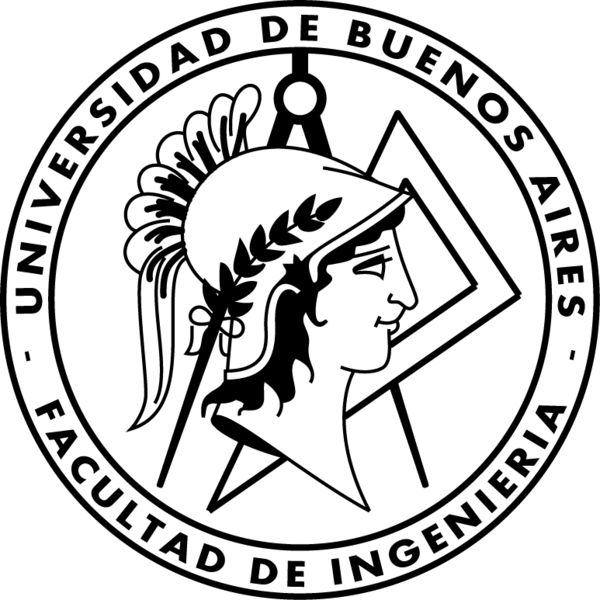
\includegraphics[width=7.5cm, height=7.5cm]{images/logo}
    \end{center}

    \materia{Organización de Datos}
    \submateria{Segundo Cuatrimestre 2017}
    \titulo{Trabajo Práctico 1}

    \integrante{Rodrigo De Rosa}{97799}{rodrigoderosa@outlook.com}
    \integrante{Marcos Schapira}{97934}{schapiramarcos@gmail.com}
    \integrante{Facundo Guerrero}{97981}{facundoiguerrero@gmail.com}
    \maketitle
    %Fin caratula
    %Table of contents
    \newpage
    \pagenumbering{roman}
    \tableofcontents
    %Fin table of contents
    %Informe
    \newpage
	\pagenumbering{arabic}
	\part{Análisis del precio por $m^2$}
		\section{Adaptación del DataFrame}
			Para el análisis particular de cada característica de la información que se posee, se adaptó el DataFrame
			original para poder analizar dicha información mas fácil y comodamente.
			\subsection{Filtrado de columnas}
				Para el análisis de esta cierta característica de las propiedades, consideramos \emph{importantes}
				sólo a algunas celdas. Estas son:
				\begin{itemize}
					\item \code{place name} $\leftarrow$ \code{location}
					\item \code{price aprox usd} $\leftarrow$ \code{price}
					\item \code{surface total in m2} $\leftarrow$ \code{totalSurface}
					\item \code{surface covered in m2} $\leftarrow$ \code{coveredSurface}
					\item \code{price usd per m2} $\leftarrow$ \code{pricem2}		
				\end{itemize}
			\subsection{Completando el DataFrame}
				Lo primero que se hizo para realizar este analisis fue completar las columnas faltantes
				de la mayor cantidad de entradas posibles. Esto es, \code{location, price, totalSurface,
				pricem2}. De esta forma, nos permitimos analizar una mayor cantidad de propiedades
				para realizar un analisis un poco mas correcto. \\
				\tab Para completar el campo de precio por $m^2$ se necesita que la entrada sobre la que
				se trabaja cumpla la siguiente condición lógica: $price_{}m^2 \vee (price \wedge surface)$. Es
				decir, necesita tener o el precio por metro cuadrado o tanto el precio total como la superficie
				total. \\
				\tab Si el campo \code{pricem2} tiene valor, entonces ese será el utilizado. En caso contrario,
				si tanto el campo \code{price} como el campo \code{totalSurface} tienen valor, definimos como
				nuestro nuevo \code{pricem2} a la división $\frac{price}{surface}$. \\
				\tab Para esto, necesitamos unificar \code{coveredSurface} y \code{totalSurface}, para maximizar
				nuevamente la cantidad de entradas disponibles. Esto se hace, simplemente, poniendo como
				\code{totalSurface} el valor de \code{coveredSurface} en aquellas entradas donde la primera
				no tenga valor (consideramos que $total - covered = uncovered$). \\
				\tab Una vez completados todos los \code{pricem2} posibles, eliminamos todas aquellas entradas
				que tengan \code{NaN} como valor (en cualquiera de las celdas que definimos como \emph{importantes}),
				pues ya no podemos obtener el valor de esa celda de ningun otro lugar.
		\section{Estudio estadístico de los datos}
			\subsection{Analisis de la distribución de precios}
				Una vez completado el DataFrame lo mas posible, se realizó un análisis de la distribución de precios.
				Con esto nos referimos a analizar la variación del precio por metro cuadrado entre todas las
				propiedades. Es decir, \emph{limpiar los datos que no tienen sentido}. \\
				\tab Para esto le pedimos el \code{.describe()} a nuesto DataFrame con los percentiles $0.01$ y
				$0.99$. Esto nos permite analizar que tan desviados estan los valores máximos y mínimos. \\
				\tab Con los percentiles recién mencionados hacemos un recorte de los datos para lograr una distribución
				que se asemeje a una Normal lo mas posible. El primer recorte es tanto inferior ($ > 150$USD) como superior
				($<18000$USD). Como en este nuevo DataFrame la diferencia entre el percentil $0.99$ y el máximo es de más
				del doble, se vuelve a recortar superiormente ($<8000$USD). \\
				\tab Luego de esto, la distribución de precios es un poco mejor que antes (las diferencias entre los
				percentiles $0.25, 0.5, 0.75$ son similares). \\
				\tab A continuación se muestra un gráfico de distribución de precios por metro cuadrado que se obtiene
				del DataFrame original sin realizar el filtrado recién mencionado. Nos hubiese gustado poder mostrar tanto
				el KDE como el histograma pero al haber tanta diferencia entre el maximo y los valores principales de la
				distribución, el histograma era solo una linea. El objetivo de este gráfico es hacer incapié en lo mencionado
				en el previo párrafo: es necesario filtrar los datos para tener un conjunto de datos con sentido.
				\begin{center}
       				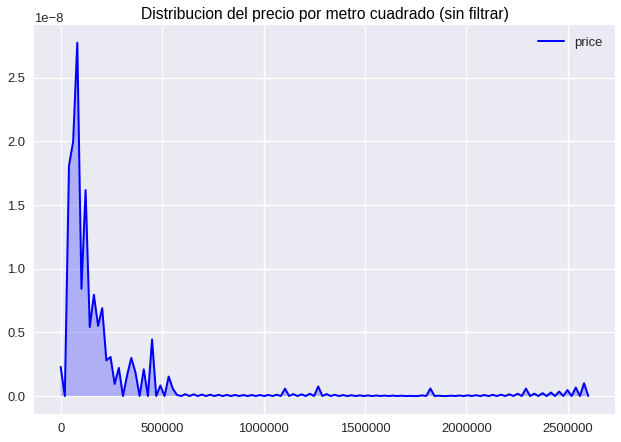
\includegraphics[width=\textwidth]{images/m2UnfilteredKDE}
		   		\end{center}
				\tab En el siguiente gráfico de distribución de precios por metro cuadrado se puede ver que la mayor parte
				de las propiedades están concentradas en el rango de precios $[150;4000]$USD y luego hay un drástico decaimiento
				de cantidad de propiedades para el resto de los precios. Si bien se podría considerar que un recorte sería
				correcto, a partir de fuentes externas se sabe que ciertos barrios (\emph{i.e.} Puerto Madero) tienen,
				aproximadamente, un valor medio de $6000$USD por metro cuadrado.
				\begin{center}
       				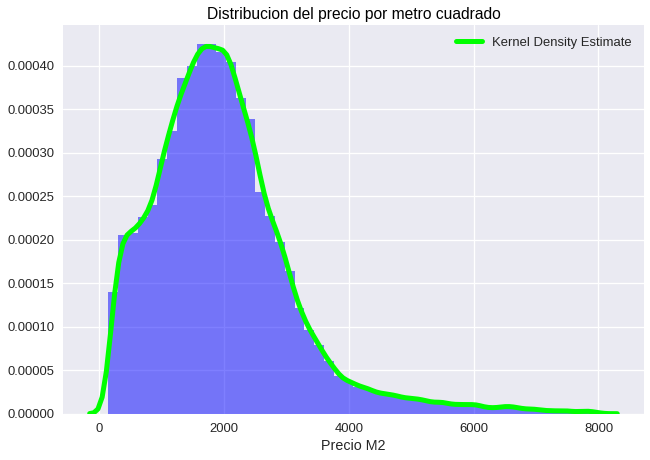
\includegraphics[width=\textwidth]{images/m2Histogram}
		   		\end{center}
			\subsection{Agrupando por barrios}
				Ahora que nuestros datos están tan completos y retocados como querríamos, procedemos a agrupar todas las propiedades
				de acuerdo al barrio al que pertencen. Una vez que los tenemos agrupados, debemos establecer un \emph{minimo de
				propiedades} por barrio. Pues un barrio que tiene una o dos propiedades podría alterar el estudio de la
				informacion. \\
				\tab Nuevamente, para esta tarea utilizizamos \code{.describe()} y resolvemos que utilizaremos como cota inferior
				$50$ propiedades (dos mas que el equivalente a una publicación por mes en los últimos cuatro años). \\
				\tab Aquí, al igual que hicimos antes, mostraremos la distribución antes y después del filtro aplicado. Si bien
				en escencia no son tan diferentes, podemos observar que desaparecen algunos barrios de la zona de precios altos.
				\begin{center}
       				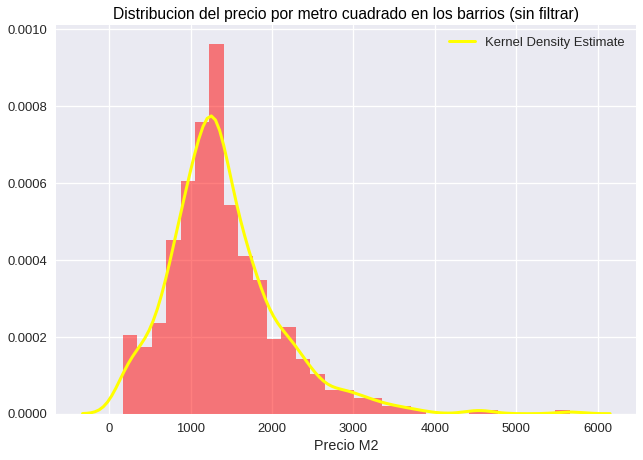
\includegraphics[width=\textwidth]{images/m2HoodUnfilteredKDE}
		   		\end{center}
				\tab Una vez que eliminamos los barrios problemáticos, si analizamos la distribución de precio por barrio
				podemos ver que la mayor parte está concentrada en el intervalo $[500;3500]$USD, mientras que muy pocos
				(solo tres) superan ese valor.
				\begin{center}
   	    				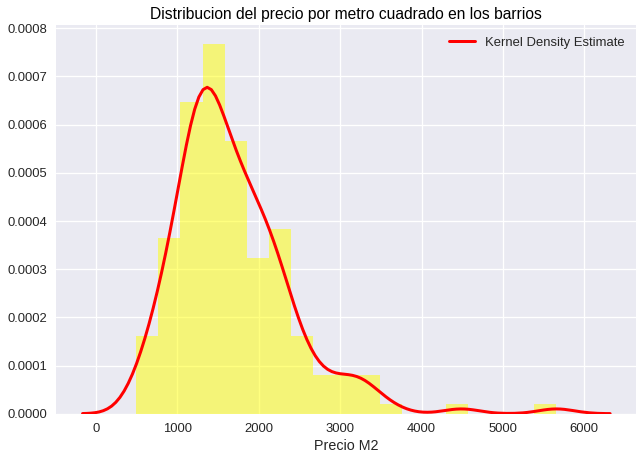
\includegraphics[width=\textwidth]{images/m2HoodHistogram}
			    \end{center}	
			    \tab Podemos ver, además, que la distribución es bastante similar a la anterior (sin agrupar por barrios) aunque,
			    obviamente, con valores menores (pues son promedios).
		\section{Analizando grupos característicos}
			En esta sección analizaremos ciertos grupos característicos a partir de la información con la que estamos trabajando.
			\subsection{Los diez barrios con mayor precio por $m^2$}
				Dado que ya estamos felices con la forma en que tenemos dispuestos los datos, comenzaremos por hacer un
				\emph{Top 10} de los barrios más caros de CABA y GBA. \\
				\tab Para esto, como ya tenemos los datos agrupados, simplemente ordenamos el DataFrame y nos quedamos con
				los primeros diez.
				\tab Durante el análisis de esta información, notamos que varios de los barrios que aparecían en este \emph{Top 10}
				eran subdivisiones del barrio de Palermo. Por esta razón, decidimos incluir dos casos: uno en que consideramos
				que todos los 'Palermos' son uno solo, y otro en que cada uno es considerado un barrio diferente.
				\subsubsection{Unificación de Palermo}
					En este caso, consideramos que todas las subdivisiones de Palermo pertenecen a un sólo barrio.\\
					\tab El resultado obtenido es el siguiente:
					\begin{center}
						\begin{tabular}{ |c|c|c| }
							\hline
							\multicolumn{3}{|c|}{Top 10 [Palermo unificado]}\\
							\hline
							\hline
							Puesto & Barrio & Precio $m^2$ [U$\$$D] \\
							\hline
							1 & Puerto Madero & 5657 \\
							2 & Las Cañitas & 3612 \\
							3 & Palermo & 3518 \\
							4 & Recoleta & 3316 \\
							5 & Belgrano & 3124 \\
							6 & Nuñez & 3056 \\
							7 & Barrio Norte & 2949 \\
							8 & Vicente López & 2925 \\
							9 & Retiro & 2783 \\
							10 & Olivos & 2737 \\
							\hline
						\end{tabular}
					\end{center}
					\tab En la tabla se observa que Puerto Madero tiene un valor mucho mas alto que el resto, de hecho, es
					mayor al doble del precio del décimo. De todos modos, entre el segundo y el último la variación es más
					suave. Para aportar a este análisis, se realiza un gráfico de barras:
					\begin{center}
   	    					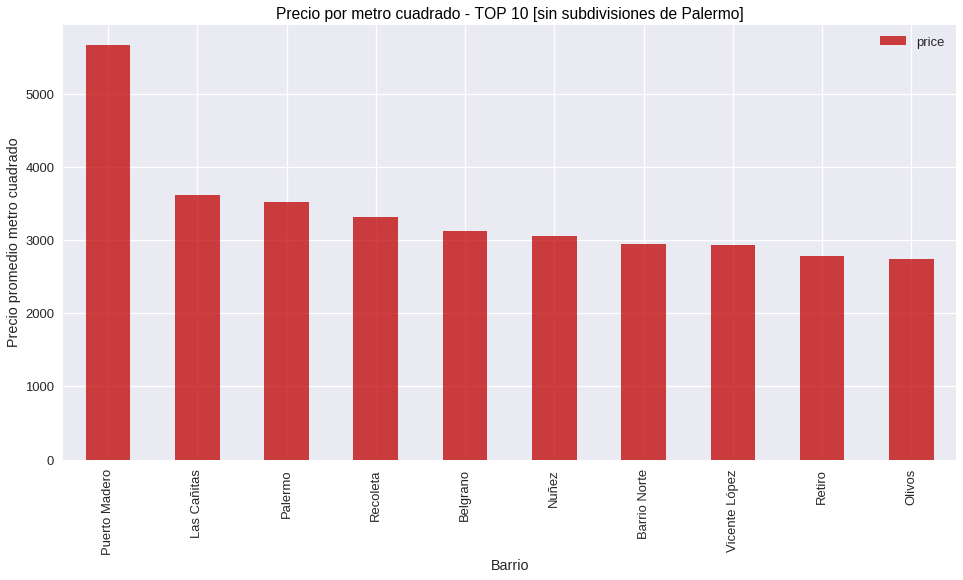
\includegraphics[width=\textwidth]{images/m2UnifiedTop10}
			  		\end{center}	
			  	\subsubsection{División de Palermo}
			  		Aquí consideraremos que el barrio al que se nombra Palermo corresponde a todas las secciones de dicho
			  		barrio que no son las que ya aparecen en otro grupo. \\
			  		\tab En este caso, el resultado obtenido es:
			  		\begin{center}
						\begin{tabular}{ |c|c|c| }
							\hline
							\multicolumn{3}{|c|}{Top 10 [Palermo dividido]}\\
							\hline
							\hline
							Puesto & Barrio & Precio $m^2$ [U$\$$D] \\
							\hline
							1 & Puerto Madero & 5657 \\
							2 & Palermo Chico & 4489 \\
							3 & Las Cañitas & 3612  \\
							4 & Palermo Viejo & 3419 \\
							5 & Recoleta & 3316 \\
							6 & Palermo & 3260 \\
							7 & Palermo Hollywood & 3224 \\
							8 & Palermo Soho & 3198 \\
							9 & Belgrano & 3124 \\
							10 & Nuñez & 3056 \\
							\hline
						\end{tabular}
					\end{center}
					\tab En la tabla podemos ver que, si bien es correcto y es un \emph{Top 10}, esta plagado de subdivisiones
					de Palermo y no nos permite tener un plano más general. \\
					\tab Aquí el gráfico de barras es muy similar aunque aparece Palermo Chico, que se acerca un poco mas
					al valor de Puerto Madero. De todos modos, la diferencia entre el primero y el segundo es muy grande
					como también lo es entre el segundo y el tercero, dejando la relación entre los valores igual de 'no suave'.
					\begin{center}
   	    					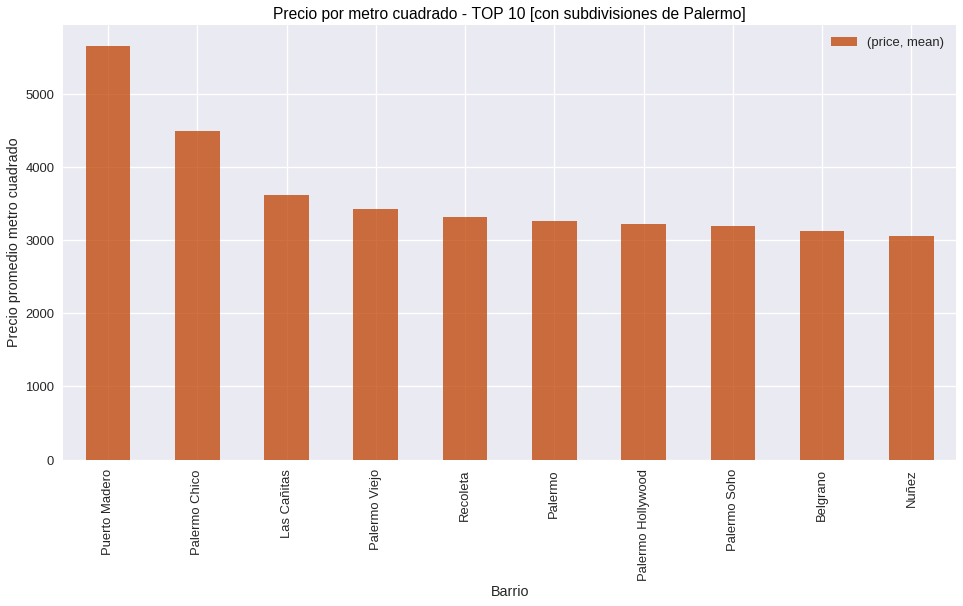
\includegraphics[width=\textwidth]{images/m2NotUnifiedTop10}
			  		\end{center}
			  		\tab De aquí en más, utilizaremos a Palermo como un barrio unificado.
			  	\subsubsection{Comentario sobre el Top 10}
				  	Este \emph{Top 10} arroja los resultados que se hubieran esperado, pues los únicos dos valores que no pertenecen
			  	a CABA corresponden a los primeros dos barrios de GBA en los que se piensa al pensar en los barrios mas caros
			  	de Buenos Aires. \\
			  		\tab Por otro lado, si nos sorprende el hecho de que el $m^2$ en Barrio Norte sea más barato que Núñez o en
			  		Belgrano.
			\subsection{Los diez barrios con menor precio por $m^2$}
				Para esta parte, al igual que antes, ordenamos los datos para analizar cuales son los diez barrios que se encuentran
				en el \emph{Bottom 10}. \\
				\tab Al realizar este análisis, lo obtenido es:
				\begin{center}
					\begin{tabular}{ |c|c|c| }
						\hline
						\multicolumn{3}{|c|}{Bottom 10}\\
						\hline
						\hline
						Puesto & Barrio & Precio $m^2$ [U$\$$D] \\
						\hline
						1 & Ingeniero Pablo Nogués & 494 \\
						2 & Maschwitz & 548 \\
						3 & Villa Udaondo & 558 \\
						4 & Parque Leloir & 579 \\
						5 & Presidente Perón & 643 \\
						6 & Benavidez & 705 \\
						7 & José C Paz & 711 \\
						8 & Villa Libertad & 743 \\
						9 & Longchamps & 800 \\
						10 & Burzaco & 804 \\
						\hline
					\end{tabular}
				\end{center}
				\tab Si graficamos estos valores al igual que antes podremos ver un ascenso (o descenso) más suave que el del
				\emph{Top 10}. Si bien el primero es casi la mitad de el último, la variación entre puestos es menor. \\
				\begin{center}
   	    				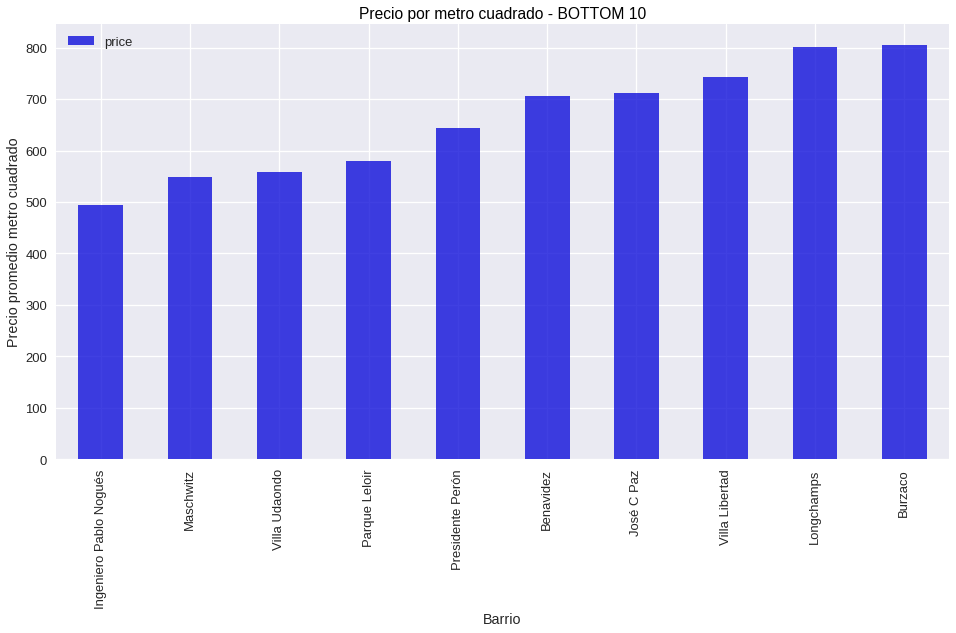
\includegraphics[width=\textwidth]{images/m2Bottom10}
			  	\end{center}
				\tab Aquí, remitiéndonos a la sección 3.1.3, vemos que los barrios del \emph{Bottom 10} son todos barrios
				alejados de la ciudad, de los cuales es esperable un bajo valor del $m^2$.
			\subsection{Dividiendo en secciones}
				El objetivo de esta parte es determinar diferentes grupos de barrios basados en el precio promedio del $m^2$
				para, de esta manera, analizar que tan suave (o no) es el decrecimiento del valor del $m^2$ en cada uno de
				estos grupos. \\
				\tab Los barrios serán divididos en grupos a partir de valores arbitrarios de precio por $m^2$, que surgen de
				un análisis de los datos. Los grupos serán:
				\begin{center}
					\begin{tabular}{ |c|c|c| }
						\hline
						\multicolumn{3}{|c|}{Divisones} \\
						\hline
						\hline
						Numero & min(price$m^2$) [USD] & max(price$m^2$) [USD] \\
						\hline
						1 & $2500$ & $\infty$ \\
						\hline
						2 & $2000$ & $2499$ \\
						\hline
						3 & $1500$ & $1999$ \\	
						\hline
						4 & $1200$ & $1499$ \\
						\hline
						5 & $950$ & $1199$ \\		
						\hline
						6 & $450$ & $949$ \\			
						\hline
					\end{tabular}
				\end{center}
				\tab El siguiente gráfico de área muestra el precio del $m^2$ y las divisiones (diferentes intensidades de
				azul) indican los diferentes grupos.
				\begin{center}
   	    				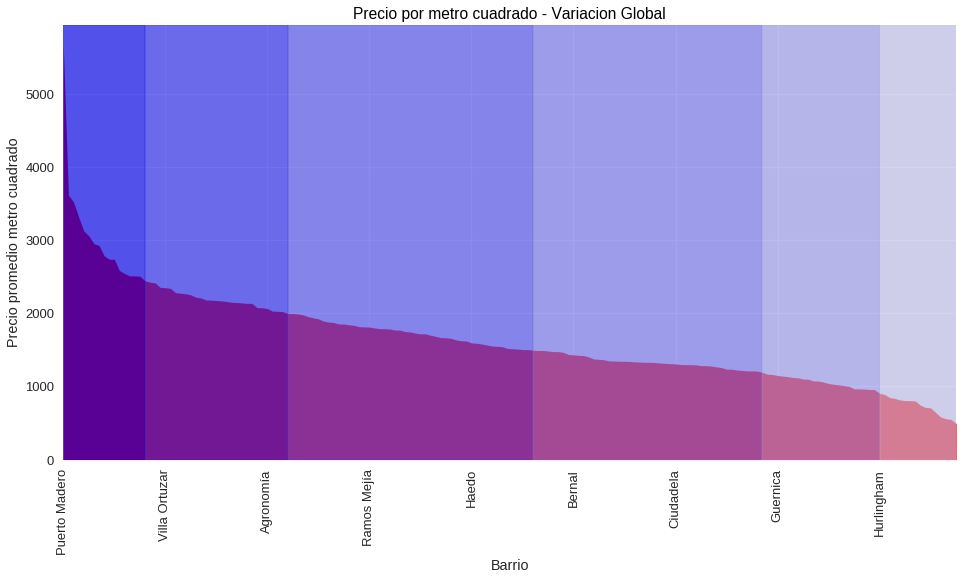
\includegraphics[width=\textwidth]{images/m2HoodsDivision}
			  	\end{center}
			  	\tab Nos interesa mostrar también que porcentaje de los barrios está incluído en cada uno de estos grupos para
			  	saber en cuál de ellos se concentra la mayor parte.
			  	\begin{center}
			  		\begin{tabular}{ |c|c|c| }
						\hline
						\multicolumn{3}{|c|}{Distribución en grupos} \\
						\hline
						\hline
						Grupo & Cantidad de barrios & Porcentaje \\
						\hline
						1 & 16 & $9\%$ \\
						\hline
						2 & 28 & $16\%$ \\
						\hline
						3 & 48 & $27\%$ \\
						\hline
						4 & 45 & $26\%$ \\
						\hline
						5 & 23 & $13\%$ \\
						\hline						
						6 & 16 & $9\%$ \\
						\hline						
			  		\end{tabular}
				\end{center}			  	 
				\tab Vemos que, como se puede apreciar en el gráfico, los grupos $3$ y $4$ son los que concentran a la mayor
				cantidad de barrios. De hecho, entre ellos dos tienen a más del $50\%$. \\
				\tab Ahora procedermos a analizar grupo por grupo.
				\subsubsection{Grupo 1 - $[2500:\infty)$U$\$$D}
					En este grupo se encuentra a los dieciséis barrios más caros de CABA y GBA. Aunque a los primeros diez ya los
					conocemos de la sección 3.1, lo que nos interesa en esta parte es analizar y comparar cómo varía el precio
					del metro cuadrado grupo a grupo mas que los nombres propios de cada integrante de cada grupo. En cada uno
					de los grupos se mostrará un \emph{zoom} del gráfico de área previo, para agregar una visualización al
					análisis de la variación en cada caso. \\
					\tab En este caso, lo que esperamos encontrar es un inicio con una pendiente muy inclinada y, a medida que
					nos alejamos del primer barrio (que ya sabemos que es Puerto Madero), un decrecimiento de dicha pendiente,
					pues la diferencia entre barrio y barrio será mucho menor, aunque seguirá siendo el grupo con mayor variación
					entre barrios de todos.
					\begin{center}
   		    				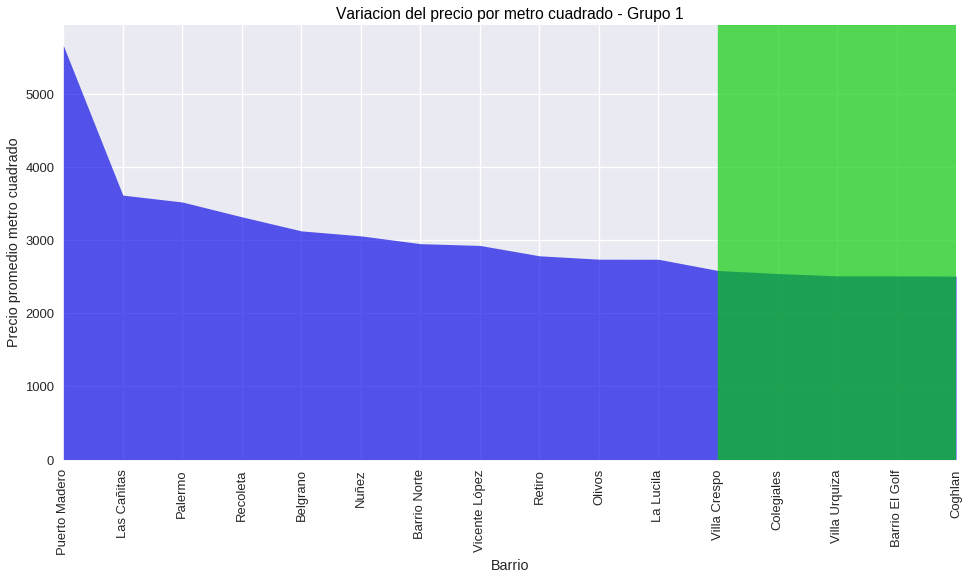
\includegraphics[width=\textwidth]{images/m2Group1Area}
				  	\end{center}
				  	\tab Si bien el gráfico muestra lo que se esperaba, también se ve que a partir del doceavo barrio la curva
				  	se vuelve casi constante (en verde), mostrando que hay un cierto subgrupo de barrios con precios muy 
				  	similares. Esto se puede ver en el gráfico de la sección anterior si se observa el pequeño valle que 
				  	se forma justo antes 	de llegar a la división entre el grupo 1 y el 2. \\
				  	\tab Cabe destacar, además, que si no fuera por el precio extraordinario de Puerto Madero, el grupo tendría
				  	una variación mucho menor, pues iría entre $3600$USD y $2500$USD lo que representaría una variación de
				  	$1100$USD ($30\%$) entre el máximo y el mínimo mientras que, actualmente, la variación es de $3100$USD
				  	($55\%$).
				\subsubsection{Grupo 2 - $[2000:2500)$U$\$$D}
					Observando el gráfico en el que se realizaron las divisiones por grupo esperamos que este segundo grupo
					tenga un sector medio con pendiente casi nula, donde la diferencia entre el precio en un barrio y el
					siguiente sea casi nula.
					\begin{center}
   		    				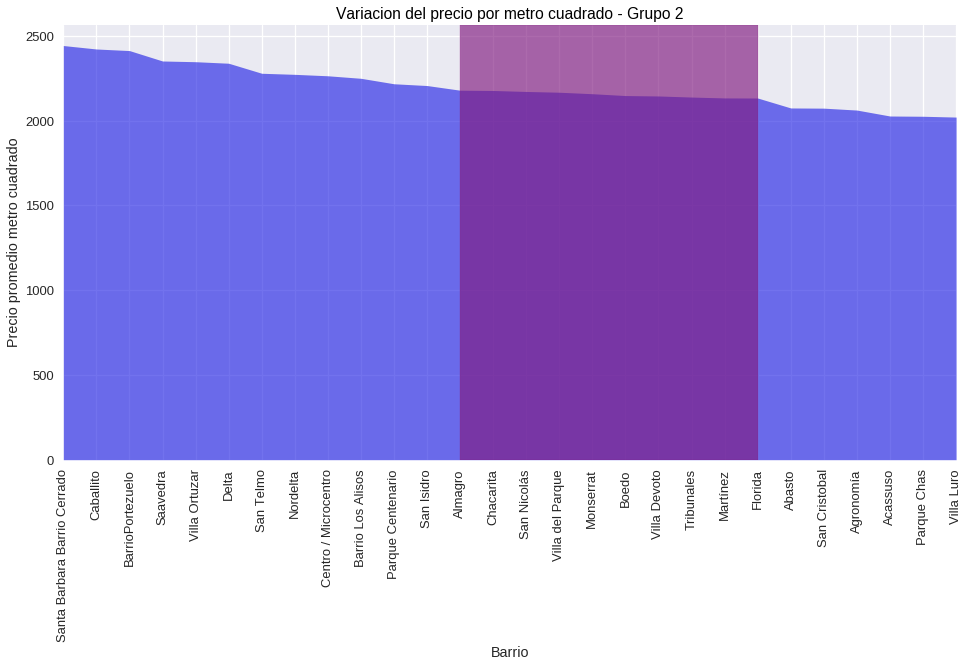
\includegraphics[width=\textwidth]{images/m2Group2Area}
				  	\end{center}
				  	\tab El sector indicado el violeta es aquel que mencionamos previamente con pendiente casi nula. En este
				  	subgrupo se encuentran diez barrios y la diferencia entre el primero y el último es de solamente $46$USD.
				  	Dado los numeros que se manejan, esa diferencia es casi despreciable, teniendo así un subgrupo de diez 
				  	barrios con el mismo valor para el $m^2$. \\
				  	\tab En cuanto al porcentaje de variación, a partir de este segundo grupo lo podemos dividir en dos; uno
				  	particular del grupo, en donde el porcentaje se calcula a partir del máximo local, y otro general, en donde
				  	el porcentaje se calcula a partir del máximo global (\emph{i.e.} Puerto Madero). La diferencia entre el
				  	máximo local y el mínimo es de $422$USD, siendo, de esta manera, la variación local del $17\%$ y la general
				  	del $7\%$. \\
				  	\tab Vemos entonces que la diferencia de variación ya decreció en gran medida pasando del grupo 1 al grupo 2.
				\subsubsection{Grupo 3 - $[1500:2000)$U$\$$D}
					Ahora llegamos al primero de los dos grupos principales. Como vimos antes, este grupo concentra al $27\%$ de
					los barrios de CABA y GBA pero (según nos muestra a grandes rasgos el gráfico general) con mayor variación
					que el próximo grupo, que también concentra a una gran parte de los barrios.\\
					\tab En este caso, esperamos ver una pendiente casi constante en todo el grupo sin regiones con pendiente
					casi nula pero con una variación pequeña entre un barrio y el siguiente.
					\begin{center}
   		    				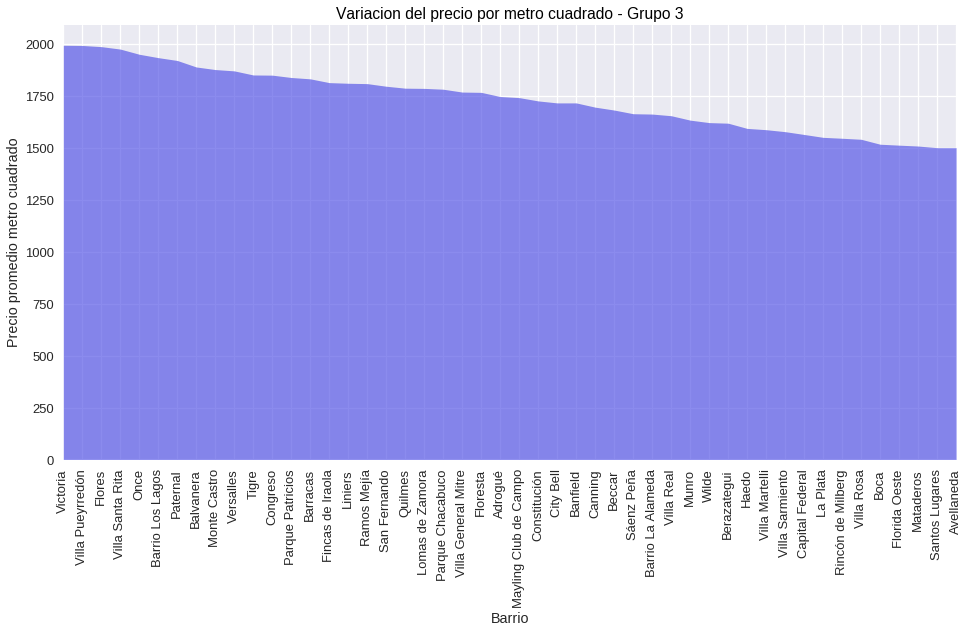
\includegraphics[width=\textwidth]{images/m2Group3Area}
				  	\end{center}
				  	\tab En este gráfico se observa lo previamente indicado, el decrecimiento es bastante lineal y no se detectan
				  	zonas con precios constantes. De todas formas, si se amplía un poco, se pueden encontrar pares o tríos de grupos
				  	que tienen precios similares, como se ve a continuación.
				  	\begin{center}
   		    				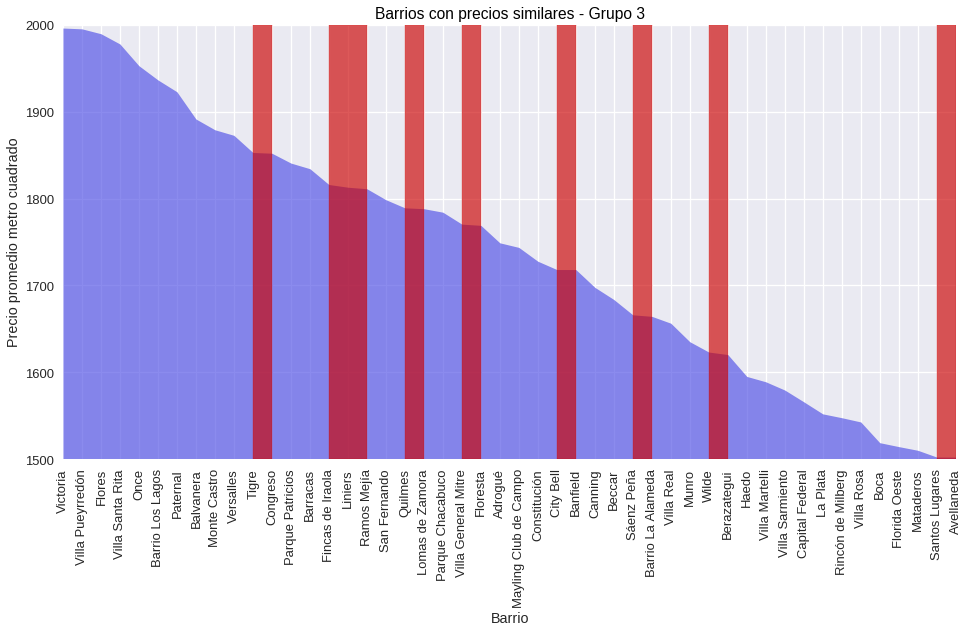
\includegraphics[width=\textwidth]{images/m2Group3Detail}
				  	\end{center}
				  	\tab Aquí podemos ver que si bien hay diecisiete barrios que comparten precio con algún otro, no son contiguos
				  	como en el grupo 2. De todas maneras, como en este grupo la variación general de precio es menor y la cantidad
				  	de barrios es mayor, podríamos encontrar también un grupo de diez barrios con variación de aproximadamente
				  	$50$USD. Por ejemplo, entre Monte Castro y Ramos Mejía hay una diferencia de $60$USD y se encierra un subgrupo
				  	de nueve barrios. \\
				  	\tab Analizando el porcentaje de variación al igual que en el Grupo 2, sabiendo que la diferencia entre el
				  	máximo local y el mínimo es de $493$USD, el porcentaje de variación local es de un $25\%$ y el porcentaje
				  	de variación global es del $9\%$. \\
				  	\tab Se observa entonces que, lógicamente, ahora que estamos en una zona de precios menores, una diferencia
				  	entre mínimo y máximo similar a la del grupo anterior ahora representa una variación mayor. Por otro lado,
				  	la variación global es apenas mayor a la del grupo anterior. De todas formas, estos porcentajes están sujetos
				  	a la división arbitraria de los grupos hecha previamente (pues el máximo delta es $500$USD).
				\subsubsection{Grupo 4 - $[1200:1500)$U$\$$D}
					Este cuarto grupo es el segundo grupo principal, concentra el $26\%$ de todos los barrios y es el de menor
					rango de valores, con $300$USD, salvo por el grupo 5, con $250$USD. Esto nos dice que la pendiente en este
					caso será la menor de todas, como se puede ver en el gráfico general. Además, esperamos ver una zona central
					con pendiente casi nula, en donde se encontrará un grupo muy grande de barrios con una variación en el precio
					muy pequeña, a diferencia del grupo 3.
					\begin{center}
   		    				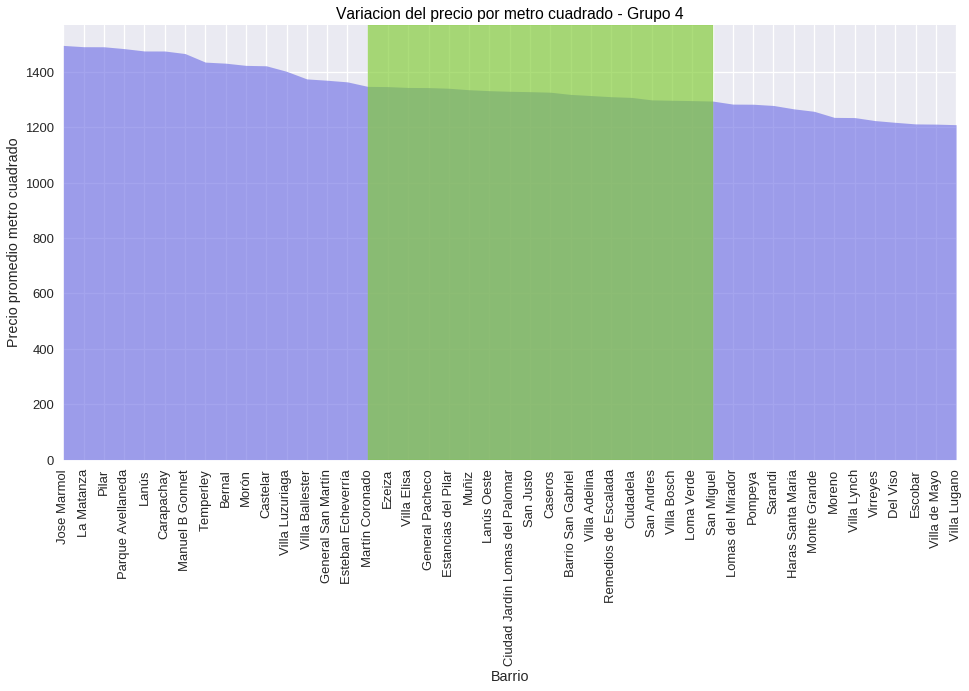
\includegraphics[width=\textwidth]{images/m2Group4Area}
				  	\end{center}
				  	\tab El subgrupo indicado con verde consiste de dieciocho barrios que se diferencian solamente, entre el primero
				  	y el último, por $53$USD. Como supusimos, en este grupo se encuentra el conjunto de barrios con variación casi
				  	nula más grande de todos. Adicionalmente, si se observa el gráfico con atención, en la mayor parte se encuentran
				  	subgrupos pequeños con valores casi constantes hasta que hay un pequeño descenso de precio, nuevamente un valor
				  	casi constante, etc. dividiendo el grupo en cinco o seis diferentes subgrupos pequeños (o no tanto, como el
				  	verde) por lo que no tiene sentido destacarlos como en el grupo 3, pues solo quedarían aquellos pequeños sectores
				  	donde la pendiente si toma valor considerable. \\
				  	\tab En cuanto al porcentaje de variación, sabiendo que la diferencia entre el máximo local y el mínimo es de
				  	$286$USD, tenemos un porcentaje de variación local del $19\%$ y uno global del $5\%$. Por lo tanto, y como era
				  	de esperarse, este grupo tiene los porcentajes mínimos en ambos casos; en el local porque tiene la mayor cantidad
				  	de segmentos casi constantes y en el global porque, además de la razón recién mencionada, por tener valores
				  	cada vez más bajos. Cabe destacar, además, que el $19\%$ local está concentrado en ciertos 'saltos' de un
				  	barrio a otro; pues, como mencionamos antes, la mayor parte del grupo esta compuesta por subgrupos de precios
				  	similares.
				\subsubsection{Grupo 5 - $[950:1200)$U$\$$D}
					Este quinto y penúltimo grupo comienza una pendiente que incrementa progresivamente hacia el último y sexto
					grupo. Aquí se concentra el $13\%$ de los barrios, la mitad que en el grupo anterior, y los precios de los
					barrios ya se acercan a los minimos que se pueden encontrar.\\
					\tab A partir de la información que brinda el gráfico general, esperamos encontrar una pequeña zona de pendiente
					casi nula hacia el final del grupo y una variación local relativamente chica.
					\begin{center}
   		    				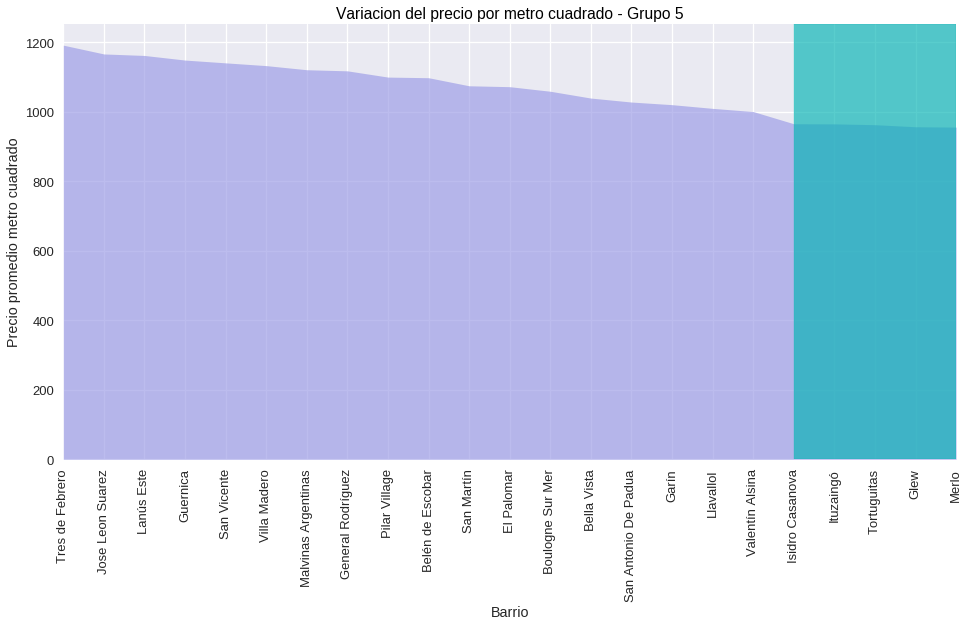
\includegraphics[width=\textwidth]{images/m2Group5Area}
				  	\end{center}
				  	\tab Indicado con color Cyan en el gráfico podemos ver ese pequeño grupo del que hablábamos donde la pendiente
				  	es casi nula, mientras que en el resto del grupo hay una pendiente casi constante. El tamaño de este subgrupo
				  	es de cinco barrios y la diferencia de precio entre el primero y el último es de $11$USD. \\
				  	\tab Si calculamos el porcentaje de variación, conociendo que la diferencia entre el máximo local y el mínimo
				  	es de $235$USD, obtenemos un porcentaje de variación local del $20\%$ y uno global del $4\%$. En este caso, el
				  	porcentaje local esta distribuido a lo largo de todo el grupo, salvo por el subgrupo final que tiene un valor
				  	casi constante.
				\subsubsection{Grupo 6 - $[450:950)$U$\$$D}
					En este último grupo, que contiene sólo al $9\%$ de los barrios (al igual que el grupo 1), estaremos analizando
					a aquellos barrios con menor precio por $m^2$. A partir del gráfico general sabemos que la pendiente será muy
					marcada y que la diferencia entre un barrio y el siguiente será importante, salvo por una pequeña parte donde
					los precios se mantendrán casi constantes.
					\begin{center}
   		    				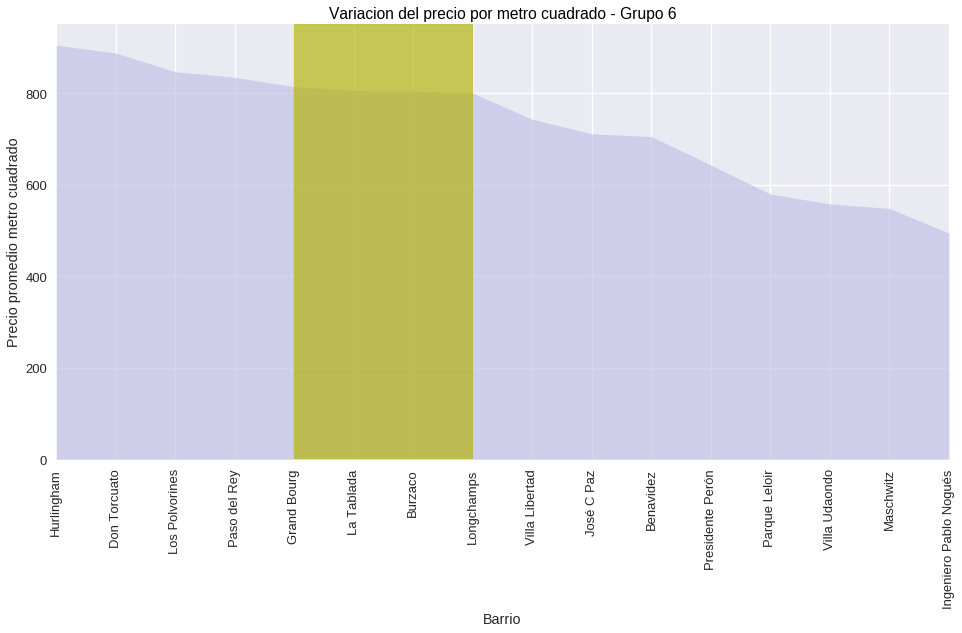
\includegraphics[width=\textwidth]{images/m2Group6Area}
				  	\end{center}
					\tab En amarillo se puede observar la única sección casi constante del grupo, que consta sólo de cuatro barrios
					y que contienen un rango cuya diferencia entre el mínimo y el máximo es de $14$USD. Mientras tanto, el resto
					del grupo tiene una pendiente considerablemente grande y la diferencia entre el valor máximo y el mínimo es casi
					del doble. \\
					\tab Para remarcar esto último, calcularemos el porcentaje de variación sabiendo que dicha diferencia es de
					$410$USD. El porcentaje de variación local es del $45\%$ y el porcentaje de variación global es del $7\%$. Aquí
					la variación local está repartida en todo el grupo pero con mayor participación de la segunda mitad, donde la
					pendiente es mayor, y con menor participación del sector casi constante.\\
		\section{Distribución geográfica}
			En esta sección se mostrará, con la ayuda de \emph{HeatMaps} cómo están distribuídos los precios por $m^2$ en CABA
			y GBA. \\
			\tab Para empezar, mostraremos un mapa general de CABA y GBA donde la unidad de medida es el precio por $m^2$. Se
			debe tener en cuenta que el software utilizado determina el color de un pixel a partir de la suma de todas las
			propiedades que se corresponden con ese pixel, y por dicha razón, podríamos encontrar sectores donde, si bien el
			precio no es tan elevado, hay muchas propiedades y por ende se las indica con rojo. De todas formas, este gráfico
			nos sirve para tener un plano general.
			\begin{center}
				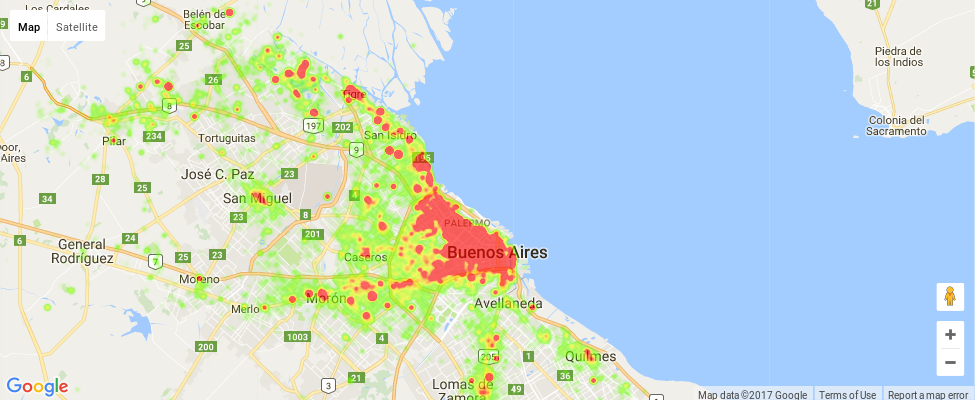
\includegraphics[width=\textwidth]{images/m2GeneralHeatMap}
		  	\end{center}
			\subsection{Grupos característicos y su ubicación}			
				Ahora, lo que haremos será repetir la dinámica pero dividiendo en los mismo grupos característicos de antes, para
				ver que se puede saber de cada grupo según su ubicación. Cabe destacar que la escala de precios utilizada en los
				mapas de cada grupo es diferente, pues el objetivo aquí es mostrar la ubicación de estos barrios más que el valor
				que ellos tienen.
				\subsubsection{Grupo 1}
					Para el grupo 1, como se dijo previamente, se espera encontrar a las propiedades en CABA y la zona de GBA
					que corresponde al inmediato Norte de la Capital Federal.
					\begin{center}
						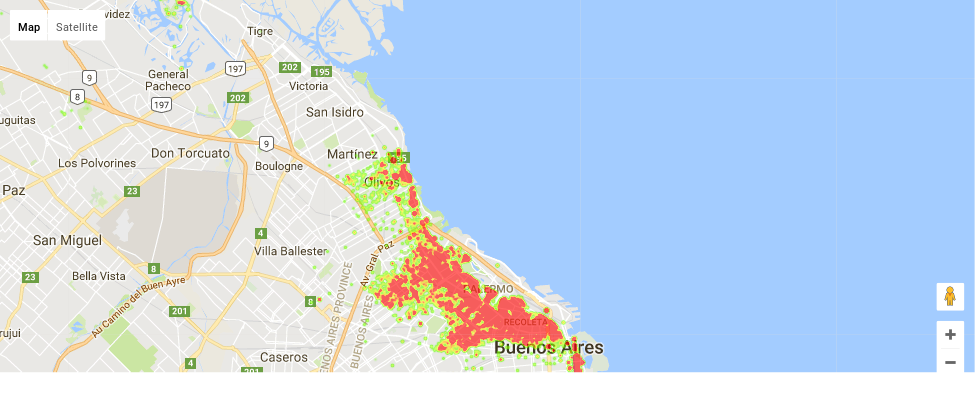
\includegraphics[width=\textwidth]{images/m2Group1HeatMap}
				  	\end{center}
				  	\tab En el gráfico se observa, más específicamente, que las propiedades con valores altos están ubicadas
				  	en el Este de la ciudad, esparciéndose desde el Microcentro hacia el Norte de CABA. Se puede ver, también,
				  	que las propiedades de la Provincia que se encuentran en este grupo son aquellas cercanas al río. Cabe destacar
				  	que Puerto Madero genera una 'discontinuidad' en el mapa, pues si se observa atentamente se ve que no está en
				  	una zona contigua al resto de los barrios. De todos modos, esto era de esperarse porque es un barrio construído
				  	específicamente como un 'lugar caro'. \\
				  	\tab Se debe mencionar, además, que el Barrio El Golf está ubicado en la localidad de Tigre y en este mapa no
				  	se lo puede ver. Se decidió dejarlo afuera para poder dar una mejor vista de la Capital Federal.
				\subsubsection{Grupo 2}
					Este segundo grupo se espera que esté compuesto por los barrios de capital y Zona Norte que no estaban presentes
					en el grupo previo. Esto es, San Isidro, Caballito, Saavedra, etc.
					\begin{center}
						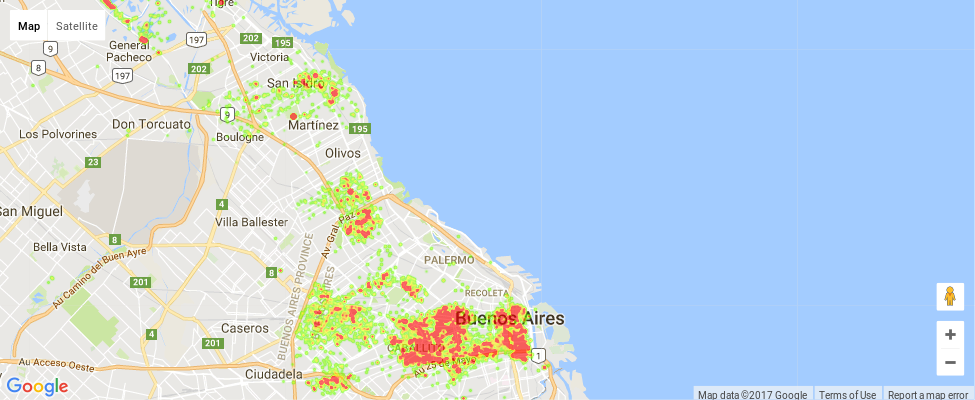
\includegraphics[width=\textwidth]{images/m2Group2HeatMap}
				  	\end{center}
				  	\tab El gráfico nos muestra que este segundo grupo contiene a los barrios del Sur Este de la Capital Federal
				  	('del centro para abajo', al revés que el grupo 1) y aquellos barrios que 'completan' la Zona Norte. Además, se
				  	encuentran algunos otros barrios dispersos, como por ejemplo Boedo. \\
				  	\tab Cabe destacar aquí también que en este segundo grupo se encuentran más barrios cerrados de la localidad de
				  	Tigre, como el Barrio Santa Bárbara y el Barrio Los Alisos, que nuevamente no se incluyeron en el mapa para
				  	poder dar más detalle a CABA.
				\subsubsection{Grupo 3}
					En este tercer grupo se espera que, además de que se cubra la mayor cantidad de superficie, se 'complete' la
					capital y comiencen a aparecer los barrios del llamado primer cordón del conurbano.
					\begin{center}
						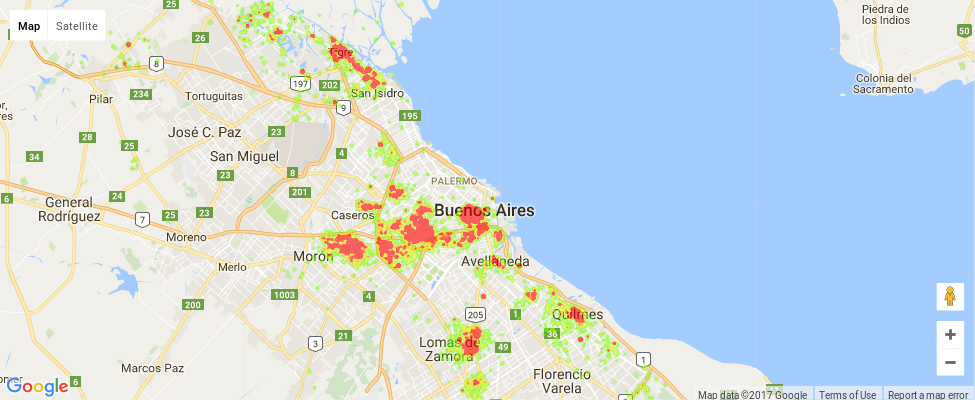
\includegraphics[width=\textwidth]{images/m2Group3HeatMap}
				  	\end{center}
				  	\tab El mapa presentado nos muestra, efectivamente, que está compuesto de los barrios restantes de la Capital
				  	Federal, algunos barrios del primer cordón, como Villa Martelli, Munro, Morón y otros más lejanos como Quilmes y
				  	Lomas de Zamora. Además, como se puede observar al Norte, se sigue completando la zona de barrios cerrados de la
				  	localidad de Tigre y sus alrededores. \\
				  	\tab También forma parte de este grupo la ciudad de La Plata pero se decidió dejarlo afuera de la visualización
				  	para poder enfocarnos más en CABA y GBA.
				\subsubsection{Grupo 4}
					Para este cuarto grupo, el segundo grupo principal como fue llamado previamente, se espera que se 'complete' el
					primer cordón del conurbano y comiencen a aparecer barrios del segundo y tercer cordón. También se espera que ya
					no aparezcan barrios de CABA.
					\begin{center}
						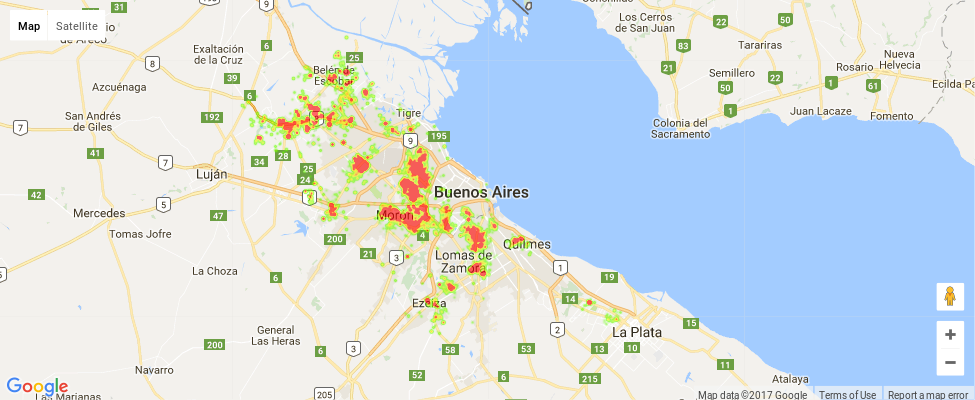
\includegraphics[width=\textwidth]{images/m2Group4HeatMap}
				  	\end{center}
				  	\tab En este caso se debió utilizar un nivel de zoom menor por la distancia entre los barrios del grupo. De todas
				  	maneras, se puede apreciar la aparición de más barrios del primer cordón del conurbano y de Pilar y Escobar, que
				  	son, al igual que Tigre, dos centros importantes de barrios cerrados y country clubs.
				\subsubsection{Grupo 5}
					Ya acercándonos a los barrios más baratos esperamos, tanto en este grupo como en el siguiente, encontrar
					barrios alejados de la Capital Federal pertenecientes al segundo y tercer cordón del conurbano.
					\begin{center}
						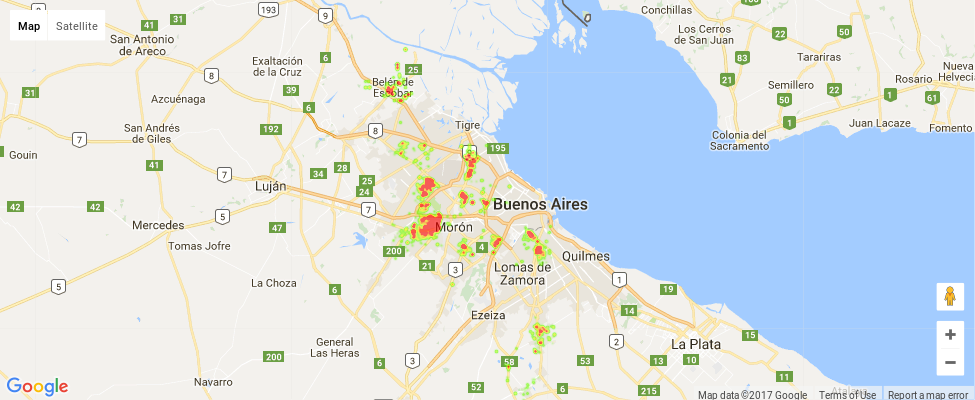
\includegraphics[width=\textwidth]{images/m2Group5HeatMap}
				  	\end{center}
				  	\tab Se puede observar que se completan algunas zonas faltantes del primer cordón del conurbano y aparecen zonas
				  	densas del segundo y tercer cordón, como se esperaba. De todas formas, al poseer cada vez menor cantidad de
				  	barrios, es más dificil hacer un mapa claro.
				\subsubsection{Grupo 6}
					Finalmente, en este sexto grupo esperamos encontrar barrios dispersos y alejados de la Capital Federal, con poca
					cantidad de propiedades.
					\begin{center}
						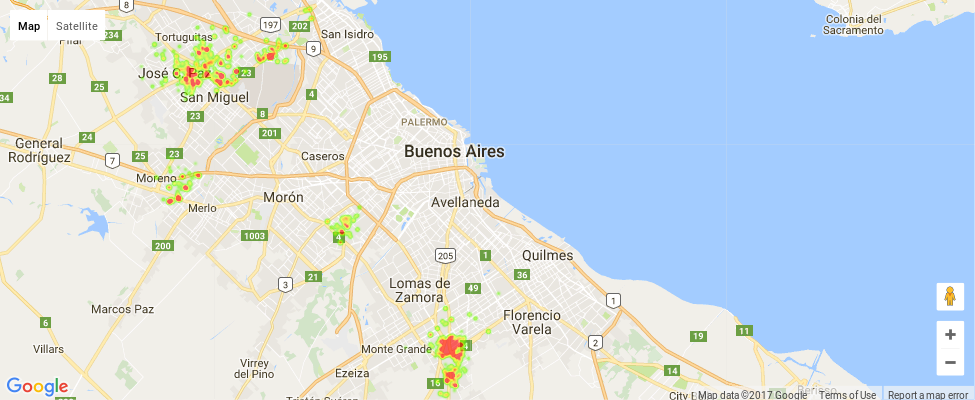
\includegraphics[width=\textwidth]{images/m2Group6HeatMap}
				  	\end{center}
				  	\tab Se verifica con este gráfico, entonces, que los integrantes de este último grupo pertencen al tercer,
				  	y más alejado, cordón del conurbano bonaerense.
				\subsubsection{Comparación de grupos}
					En este último gráfico mostraremos cómo se distribuyen los grupos en CABA y GBA, unificando todos los gráficos
					previos para un mejor entendimiento. Se utilizaron diferentes colores para diferenciar los grupos y dichos
					colores están indicados en la leyenda del gráfico.
					\begin{center}
						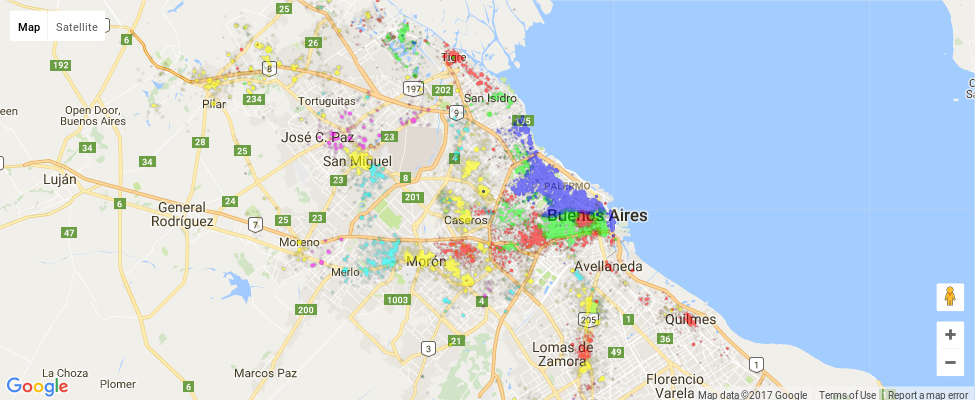
\includegraphics[width=\textwidth]{images/m2GroupComparison}
				  	\end{center}
		\section{Progresión del precio por $m^2$ a través de los años}
			En esta sección se analizará como fue progresando el valor del $m^2$ entre los años 2013 y 2017. Para esto,
			se realizaron gráficos particulares para cada año como así también dos gráficos que comparan a todos los años entre sí.
			\subsection{Fluctuación del precio del $m2$ a través de los años}
				Para comenzar, se mostrará un gráfico en el que se muestra la variación del precio del $m^2$ entre el año 2013 y el 
				año 2017.
				\begin{center}
					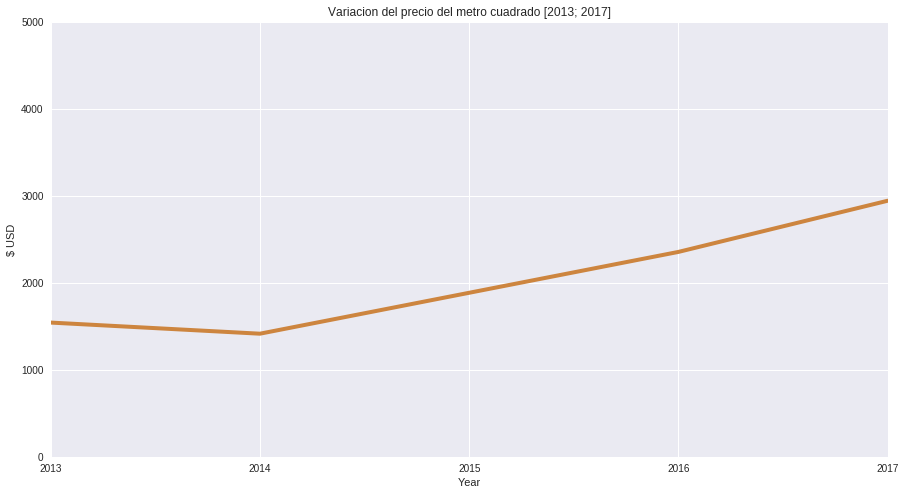
\includegraphics[width=\textwidth]{images/m2ProgressionGeneral}
				\end{center}
				\tab Se observa que entre 2013 y 2014 hubo un descenso del precio promedio pero que a partir de dicho año, el precio
				de las propiedades estuvo en aumento constante.
			\subsection{Año 2013}
				En este caso, se debe tener en cuenta que la cantidad de propiedad es la menor de todas y por lo tanto es posible
				que los precios disponibles no sean lo suficientemente representativos. De todas maneras, consideramos que es útil
				para un análisis comparativo con los años más recientes.
				\begin{center}
					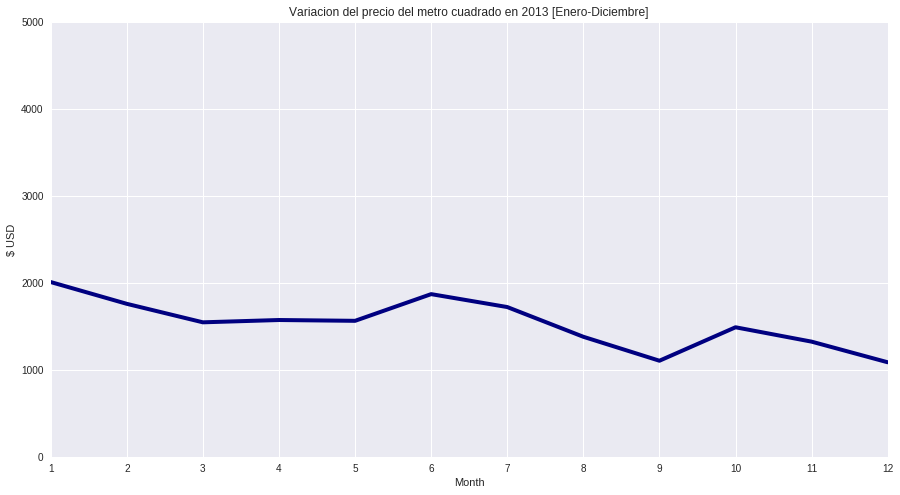
\includegraphics[width=\textwidth]{images/m2Progression2013}
				\end{center}
				\tab Se puede observar que el año 2013 tuvo una tendencia decreciente con aumentos sólo en los meses de Mayo
				y Septiembre.
			\subsection{Año 2014}
				Aquí la cantidad de propiedades ya es mayor, aunque muy menor a la de los años 2016 y 2017, de todas maneras, al
				igual que en el año anterior, es lo suficientemente descriptiva como para realizar una comparación más adelante.
				\begin{center}
					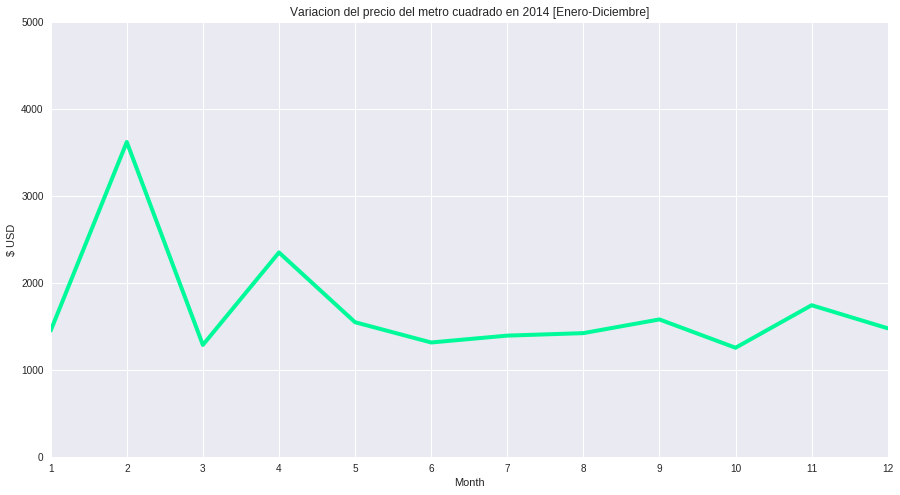
\includegraphics[width=\textwidth]{images/m2Progression2014}
				\end{center}
				\tab En este caso, vemos que hay una gran fluctuación de precios en los meses iniciales y finales pero se
				encuentra una región casi constante en los meses entre Mayo y Septiembre.  Podemos ver que, al igual que en 2013,
				el año termina con una baja del valor de $m^2$.
			\subsection{Año 2015}
				\begin{center}
					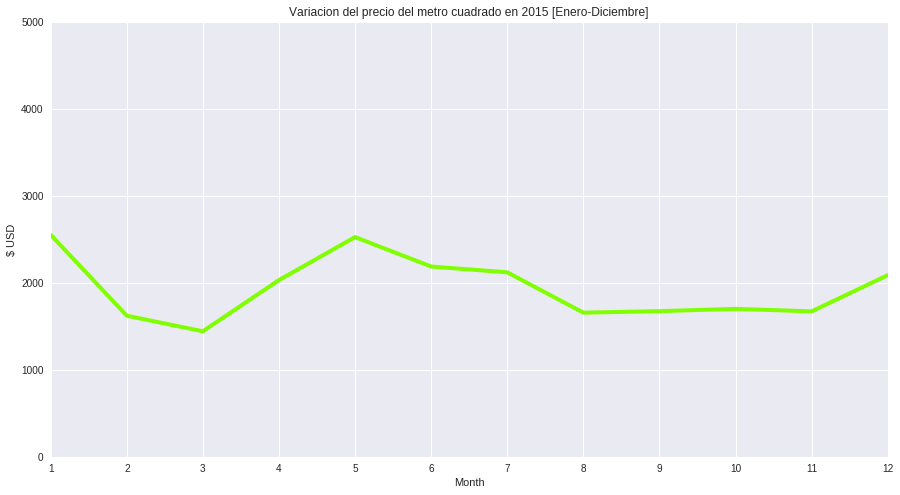
\includegraphics[width=\textwidth]{images/m2Progression2015}
				\end{center}
				\tab Podemos ver que este año comenzó con un decrecimiento del precio, luego volvió al precio de Enero y, luego de
				tres meses de precio constante, finalizó creciendo en Diciembre. Cabe destacar que el valor es bastante uniforme para
				los tres años hasta aquí analizados, aunque con un leve aumento.
			\subsection{Año 2016}
				\begin{center}
					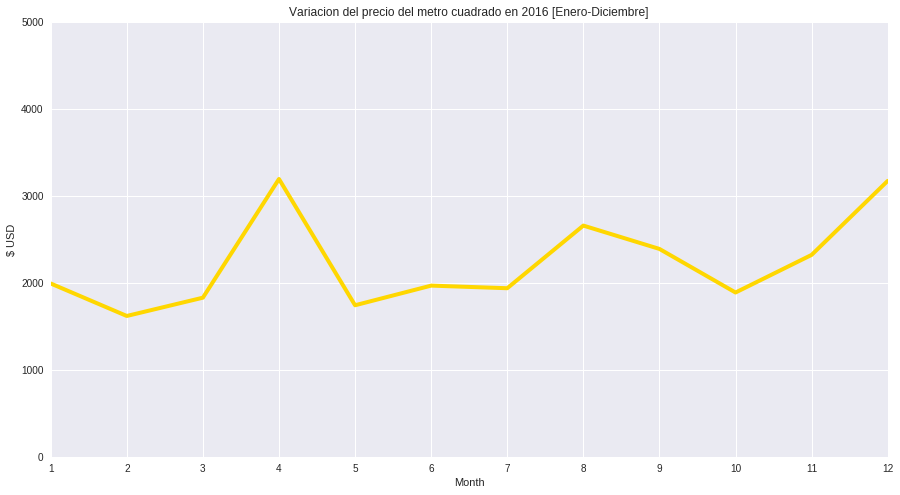
\includegraphics[width=\textwidth]{images/m2Progression2016}
				\end{center}
				\tab Este es, hasta aquí, el año con mayor fluctuación de precios. Con los decensos y ascensos más abruptos y con
				los valores más elevados. Se puede observar que el año finaliza con un aumento de precios muy importante, alcanzando
				el valor más alto hasta el momento.
			\subsection{Año 2017}
				Este es el año del que más información se posee, pues la información disponible es sobre publicaciones activas en
				la página oficial de \emph{Properati}. Obviamente, la información sólo llega hasta el mes de Agosto.
				\begin{center}
					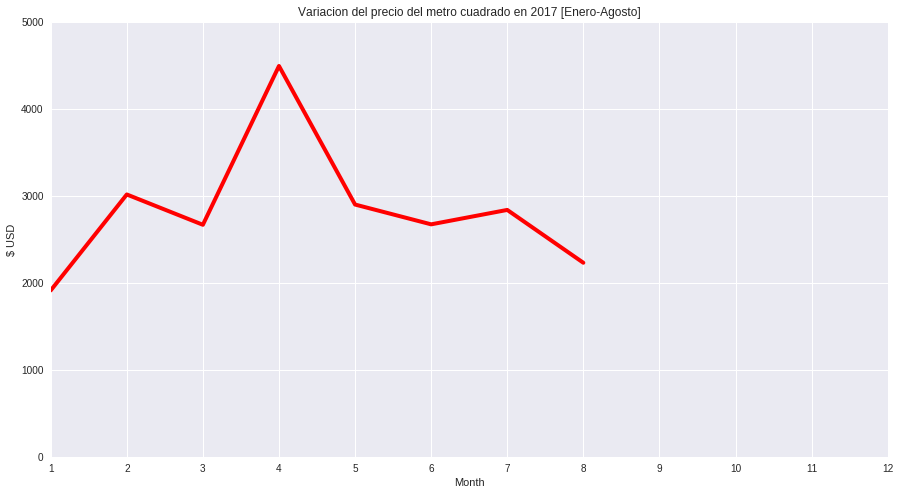
\includegraphics[width=\textwidth]{images/m2Progression2017}
				\end{center}
				\tab Aquí podemos ver que el año comenzó con un gran aumento, llegando a un pico de precios de los últimos cuatro
				años pero que, a partir del mes de Abril, comenzó el descenso y, para el mes de Agosto, ya casi se volvió a los
				valores de Enero.
			\subsection{Comparación de la progresión mensual en cada año}
				Ahora veremos dos gráficos en los que se unifica todo lo mostrado previamente, el cual nos permite comparar, año a
				año, cómo fue la variación de los precios. El primero es exactamente la superposición de los cuatro gráficos
				previos, mientras que el segundo (de barras) se utilizó para analizar mejor, mes por mes, en que año fue mayor
				el valor del $m^2$.
				\tab Comenzaremos analizando el mencionado gráfico de lineas:
				\begin{center}
					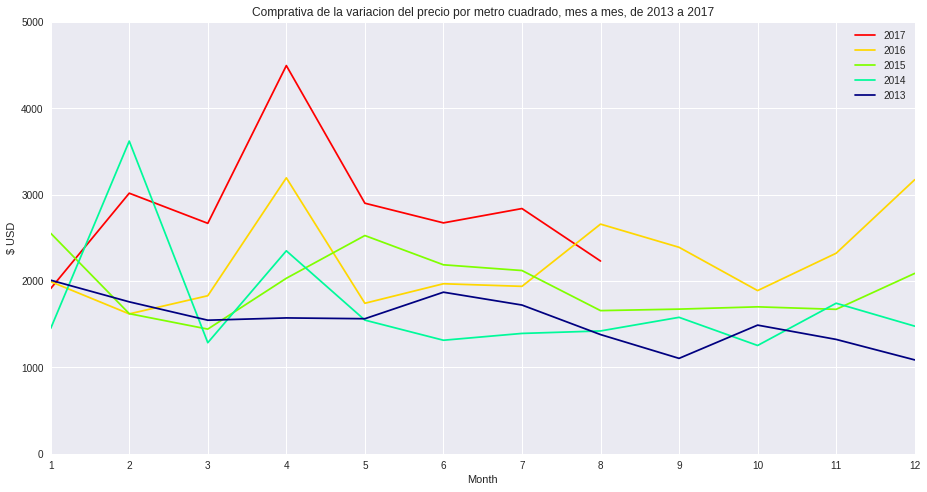
\includegraphics[width=\textwidth]{images/m2ProgressionLineComparison}
				\end{center}
				\tab Aquí podemos ver que el año 2017 (o al menos en lo que va del año) es el que mayores precios tiene en cinco de 
				los ocho meses en los que se posee información. Por otro lado, podemos ver que 2015 y 2016 terminan en suba mientras
				que 2013 y 2014 terminan en baja. También se puede ver que en los meses de Abril, Mayo y Junio hay una tendencia a
				suba de precios, mientras que no se encuentra una zona particular en la que haya tendencia a la baja de precios. \\
				\tab Ahora analizaremos el segundo gráfico, el de barras. El objetivo de este gráfico es, como se mencionó
				previamente, analizar, mes a mes, qué año tuvo los valores más altos.
				\begin{center}
					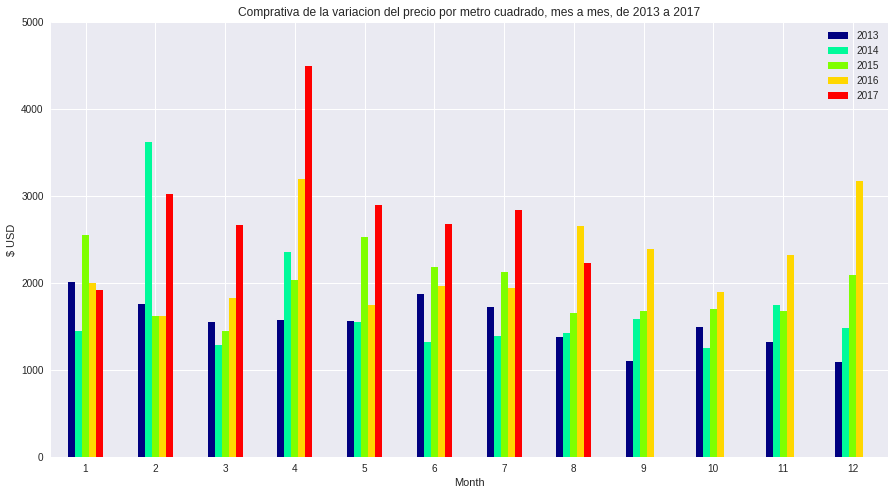
\includegraphics[width=\textwidth]{images/m2ProgressionBarComparison}
				\end{center}
				\tab Este gráfico permite ver que, si bien en 2017 se obtuvieron casi todos los valores récord en cada mes, mes a mes
				varía el orden de los años en cuanto a precio. Esto nos dice que los precios fluctuaron mucho en los últimos años
				aunque con una tendencia positiva (como ya vimos previamente), pues la mayoría de los máximos pertencen a años
				recientes.
		\section{Análisis de precio aproximado.}
	      	\subsection{Objetivo}
    				Esta sección tiene el objetivo de analizar como fueron variando los precios de las distintas propiedades en los
    				últimos 4 años. Con fin introductorio, se quiere brindar una mirada global acerca de la fluctuación de los precios
    				de todas las propiedades a lo largo de los últimos 4 años.
	      \subsection{Preparación y procesamiento de los datos}
			Para procesamiento de los datos, primero se separaron y agruparon los features por años. A continuación, para cada
			dataframe formado, es decir para las propiedades de un determinado año, lo que se hizo fue separarlas por meses. Entonces
			hasta el momento tenemos las propiedades separadas por años y por meses. Por último para cada año, se agruparon todas las
			propiedades de un mismo mes dejando como valor el precio en dolares promedio de las mismas. \\
       		\tab Por último, algo importante a tener en cuenta es que el set de datos esta referido a publicaciones y no a ventas de
       		propiedades en sí. Dichas publicaciones dejan de existir una vez que la propiedad fue vendida, por lo que los datos del
       		2013-2014 tal vez no sean lo suficientemente representativos por la cantidad de entradas que poseen, como si lo son los
       		datos del 2015 en adelante. De todas maneras, se usaron con fines representativos en el siguiente análisis. 

	      \subsection{Presentación de los gráficos de promedios}
	      	Aquí se muestran los gráficos que representan los promedios anteriormente mencionados para cada año. Vale aclarar que en
	      	los siguientes 5 gráficos el eje x representa los meses de cada año, y el eje y representa el precio de las propiedades
	      	en USD. Dicho precio varia entre 0$-$450000 $usd$, para obtener una mirada objetiva de los gráficos que serán presentados
	      	acontinuación.
			\begin{center}
       			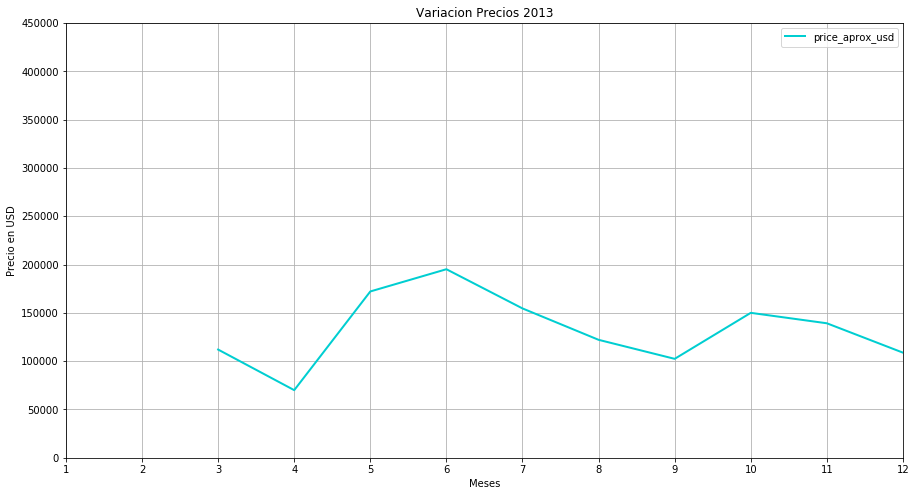
\includegraphics[width=6in, height=4.2in]{images/variacion2013}
		   	\end{center}
        		\begin{center}
       			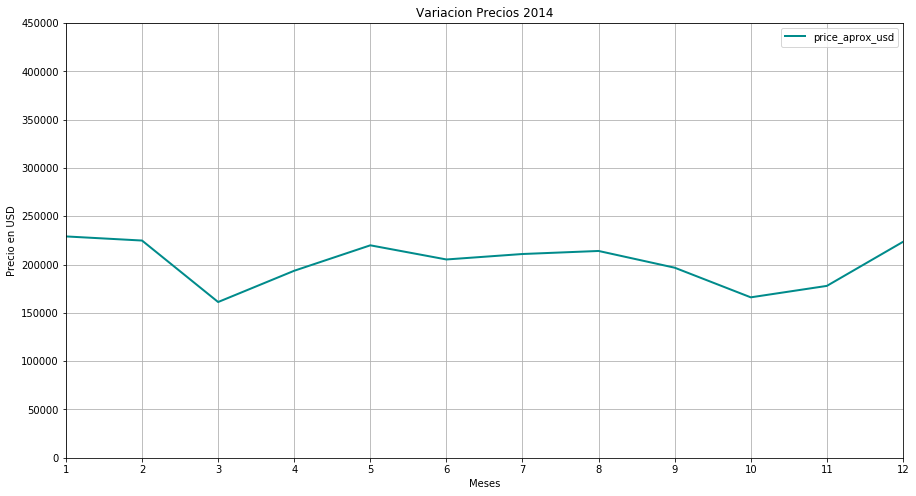
\includegraphics[width=6in, height=4.2in]{images/variacion2014}
		   	\end{center}
        		\begin{center}
       			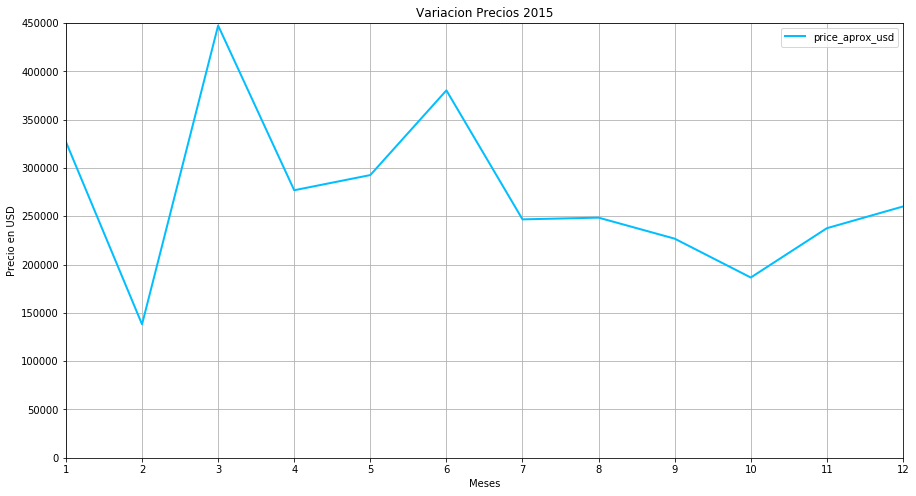
\includegraphics[width=6in, height=4.2in]{images/variacion2015}
		   	\end{center}
        		\begin{center}
       			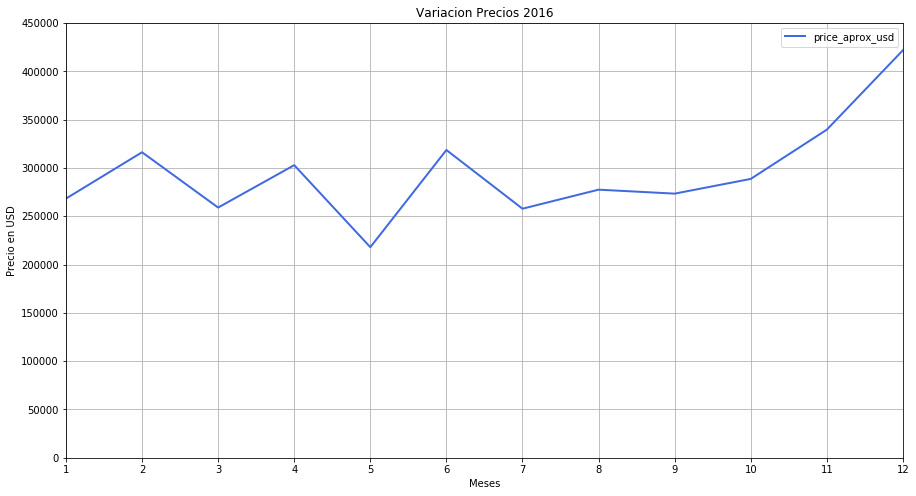
\includegraphics[width=6in, height=4.2in]{images/variacion2016}
		    \end{center}
        		\begin{center}
       			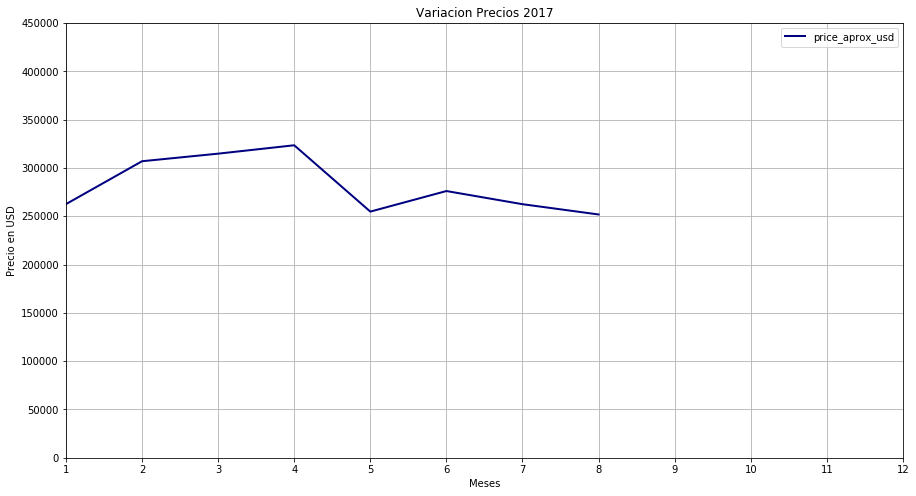
\includegraphics[width=6in, height=4.2in]{images/variacion2017}
		   	\end{center}

	      \subsection{Ubicación de las propiedades con mayor precio}
    			Luego de presentados los gráficos que representan la fluctuación del precio a través de los años, se procede a presentar
    			una serie de gráficos con el objetivo de analizar la ubicación de las propiedades con mayor precio. \\
 			\tab Para esto, se representa en distintos \code{Heats Map} la ubicación de las propiedades con mayor precio en cada año,
 			es decir que se filtro el mes que poseía un máximo en cada gráfico anterior y se representaron todas las propiedades que
 			estaban en dicho mes.
	        \begin{center}
    	         	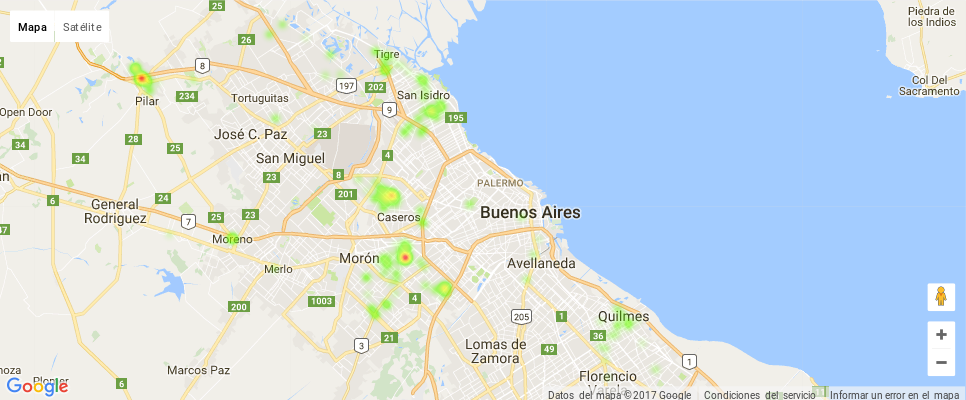
\includegraphics[width=7in, height=4in]{images/ubicP2013}
            		\textbf{Gráfico de las propiedades con mayor precio en el 2013.}
        		\end{center}
        		\begin{center}
              	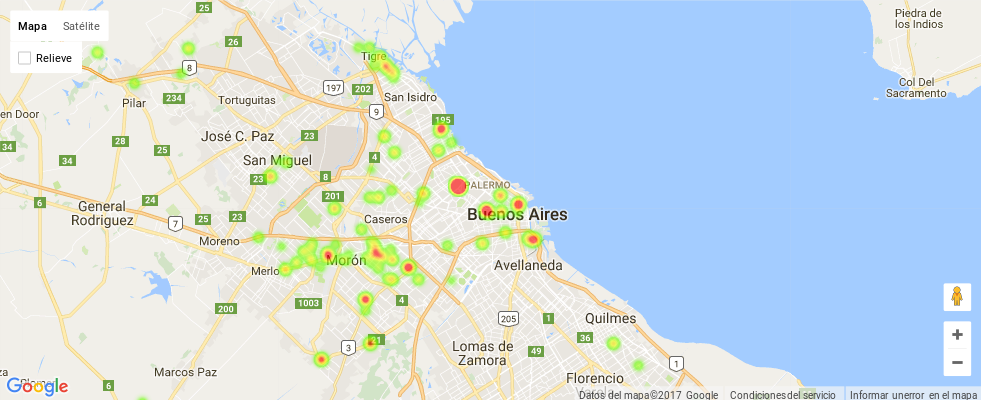
\includegraphics[width=7in, height=4in]{images/ubicP2014}
             	\textbf{Gráfico de las propiedades con mayor precio en el 2014.}
        		\end{center}
        		\begin{center}
             	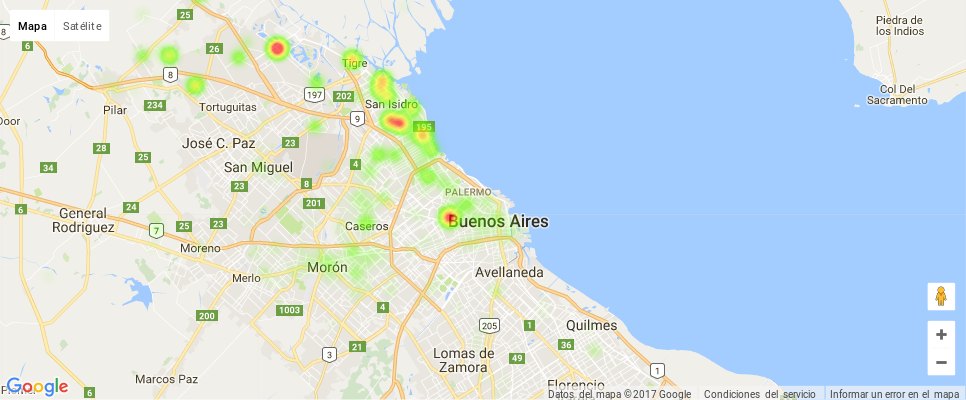
\includegraphics[width=7in, height=4in]{images/ubicP2015}
             	\textbf{Gráfico de las propiedades con mayor precio en el 2015.}
        		\end{center}
        		\begin{center}
              	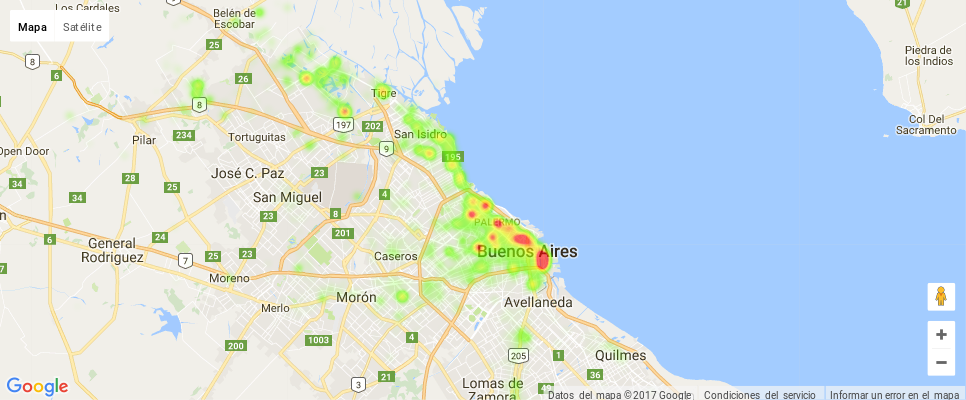
\includegraphics[width=7in, height=4in]{images/ubicP2016}
             	\textbf{Gráfico de las propiedades con mayor precio en el 2016.}
        		\end{center}
        		\begin{center}
              	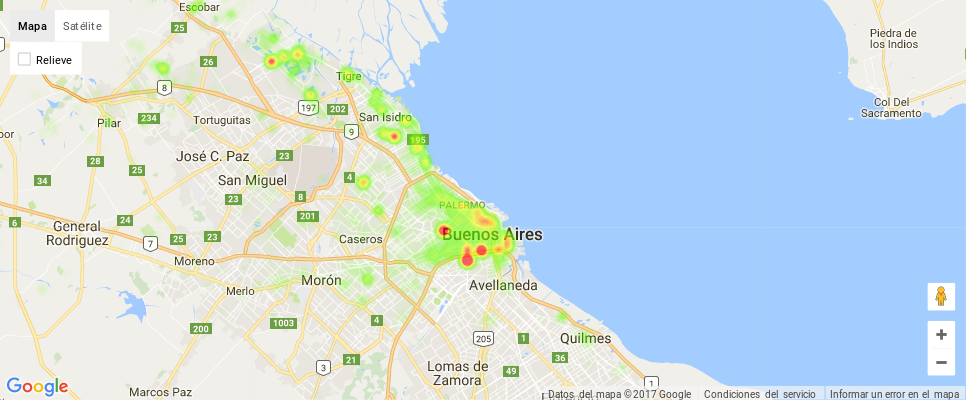
\includegraphics[width=7in, height=4in]{images/ubicP2017}
             	\textbf{Gráfico de las propiedades con mayor precio en el 2017.}
       		\end{center}
      	\subsection{Conclusiones de la Fluctuación del precio aproximado.}
			De los gráficos de promedios presentados anteriormente, se pueden visualizar rápidamente los meses con mayor y menor
			precio de propiedades en cada año. Se presenta una tabla con dichos datos:
        		\begin{center}
          		\begin{tabular}{ |c|c|c| }
            			\hline
		        		\multicolumn{3}{|c|}{Limites de precios por años.}\\
        		   		\hline
        		   		\hline
        		   		Año & Mes con Mayor Precio & Mes con menor Precio \\
        		   		\hline
        		   		2013 & Junio & Abril \\
        		   		2014 & Enero & Marzo \\
        		   		2015 & Marzo & Febrero \\
        		   		2016 & Diciembre & Mayo \\
        		   		2017 & Abril & Agosto \\
		            \hline
		        \end{tabular}
		    \end{center}
			\tab Cabe mencionar que estos son los datos que fueron filtrados para poder realizar los \code{Heats Map}. \\
	         \tab Por otra parte, se puede ver en la tabla presentada anteriormente que no se puede sugerir una tendencia de meses
	         con mayores-menores precios, ya que los resultados fueron muy variables. \\
	         \tab Con el objetivo de brindar otra mirada de la diferencia general entre los precios de distintos años, se construyó
	         otro gráfico que representa los mismo promedios anteriormente mencionados, pero organizados de distinta manera para
	         poder que puedan ser comparados entre distintos años. A continuación presentamos el gráfico:
			\begin{center}
              	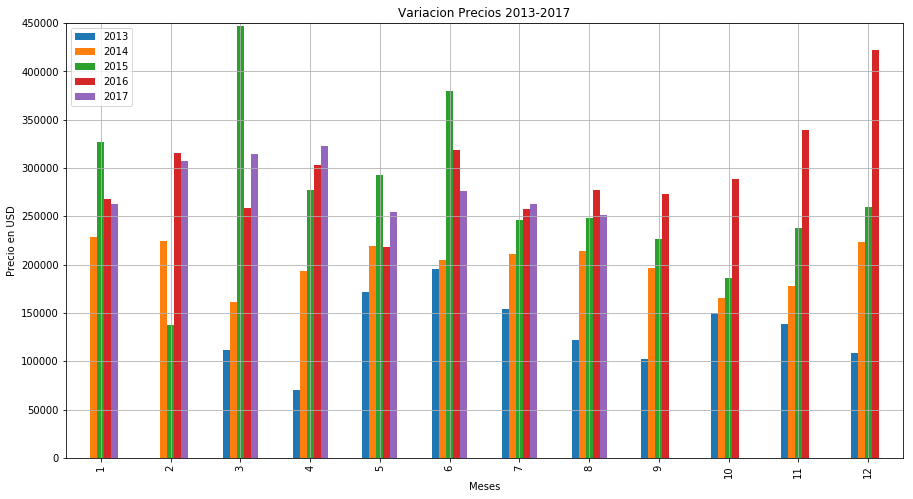
\includegraphics[width=6in, height=4.2in]{images/comparacionAnual}
        		\end{center}
        		\tab Como se menciono anteriormente, este gráfico tiene la finalidad de poder brindar una mirada global de los precios a
        		lo largo de los años. Como se puede ver, tenemos en el eje x los meses y para cada mes representamos los 5 años a
        		analizar. Observando detenidamente, se pueden extraer muchas conclusiones. \\
			\tab Lo primero y mas sencillo de ver son los meses con mayor y menor precio de los 5 años. Se puede observar que el 
			mes de Marzo del 2015 fue el que tuvo precios mas elevados de ventas, y por el contrario, el mes de Abril del 2013 
			fue el que tuvo los precios mas bajos en las mismas. Ademas se puede ver que 2013 tuvo menor precio que el resto de
			los años en todos los meses. Siguiendo la misma linea, es fácil observar que 2014 es el segundo año con menores precios,
			salvo en febrero que supero a 2015. De todas formas, se debe considerar que los años recientemente mencionados no son
			del todo representativos, ya que no se cuenta con la misma cantidad de datos que para los años posteriores.Por otro
			lado se puede visualizar que los primeros meses de 2015 fueron muy variantes, teniendo su mínimo en Febrero y máximo
			en Marzo, pero a partir de Junio-Julio se establece una media que supera a los 2 años anteriormente mencionados.
			Por último se puede ver que el año 2016 en la primera mitad posee precios que se sitúan entre los mas elevados, y
			en la segunda mitad establece una tendencia creciente la cual supera al resto de los años.
       		\tab A pesar de que los últimos años poseen un precio promedio mas elevado que los años previos, no se puede inferir
       		que haya aumentado el precio en el correr de los años, debido a la abrupta diferencia entre la cantidad de datos. De
       		todas formas, si solo es considerado el periodo 2015-2017, el cual posee la cantidad de entradas necesarias como para
       		ser representativo, obtenemos los siguientes resultados:
       		\begin{center}
       			\begin{tabular}{ |c|c| }
       			\hline
       			\multicolumn{2}{|c|}{Promedios Anuales de Precios.}\\
       			\hline
       			\hline
       			Año & Promedio(USD)\\
       			\hline
       			2015 & 292504 \\
       			2016 & 315746 \\
       			2017 & 275694 \\
       			\hline
	          	\end{tabular}
	      	\end{center}
     
			\tab De lo cual se puede ver rápidamente que el año 2016 fue el que tuvo precios mas elevados. De todas formas, hay
			que considerar que el año 2017 solo tiene entradas hasta agosto. \\
       		\tab Por otra parte, siguiendo el análisis recientemente hecho, se puede observar una cierta tendencia en los
       		\code{Heats Maps} presentados anteriormente. En dichos gráficos se puede notar que en los primeros años hay un
       		predominio de propiedades en \textit{Zona Norte} y \textit{Zona Oeste} del \textit{Gran Buenos Aires}. Esto puede
       		deberse, a la baja cantidad de entradas de dichos años, ya solo quedan las propiedades que no fueron vendidas.
       		Siguiendo con este análisis, se puede observar que los años posteriores poseen un mayor porcentaje de viviendas con
       		mayor precio en la zona de \textit{CABA}. Ademas, a esto le podemos sumar el análisis realizado en la sección 3.1,
       		sobre los barrios con mayor \code{Precio por m$^2$}. En ese análisis se obtuvo que los barrios con mayor valor de
       		metro cuadrado, están ubicados en \textit{CABA}, y mas precisamente, están ubicados en la zona que los últimos
       		2 \code{Heats Maps} nos indican mayor precio en las propiedades.
		\section{Conclusiones generales}
			Para finalizar esta parte, reflexionaremos sobre la información obtenida respecto del precio del $m^2$ en la Ciudad
			Autónoma de Buenos Aires y el Gran Buenos Aires. \\
			\tab Por empezar, es importante mencionar por qué esta es la parte uno; el precio del metro cuadrado será nuestra, por
			decir de alguna manera, \emph{unidad de medida} a lo largo de todo el trabajo. Por esta razón, parece correcto conocer
			cómo es que se distribuye en el espacio y cómo varió en los últimos años al inicio. \\
			\tab Conociendo la Ciudad de Buenos Aires y el momento actual del país, los resultados fueron los esperados. Es decir,
			la distribución espacial de los precios por $m^2$ es la esperada (disminuye a medida que nos alejamos de las conocidas
			'zonas caras' de la ciudad y describe a los llamados cordones del conurbano) y el precio en los últimos años tiene una
			tendencia creciente, tanto por $m^2$ como el precio total.
		\part{Análisis del tipo de las propiedades}
		En esta parte, se analizará como las distintas características de las propiedades son afectadas por el tipo de propiedad.
		Esto es, si son negocios, casas, PHs o departamentos.
		\section{Tipos de propiedades y sus superficies}
			La idea de esta sección es analizar en que lugares podemos encontrar a las propiedades con mayor y menor superficie
			en CABA y GBA. \\
			\tab Se debe mencionar que para realizar este análisis nos quedamos sólo con ciertos barrios en base a la cantidad de
			propiedades de cada tipo que contienen. Este recorte se realizó de la siguiente manera:
			\begin{center}
				\begin{tabular}{ |c|c|c| }
					\hline
					\multicolumn{2}{|c|}{Recorte de barrios}\\
					\hline
					\hline
					Tipo & Cantidad mínima \\
					\hline
					Casa & 35\\
					Locales & 15\\
					Departamentos & 180\\
					PHs & 40\\
					\hline
				\end{tabular}
			\end{center}
			\subsection{¿Dónde están las propiedades más grandes según su tipo?}
				\subsubsection{Casas}
					En el caso de las casas, al hacer un \emph{Top 5}, obtenemos el siguiente resultado:
					\begin{center}
						\begin{tabular}{ |c|c|c| }
							\hline
							\multicolumn{3}{|c|}{Superficie promedio de las casas por barrio}\\
							\hline
							\hline
							Puesto & Barrio & Superficie [$m^2$]\\
							\hline
							1 & Benavidez & 718 \\
							2 & Parque Leloir & 530 \\
							3 & Maschwitz & 499 \\
							4 & Acassuso & 481 \\
							5 & Belén de Escobar & 455\\
							\hline
						\end{tabular}
					\end{center}
					\tab Se puede ver que las casas en estos cinco barrios son considerablemente grandes y que el primero, Benavidez,
					tiene un promedio mucho mayor que el segundo ($26\%$ más grande) mientras que entre los siguientes cuatro barrios
					la diferencia es menor. A continuación, veremos un gráfico de barras de estos primeros 5 barrios.
					\begin{center}
   		    				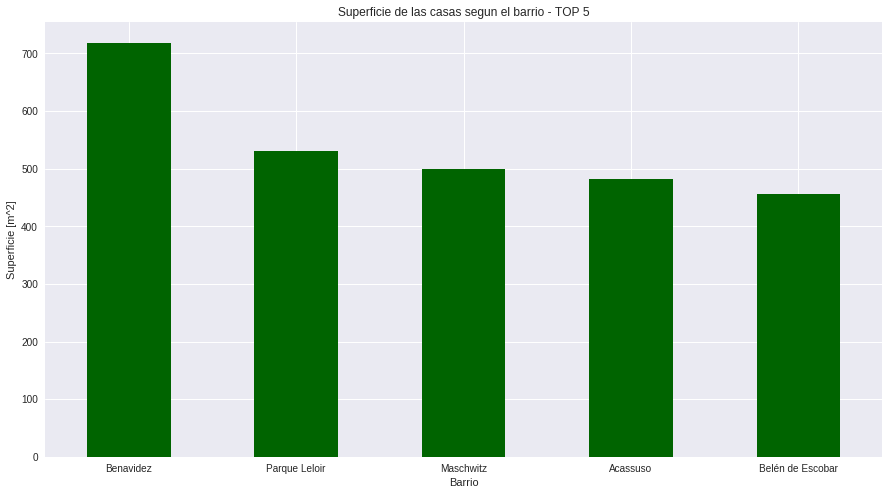
\includegraphics[width=\textwidth]{images/houseSurfaceTopBar}
				  	\end{center}
				  	\tab En este gráfico se ve lo mencionado previamente, una considerable diferencia entre el primero y el segundo
				  	y luego un descenso más estable. \\
				  	\tab Finalmente, veremos cuál es la ubicación geográfica de estas casas.
				  	\begin{center}
   		    				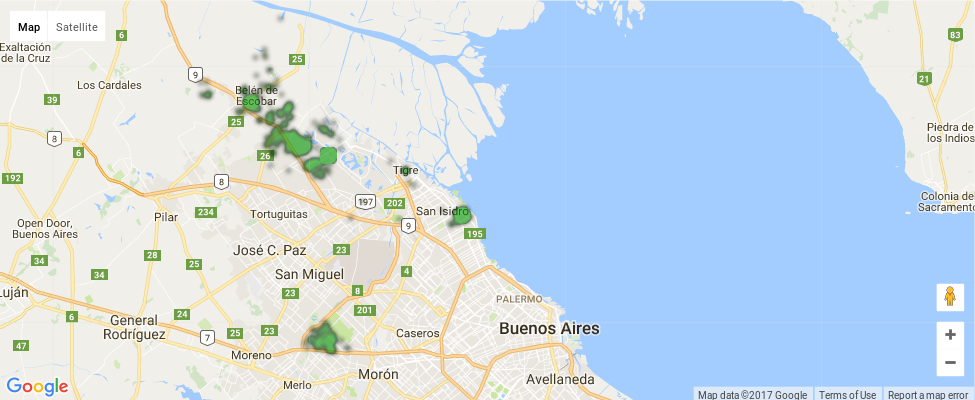
\includegraphics[width=\textwidth]{images/houseSurfaceTopMap}
				  	\end{center}
				  	\tab Se puede ver que, como era de esperar, son todos barrios alejados de la Capital Federal, principalmente en
				  	Zona Norte. \\
				  	\tab Podría decirse, entonces, que las casas más grandes se encuentran en la provincia de Buenos Aires. De todos
				  	modos, se espera encontrar barrios como Belgrano en los primeros puestos (en Belgrano R hay casas muy grandes) y,
				  	de hecho, es el décimo puesto.
				\subsubsection{PHs}
					Para los PHs, el \emph{Top 5} arroja los siguientes resultados:
					\begin{center}
						\begin{tabular}{ |c|c|c| }
							\hline
							\multicolumn{3}{|c|}{Superficie promedio de los PHs por barrio}\\
							\hline
							\hline
							Puesto & Barrio & Superficie [$m^2$]\\
							\hline
							1 & Caseros & 165\\
							2 & San Telmo & 160.4\\
							3 & Barracas & 159.9\\
							4 & Almagro & 142.7 \\
							5 & Ciudadela & 142.6\\
							\hline
						\end{tabular}
					\end{center}
					\tab En este caso vemos que la diferencia entre los primeros cinco barrios es muy pequeña, de hecho, entre el
					segundo y tercero y entre el cuarto y el quinto, la diferencia es menor de un metro cuadrado. Si vemos esto en
					un gráfico de barras:
					\begin{center}
   		    				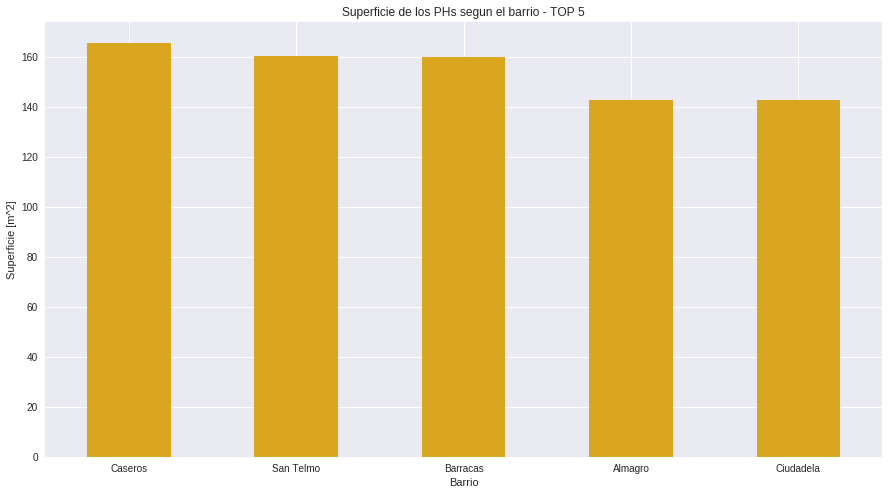
\includegraphics[width=\textwidth]{images/phSurfaceTopBar}
				  	\end{center}
				  	\tab Podemos ver la pequeña diferencia de superficie entre los primeros cinco barrios. Cabe destacar que la
				  	máxima superficie en este caso es el $23\%$ de la máxima superficie de las casas. \\
				  	\tab En cuanto a la ubicación geográfica de estos PHs, tenemos lo siguiente:
				  	\begin{center}
   		    				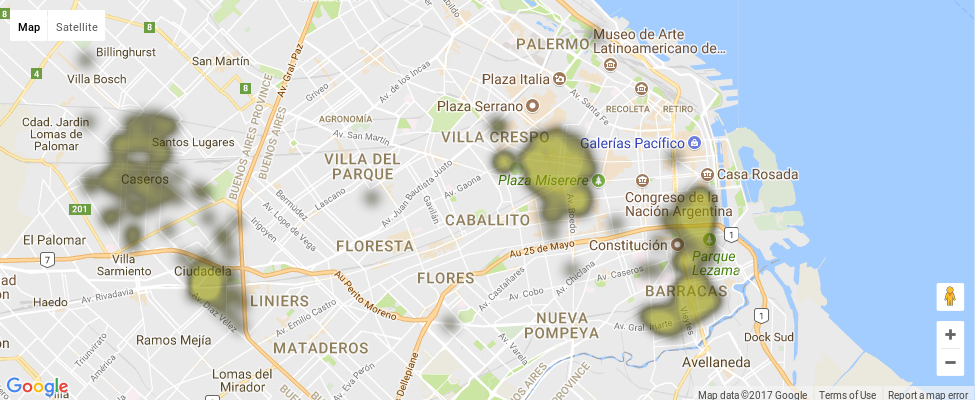
\includegraphics[width=\textwidth]{images/phSurfaceTopMap}
				  	\end{center}
				  	\tab Vemos que estos PHs se encuentran en Capital Federal y en dos barrios de la Provincia muy cercanos a CABA.
				  	Esto puede significar dos cosas; que simplemente los PHs más grandes están en la zona sur de CABA y algunos
				  	sectores de provincia o que es más común encontrar PHs en dichos lugares y no así en otros sectores de la ciudad,
				  	más alejados como con las casas, por lo que los primeros son los principales.
				\subsubsection{Departamentos}
					Para los primeros, el \emph{Top 5} es:
					\begin{center}
						\begin{tabular}{ |c|c|c| }
							\hline
							\multicolumn{3}{|c|}{Superficie promedio de los departamentos por barrio}\\
							\hline
							\hline
							Puesto & Barrio & Superficie [$m^2$]\\
							\hline
							1 & Palermo Chico & 177 \\
							2 & Puerto Madero & 150 \\
							3 & Retiro & 132 \\
							4 & Recoleta & 130\\
							5 & Barrio El Golf & 116\\
							\hline
						\end{tabular}
					\end{center}
					\tab Cabe destacar que en este caso no se unificaron los sectores de Palermo porque se consideró importante
					mostrar al barrio con los departamentos de mayor superficie promedio. \\
					\tab Al ver la tabla, encontramos cuatro barrios conocidos no solo como 'caros' en la Capital Federal sino
					también como el lugar de edificios grandes y lujosos, como es el caso de Puerto Madero y Retiro, por lo que
					no parece extraño encontrarlos en el \emph{Top 5}. El quinto puesto lo tiene un barrio cerrado de Tigre, donde
					también es de esperar que los departamentos sean grandes y lujosos. \\
					\tab El gráfico de barras en este caso nos muestra un descenso más abrupto que en el caso de los PHs y las casas.
					\begin{center}
   		    				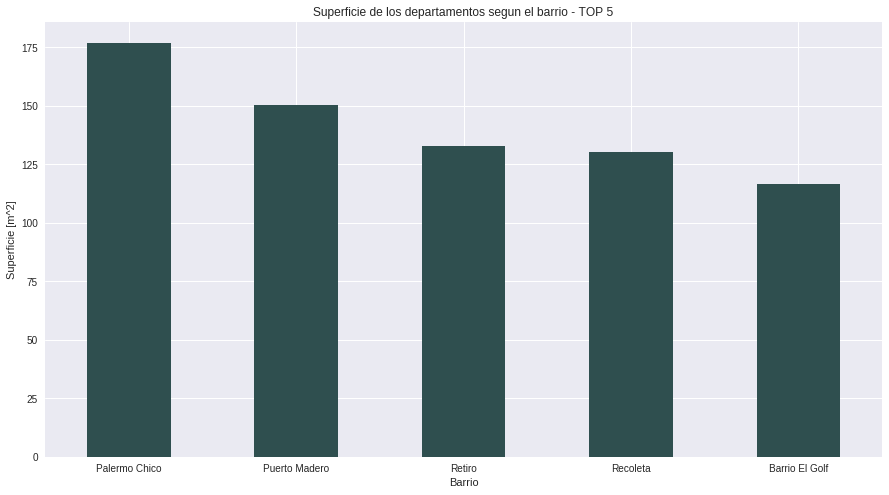
\includegraphics[width=\textwidth]{images/apartmentSurfaceTopBar}
				  	\end{center}
				  	\tab Vemos también que las superficies, en el caso de los máximos, son muy similares a las de los PHs (y por ende
				  	mucho menores que las de las casas). \\
				  	\tab Para la visualización de la ubicación geográfica no tuvimos en cuenta a el Barrio El Golf, pues por estar
				  	tan alejado de Capital Federal, no permite crear un gráfico entendible y útil.
				  	\begin{center}
   		    				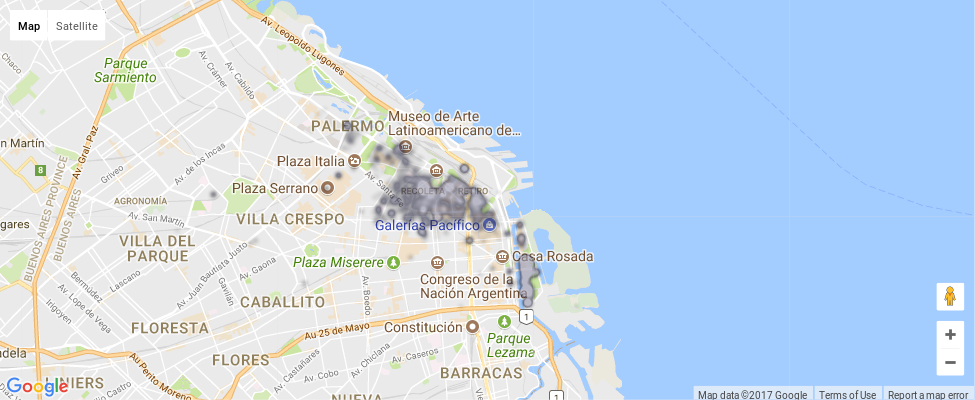
\includegraphics[width=\textwidth]{images/apartmentSurfaceTopMap}
				  	\end{center}
				  	\tab Vemos entonces que los departamentos con mayor superficie promedio se encuentran en aquellos barrios donde
				  	el precio por $m^2$ promedio también es el máximo. Esto se debe, como se dijo antes, a el 'alto nivel' de la
				  	zona, donde los edificios son lujosos y con muchos servicios y los departamentos suelen ser pisos o semi-pisos.
				\subsubsection{Locales}
					Finalmente, el \emph{Top 5} de los locales es el siguiente:
					\begin{center}
						\begin{tabular}{ |c|c|c| }
							\hline
							\multicolumn{3}{|c|}{Superficie promedio de los locales por barrio}\\
							\hline
							\hline
							Puesto & Barrio & Superficie [$m^2$]\\
							\hline
							1 & Martínez & 259\\
							2 & Caballito & 232\\
							3 & Balvanera & 231\\
							4 & San Telmo & 219\\
							5 & Microcentro & 217\\
							\hline
						\end{tabular}
					\end{center}
					\tab Aquí nos encontramos con un primer puesto no esperado. Pues si bien Martínez tiene una zona comercial, no
					se esperaba que fuera el que tiene los locales más grandes en promedio. Por otro lado, la aparición de los
					barrios céntricos no nos sorprende, dado que allí hay un polo comercial muy importante y con locales de gran
					superficie. De todas formas, más adelante analizaremos los barrios en los que hay mayor cantidad de locales (o
					de cada tipo de propiedad, mejor dicho). \\
					\tab Si vemos el gráfico de barras:
					\begin{center}
   		    				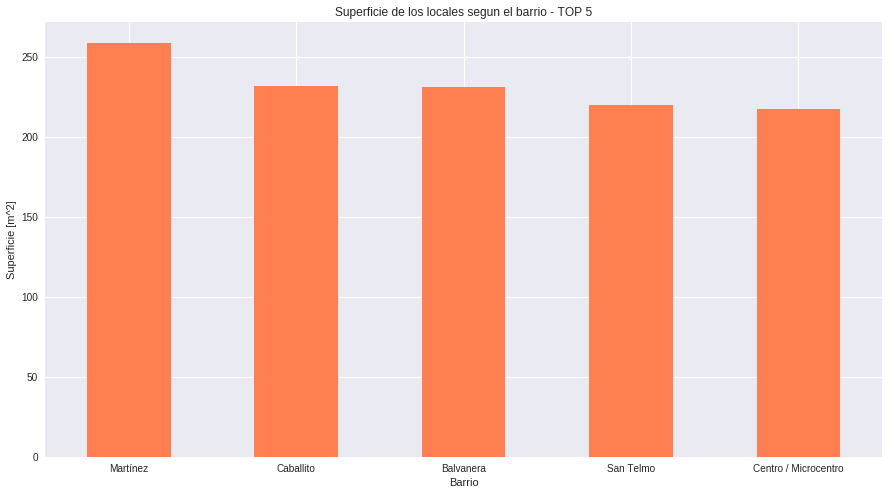
\includegraphics[width=\textwidth]{images/storeSurfaceTopBar}
				  	\end{center}
				  	\tab Vemos que la diferencia entre los primeros cinco barrios es pequeña y que, en promedio, los locales son
				  	más grandes que los departamentos y PHs, al analizar a los cinco más grandes de cada uno. \\
				  	\tab En cuanto a la ubicación geográfica:
				  	\begin{center}
   		    				\includegraphics[width=\textwidth]{images/storeSurfaceTopMap}
				  	\end{center}
				  	\tab Vemos que, como dijimos previamente, hay una gran cantidad en la zona céntrica de la ciudad mientras que
				  	también aparece el barrio de Martínez en Zona Norte y Caballito en el centro-sur geográfico de CABA.
			\subsection{¿Dónde están las propiedades más chicas según su tipo?}

        \subsubsection{Casas}
          Para las casas, el \emph{Bottom 5} está compuesto por los siguientes barrios:
          \begin{center}
            \begin{tabular}{ |c|c|c| }
              \hline
              \multicolumn{3}{|c|}{Superficie promedio de las casas por barrio}\\
              \hline
              \hline
              Puesto & Barrio & Superficie [$m^2$]\\
              \hline
              5 & José León Suarez & 176\\
              4 & Remedios de Escalada & 175\\
              3 & Lanús & 173\\
              2 & Munro & 161 \\
              1 & Llavallol & 160\\
              \hline
            \end{tabular}
          \end{center}
          \tab Aquí podemos ver que incluso el barrio con el promedio más pequeño tiene una superficie promedio mayor
          a la de los barrios con mayor superficie promedio en el caso de los PHs y los departamentos. \\
          \tab Si se grafican estos cinco barrios:
          \begin{center}
                  \includegraphics[width=\textwidth]{images/houseSurfaceBottomBar}
            \end{center}
            \tab Se puede ver la poca diferencia que hay entre cada uno de los barrios, siendo entre los cinco de sólo
            $16m^2$ mientras que entre los primeros tres hay sólo $3m^2$ de diferencia. \\
            \tab En cuanto a la ubicación geográfica de estos barrios, podemos ver el siguiente mapa:
            \begin{center}
                  \includegraphics[width=\textwidth]{images/houseSurfaceBottomMap}
            \end{center}
            \tab Aquí se observa que los barrios con menor promedio de superficie para las casas, al igual que ellos con
            mayor promedio, se encuentra en la provincia de Buenos Aires, divido entre el sur y el norte. Tanto para el
            sur como para el norte podemos ver que, salvo por Munro, no son barrios del primer cordón del conurbano sino
            del segundo. Es decir, al igual que en el Top 5, encontramos las casas con menor superficie en lugares alejados
            de la Capital Federal (aunque en este caso más cercanos que en el anterior).
        \subsubsection{PHs}
          En el caso de los PHs, tenemos un \emph{Bottom 5} de la siguiente forma:
          \begin{center}
            \begin{tabular}{ |c|c|c| }
              \hline
              \multicolumn{3}{|c|}{Superficie promedio de los PHs por barrio}\\
              \hline
              \hline
              Puesto & Barrio & Superficie [$m^2$]\\
              \hline
              5 & Saavedra & 89\\
              4 & Lanús & 87\\
              3 & Beccar & 87\\
              2 & Quilmes & 82\\
              1 & Parque Chacabuco & 79\\
              \hline
            \end{tabular}
          \end{center}
          \tab Aquí, nuevamente vemos una diferencia muy pequeña entre el quinto y el primero. Vemos que se repite Lanús,
          por lo que podríamos comenzar a suponer que es un barrio donde las propiedades tienden a ser pequeñas. \\
          \tab Si analizamos la tabla con un gráfico de barras, nuevamente veremos una diferencia entre barrios muy
          pequeña. De hecho, Lanús y Beccar comparten el mismo valor.
          \begin{center}
                  \includegraphics[width=\textwidth]{images/phSurfaceBottomBar}
            \end{center}
            \tab En cuanto a la ubicación geográfica, veremos una ubicación de los barrios muy variada:
            \begin{center}
                  \includegraphics[width=\textwidth]{images/phSurfaceBottomMap}
            \end{center}
            \tab Desde Saavedra y Parque Chacabuco en CABA, hasta dos barrios alejados como Beccar en Zona Norte y Quilmes
            en Zona Sur.
        \subsubsection{Departamentos}
          El \emph{Bottom 5} de los departamentos está conformado por:
          \begin{center}
            \begin{tabular}{ |c|c|c| }
              \hline
              \multicolumn{3}{|c|}{Superficie promedio de los departamentos por barrio}\\
              \hline
              \hline
              Puesto & Barrio & Superficie [$m^2$]\\
              \hline
              5 & Munro & 50\\
              4 & Villa Luzuriaga & 48\\
              3 & Morón & 48\\
              2 & Parque Chas & 46\\
              1 & Boedo & 40\\
              \hline
            \end{tabular}
          \end{center}
          \tab La superficie promedio para estos departamentos es de aproximadamente la mitad de los PHs más pequeños
          y tienen un promedio menor al $30\%$ de los departamentos más grandes. Aquí encontramos nuevamente a Munro, que
          también se encuentra en el \emph{Bottom 5} de las casas. \\
          \tab Aquí, nuevamente, un gráfico de barras nos dará cinco barras muy similares, con Villa Luzuriaga y Morón
          compartiendo el mismo valor y una diferencia entre el primero y el quinto de sólo  $10m^2$.
          \begin{center}
                  \includegraphics[width=\textwidth]{images/apartmentSurfaceBottomBar}
            \end{center}
            \tab En cuanto a la ubicación geográfica, si observamos el siguiente mapa:
            \begin{center}
                  \includegraphics[width=\textwidth]{images/apartmentSurfaceBottomMap}
            \end{center}
            \tab Podemos ver que no hay una tendencia particular, pues encontramos barrios dentro de Capital Federal, en la
            Zona Norte y en la Zona Oeste, siendo dos los barrios de la última y dos los de la primera.
        \subsubsection{Locales}
          Finalmente, para los locales, el \emph{Bottom 5} es el siguiente:
          \begin{center}
            \begin{tabular}{ |c|c|c| }
              \hline
              \multicolumn{3}{|c|}{Superficie promedio de los locales por barrio}\\
              \hline
              \hline
              Puesto & Barrio & Superficie [$m^2$]\\
              \hline
              5 & Palermo & 145\\
              4 & Ramos Mejía & 125\\
              3 & Villa Crespo & 120\\
              2 & Barrio Norte & 119\\
              1 & Belgrano & 92\\
              \hline
            \end{tabular}
          \end{center}
          \tab Esta tabla nos permite ver que entre los integrantes del \emph{Bottom 5} y los del \emph{Top 5} hay una
          variación del $42\%$, que es la más pequeña entre todos los tipos. \\
          \tab El hecho de que Belgrano sea el más pequeño se lo atribuímos a la cantidad de locales que se pueden
          encontrar en dicho barrio tanto en avenidas como Cabildo o en galerías comerciales en esa misma avenida, en donde
          se encuentran muchísimos locales muy pequeños uno al lado del otro.
          \tab En este caso, el gráfico de barras si mostrará una variación importante, pues Belgrano tiene una
          superficie promedio que representa el $63\%$ de la de Palermo.
          \begin{center}
                  \includegraphics[width=\textwidth]{images/storeSurfaceBottomBar}
            \end{center}
            \tab Finalmente, si analizamos la ubicación geográfica de estos barrios, vemos lo siguiente:
            \begin{center}
                  \includegraphics[width=\textwidth]{images/storeSurfaceBottomMap}
            \end{center}
            \tab La mayoría de los barrios se encuentran en una zona casi continua del Centro-Norte de Capital Federal con
            la excepcion de Ramos Mejía en Zona Oeste. \\
            \tab Se puede observar, si se compara con el \emph{Top 5}, se puede ver que los barrios en este último se
            encuentran 'de Recoleta para el Sur' y en el caso actual se encuentran 'de Recoleta para el Norte'.

		\section{Tipos de propiedades y sus precios}
			\subsection{¿Dónde están las propiedades más caras según su tipo?}
				El objetivo de esta sección es analizar donde se ubican las propiedades mas caras, dependiendo del tipo que sean. \\
				Vale destacar, que para realizar el análisis próximo a presentarse, primero se filtro por tipo de propiedad y luego se agrupo por barrio, dejando el promedio y la cantidad de entradas como valor. Para todos los casos a presentarse a continuación, se filtro con un mínimo de entradas igual a 20.

				\subsubsection{Casas}
				Para el caso particular de las casas, se realizo un \emph{TOP 5} obteniendo los siguientes resultados:

					\begin{center}
						\begin{tabular}{ |c|c| }
							\hline
							\multicolumn{2}{|c|}{TOP 5 de las casas mas caras}\\
							\hline
							\hline
							Barrio & Precio(USD)\\
							\hline
							 Belgrano & 2610.771984 \\
							 Palermo & 2598.033402 \\
							 Santa Barbara Barrio Cerrado & 2418.894358 \\
							 Nuñez & 2270.098719 \\
							 Barrio Los Castores & 2223.561320 \\
							\hline
						\end{tabular}
					\end{center}

				Se puede observar en la tabla, que la diferencia entre los primeros 2 barrios es muy pequeña, pero aumenta a mas de 1000 Usd con los últimos 3 de la tabla.

				\begin{center}
   		    				\includegraphics[width=\textwidth]{images/topCc}
				\end{center}

				Finalmente, se añade la ubicación de dichas casas:

				\begin{center}
   		    				\includegraphics[width=\textwidth]{images/ubicCc}
				\end{center}

				Entonces se puede notar que las casas mas caras, como se analizo en el capitulo anterior, se encuentran en las zonas donde tanto el precio por metro cuadrado, como el precio aproximado de las viviendas es mas elevado, salvo por el Barrio Santa Barbara. Este último, es un barrio cerrado ubicado en Benavidez.


				\subsubsection{PHs}
				Para los PHs el \emph{TOP 5}, entrego los siguientes resultados:

					\begin{center}
						\begin{tabular}{ |c|c| }
							\hline
							\multicolumn{2}{|c|}{TOP 5 de las PHs mas caros}\\
							\hline
							\hline
							Barrio & Precio(USD)\\
							\hline
							Palermo Soho & 2657.484915 \\
							Coghlan & 2485.627732 \\
							Belgrano & 2435.721287 \\
							Palermo & 2382.434241 \\
							Nuñez & 2275.340938 \\
							\hline
						\end{tabular}
					\end{center}

				\begin{center}
   		    				\includegraphics[width=\textwidth]{images/topPHc}
				\end{center}

				Tal como se puede ver en el gráfico y en la tabla, la mayor diferencia se presenta entre el primero y el segundo, siendo esta de 172 Usd.\\
				Finalmente, se añade la ubicación de dichos PH:

				\begin{center}
   		    				\includegraphics[width=\textwidth]{images/ubicPHc}
				\end{center}

				Si bien los datos son consistentes respecto con el análisis hecho en el capitulo anterior, uno esperaría que la mayor cantidad de PHs se ubicara en GBA. Como podemos ver, esta hipótesis no es valida.

				\subsubsection{Departamentos}
				Para los Departamentos el \emph{TOP 5}, arrojo los siguientes resultados:

					\begin{center}
						\begin{tabular}{ |c|c| }
							\hline
							\multicolumn{2}{|c|}{TOP 5 de las Departamentos mas caros}\\
							\hline
							\hline
							Barrio & Precio(USD)\\
							\hline
							Puerto Madero & 5681.950867 \\
							Palermo Chico & 4372.664773 \\
							Las Cañitas & 3625.253679 \\
							Vicente López & 3365.357986 \\
							Olivos & 3307.502819 \\
							\hline
						\end{tabular}
					\end{center}

				\begin{center}
   		    				\includegraphics[width=\textwidth]{images/topDc}
				\end{center}

				Se puede observar claramente en el gráfico que, hay una diferencia muy abrupta entre las primeras 3 ubicaciones, estabilizándose hacia el final de la tabla.\\
				Finalmente, se añade la ubicación de dichos Departamentos:

				\begin{center}
   		    				\includegraphics[width=\textwidth]{images/ubicDc}
				\end{center}

				Como se puede observar en el gráfico anterior, se tiene la mayor cantidad departamentos con precio elevado en CABA. También hay que notar, que los departamentos que están en GBA se encuentran en barrios cercanos a CABA.

				\subsubsection{Locales}

					Para los Locales se obtuvieron los siguientes resultados del \emph{TOP 5}:

					\begin{center}
						\begin{tabular}{ |c|c| }
							\hline
							\multicolumn{2}{|c|}{TOP 5 de las Locales mas caros}\\
							\hline
							\hline
							Barrio & Precio(USD)\\
							\hline
							Palermo & 3944.669361 \\
							Recoleta & 3851.392729 \\
							Belgrano & 3361.595914 \\
							Villa Crespo & 3280.676456 \\
							Ramos Mejía & 3167.439625 \\
							\hline
						\end{tabular}
					\end{center}

				\begin{center}
   		    				\includegraphics[width=\textwidth]{images/topLc}
				\end{center}

				Se puede ver en la tabla y el gráfico, que la mayor diferencia se presenta entre los primeros 2 y los últimos 3.\\
				Finalmente, se añade la ubicación de los Locales mas caros:

				\begin{center}
   		    				\includegraphics[width=\textwidth]{images/ubicLc}
				\end{center}

				Como se puede observar en el gráfico anterior, los locales mas caros se concentran en CABA, salvo por los últimos 2 datos de la tabla.


			\subsection{¿Dónde están las propiedades más baratas según su tipo?}
				En esta sección se propone analizar donde se ubican las propiedades mas baratas. \\
				En dicha sección se realizaron los mismos filtrados que para las propiedades mas caras.

				\subsubsection{Casas}

				Se realizo un \emph{TOP 5} obteniendo los siguientes resultados para las casas:

					\begin{center}
						\begin{tabular}{ |c|c| }
							\hline
							\multicolumn{2}{|c|}{TOP 5 de las casas mas baratos}\\
							\hline
							\hline
							Barrio & Precio(USD)\\
							\hline
							Villa Udaondo & 864.062761 \\
							Valentín Alsina 	& 863.197187 \\
							Villa Madero & 862.186426 \\
							San Martín & 830.209696 \\
							La Tablada & 807.027363 \\
							\hline
						\end{tabular}
					\end{center}


				\begin{center}
   		    				\includegraphics[width=\textwidth]{images/topCb}
				\end{center}

				Se puede observar, que la diferencia entre los distintos barrios es muy pequeña. Dicha diferencia, no supera los 60 Usd entre el primero y el último.
				Finalmente, se añade la ubicación de dichas casas:

				\begin{center}
   		    				\includegraphics[width=\textwidth]{images/ubicCb}
				\end{center}

				Se puede notar, que las casas con menores precios se ubican en GBA, lo cual era esperable, ya que concuerda con el análisis de precio por metro cuadrado y de precio aproximado.

				\subsubsection{PHs}

					Para los PHs el se obtuvieron los siguientes resultados del \emph{TOP 5}:

					\begin{center}
						\begin{tabular}{ |c|c| }
							\hline
							\multicolumn{2}{|c|}{TOP 5 de las PHs mas baratos}\\
							\hline
							\hline
							Barrio & Precio(USD)\\
							\hline
							Villa Bosch & 1157.563280 \\
							Lanús Oeste & 1109.922068 \\
							El Palomar & 1103.662526 \\
							Ituzaingó & 1021.952671 \\
							San Martín & 947.012756 \\

							\hline
						\end{tabular}
					\end{center}

				\begin{center}
   		    				\includegraphics[width=\textwidth]{images/topPHb}
				\end{center}

				Se puede observar que se obtienen diferencias muy cercanas entre las distintas zonas, salvo entre la segunda y tercera donde la diferencia es mucho menor al resto de la tabla.

				\begin{center}
   		    				\includegraphics[width=\textwidth]{images/ubicPHb}
				\end{center}

				Como se puede ver en este gráfico, los resultados son totalmente esperables, ya que los PHs con menor precio se encuentran ubicados en \code{CABA}

				\subsubsection{Departamentos}

					Para los Departamentos el \emph{TOP 5}, entrego los siguientes resultados:

					\begin{center}
						\begin{tabular}{ |c|c| }
							\hline
							\multicolumn{2}{|c|}{TOP 5 de las Departamentos mas baratos}\\
							\hline
							\hline
							Barrio & Precio(USD)\\
							\hline
							Pompeya & 1205.936453 \\
							Bs.As. G.B.A. Zona Oeste & 1173.854686 \\
							Hurlingham & 1144.014297 \\
							Pilar Village & 1131.876143 \\
							José C Paz & 1057.673806 \\
						\end{tabular}
					\end{center}


				\begin{center}
   		    				\includegraphics[width=\textwidth]{images/topDb}
				\end{center}

				Se puede apreciar que las diferencias entre los barrios de la tabla, son muy parecidas entre sí.\\
				Finalmente, se añade la ubicación de dichos Departamentos:

				\begin{center}
   		    				\includegraphics[width=\textwidth]{images/ubicDb}
				\end{center}

				Se puede observar en el gráfico, que los departamentos con menores precios están ubicados únicamente en GBA. Lo cual es esperable, debido al análisis realizado en el capitulo anterior y lo obtenido con los departamentos mas caros.

				\subsubsection{Locales}

					Para los Locales el \emph{TOP 5} lanzo los siguientes resultados:

					\begin{center}
						\begin{tabular}{ |c|c| }
							\hline
							\multicolumn{2}{|c|}{TOP 5 de las Locales mas baratos}\\
							\hline
							\hline
							Barrio & Precio(USD)\\
							\hline
							San Justo & 1575.904794 \\
							Mataderos & 1544.208404 \\
							Temperley & 1509.434793 \\
							General San Martín & 1478.113426 \\
							Villa Ballester 	& 1264.444924 \\
							\hline
						\end{tabular}
					\end{center}

				\begin{center}
   		    				\includegraphics[width=\textwidth]{images/topLb}
				\end{center}

				Se puede ver que la mayor diferencia de precios entre las distintas localidades, se da entre las últimas 2 de la tabla, siendo las diferencias del resto muy similares.\\
				Finalmente, se añade la ubicación de los Locales mas baratos:

				\begin{center}
   		    				\includegraphics[width=\textwidth]{images/ubicLb}
				\end{center}

				Como era de esperar, los Locales mas baratos se encuentran ubicados en la zona de CABA.


		\section{Tipos de propiedades y sus ubicaciones}
			\subsection{¿En qué lugar hay más propiedades de cada tipo?}
				En esta sección se pretende analizar, las localidades que tienen mayor cantidad de propiedades de cada tipo.\\
				Vale aclarar que cada tipo de propiedad, fue filtrada por el siguiente rango de precios:

				\begin{center}
						\begin{tabular}{ |c|c|c| }
							\hline
							\multicolumn{3}{|c|}{Rango de precios Minímo y Maxímo}\\
							\hline
							\hline
							Tipo & Minímo(Usd) & Maxímo(Usd)\\
							\hline
							Casa & 150000 & 10000000\\
							Departamento & 90000 &300000\\
							Ph & 85000 & 1000000\\
							Locales & 150000 & 10000000\\
							\hline
						\end{tabular}
					\end{center}
				Por ultimo, también se pidió un mínimo de 20 entradas.

				\subsubsection{Casas}

				Aquí se analizara el resultado que se obtuvo a partir del \emph{TOP 5} de los barrios donde hay mas casas:

				\begin{center}
						\begin{tabular}{ |c|c| }
							\hline
							\multicolumn{2}{|c|}{TOP 5 de los barrios con mas casas}\\
							\hline
							\hline
							Barrio & Cantidad\\
							\hline
							Tigre & 1657.0 \\ 
							Benavidez & 1237.0 \\
							Pilar & 1219.0 \\ 
							Capital Federal & 921.0 \\
							Escobar & 700.0 \\
							\hline
						\end{tabular}
					\end{center}

				Además se agrega un gráfico con las ubicaciones de dichas casas:

				\begin{center}
   		    				\includegraphics[width=\textwidth]{images/ubicMasCasas}
				\end{center}

				Como se puede observar, la ubicación de los barrios con mas casas, esta prácticamente centralizada en CABA. Lo que uno esperaba, es que se hubiese centralizado sobre GBA, por el nivel de urbanización de CABA. Se ve con los gráficos y tablas, que esta hipótesis no es correcta.

				\subsubsection{PHs}

				El objetivo de esta sección es analizar los barrios con mayor cantidad de PHs. Se vera a continuación una tabla del top 5:

				\begin{center}
						\begin{tabular}{ |c|c| }
							\hline
							\multicolumn{2}{|c|}{TOP 5 de los barrios con mas PHs}\\
							\hline
							\hline
							Barrio & Cantidad\\
							\hline
							Ramos Mejía & 176.0 \\
							Palermo & 95.0 \\
							Mataderos &	91.0 \\
							Almagro & 84.0 \\
							Villa Crespo & 79.0 \\
							\hline
						\end{tabular}
					\end{center}

				Ahora se pasara a presentar un gráfico con las ubicaciones de los barrios con mayor cantidad de PHs:
				\begin{center}
   		    				\includegraphics[width=\textwidth]{images/ubicMPH}
				\end{center}

				Como se puede observar, los barrios con mayor cantidades de PHs, estan divididos entre CABA y Zona Oeste.

				\subsubsection{Departamentos}

				Dicha sección se presenta con el objetivo de analizar cuales son los barrios que tienen mayor cantidad de departamentos:

				\begin{center}
						\begin{tabular}{ |c|c| }
							\hline
							\multicolumn{2}{|c|}{TOP 5 de los barrios con mas Departamentos}\\
							\hline
							\hline
							Barrio & Cantidad\\
							\hline
							Belgrano & 1534.0 \\
							Palermo & 1440.0 \\
							Caballito &	1402.0 \\
							Tigre &	1232.0 \\
							Nordelta & 979.0 \\
							\hline
						\end{tabular}
					\end{center}

				A continuación se presentara un gráfico con las ubicaciones de dichos datos:

				\begin{center}
   		    				\includegraphics[width=\textwidth]{images/ubicMDeptos}
				\end{center}

				Como se puede ver, dicho gráfico esta centralizado en CABA y en Zona Norte, mas precisamente Tigre. La centralización que se da en CABA es totalmente esperable, por el nivel de urbanización de dichos lugares. De todas formas, uno esperaría que este todo centralizado en CABA, y como se puede ver no es de tal forma.

				\subsubsection{Locales}

				Esta sección se presenta con el objetivo de hacer un análisis similar a los anteriores, para los Locales:

				\begin{center}
						\begin{tabular}{ |c|c| }
							\hline
							\multicolumn{2}{|c|}{TOP 5 de los barrios con mas Departamentos}\\
							\hline
							\hline
							Barrio & Cantidad\\
							\hline
							Palermo & 113.0 \\
							Recoleta & 76.0 \\
							Villa Crespo & 71.0 \\
							Centro / Microcentro & 63.0 \\
							San Telmo &	55.0 \\
							\hline
						\end{tabular}
					\end{center}

				Ahora se presenta un gráfico con las ubicaciones:

				\begin{center}
   		    				\includegraphics[width=\textwidth]{images/ubicMLocales}
				\end{center}

				Como se puede observar, dicho gráfico presenta centralización en la zona de CABA.
				Esto es totalmente esperable, ya que los locales se encuentran cerca de muchos espacios verdes, o zonas donde se concentran las redes de transporte.

		\section{Variación del precio total a través de los años}
			%Al igual que en el análisis global de las propiedades, se presentaran gráficos que representan los promedios
%mensuales de las propiedades de tipo casa para cada año. En los siguientes gráficos, al igual que en el análisis
%global, el eje x representa los meses de cada año, y el eje y representa el precio de las propiedades en usd. Dicho
%precio varia entre 0−600000 usd.

			Esta sección tiene el objetivo de realizar un análisis de como variaron los precios de cada tipo de propiedad a lo largo de los años.\\
			Vale aclarar, que el año 2013 no se tuvo en cuenta ya que al dividir por tipos de propiedades quedaban muy pocas entradas de cada tipo.
			Por último, se aclara que los precios fueron recortados según la tabla de la sección anterior.

			\subsection{Casas}

			Aquí se pretende analizar la variación de los precios promedios de las casas entre los años 2014-2017. Con este fin, se presentaran gráficos que representan los promedios mensuales de las propiedades de tipo casa para cada año. En los siguientes gráficos, el eje x representa los meses de cada año, y el eje y representa el precio de las propiedades en usd. Dicho
precio varia entre 0 y 600000 usd.

			\begin{center}
   		    		\includegraphics[width=\textwidth]{images/vCasa2014}
			\end{center}

			\begin{center}
   		    		\includegraphics[width=\textwidth]{images/vCasa2015}
			\end{center}

			\begin{center}
   		    		\includegraphics[width=\textwidth]{images/vCasa2016}
			\end{center}

			\begin{center}
   		    		\includegraphics[width=\textwidth]{images/vCasa2017}
			\end{center}

			Como se puede observar, los gráficos promedios de la variación de precio de las casas siguen 				una tendencia similar a la analizada globalmente, en la sección 1. Algo importante a destacar, 				es el cambio brusco de los precios entre los meses Febrero-Marzo del año 2015. Al igual que en 				el análisis global, estos son los meses con menores y mayores precios de casas vendidas del año 			2015 respectivamente. Entonces se atribuye esta fluctuación a las casas, ya que como se vera 				mas adelante, no se presenta en el resto de las propiedades.
			\\
			Por ultimo se puede ver que el año 2016, fue un año muy estable con respecto a los precios 					promedios de las casas. Se ve en dicho gráfico que se establece una media que varia entre 350 y 			400 mil usd, a partir de la cual la fluctuación de ese año es muy pequeña.

			\subsection{PHs}


			Esta sección tiene el objetivo de analizar la variación de los precios promedios de los PH en el periodo que comprende los años 2014-2017. Para obtener una mirada generalizada de dicho periodo, se presentaran gráficos que representan los promedios mensuales de los PHs, al igual que en el caso anterior con las casas. En los gráficos a presentarse a continuación, los ejes poseen el mismo significado que en el caso anterior, con un maxímo para el eje y de 300000 usd.

			\begin{center}
   		    		\includegraphics[width=\textwidth]{images/vPH2014}
			\end{center}

			\begin{center}
   		    		\includegraphics[width=\textwidth]{images/vPH2015}
			\end{center}

			\begin{center}
   		    		\includegraphics[width=\textwidth]{images/vPH2016}
			\end{center}

			\begin{center}
   		    		\includegraphics[width=\textwidth]{images/vPH2017}
			\end{center}

			Como se puede notar, en los primeros 2 años los gráficos promedios poseen una notoria variación de los precios. Se puede ver que en el mes de Marzo de 2014, no se tienen entradas, y que la variación entre Enero-Junio los precios fue muy grande. Como se menciono en el análisis global, eso no quiere decir que hayan aumentado o disminuido los precios, sino que puede deberse a la venta de ciertas propiedades que influyen considerablemente sobre los precios.
			\\
			Siguiendo con el análisis, se puede notar que en los últimos 2 años se establecen medias al rededor de las cuales los precios varían muy poco.


			\subsection{Departamentos}

			La sección que esta siendo presentada, viene a analizar la variación de los precios promedios de los Departamentos entre los años 2014-2017. Ahora se pasara a presentar los gráficos que representan los promedios mensuales de los Departamentos. En los gráficos a que se presentaran próximamente, los ejes poseen el mismo significado que en el caso anterior, con un maxímo para el eje y de 200000 usd.

			\begin{center}
   		    		\includegraphics[width=\textwidth]{images/vDepto2014}
			\end{center}

			\begin{center}
   		    		\includegraphics[width=\textwidth]{images/vDepto2015}
			\end{center}

			\begin{center}
   		    		\includegraphics[width=\textwidth]{images/vDepto2016}
			\end{center}

			\begin{center}
   		    		\includegraphics[width=\textwidth]{images/vDepto2017}
			\end{center}

			Se puede observar que salvo en el 2014, los precios promedios de los departamentos fueron muy estables. En estos últimos 3 años, se establecen medias de aproximadamente 130 mil usd, 140 mil usd y 160 mil usd para los años 2015, 2016 y 2017 respectivamente. A partir de estas medias, los precios promedios de los departamentos sufren una leve variación mes a mes.

			\subsection{Locales}

			Esta sección, tiene el objetivo de analizar la variación de los precios promedios de los Locales en el período 2014-2017. Como en las secciones anteriores, se presentaran gráficos que representan el precio promedio mensual. Dichos gráficos, poseen una variación de eje y entre

			\begin{center}
   		    		\includegraphics[width=\textwidth]{images/vLoc2014}
			\end{center}

			\begin{center}
   		    		\includegraphics[width=\textwidth]{images/vLoc2015}
			\end{center}

			\begin{center}
   		    		\includegraphics[width=\textwidth]{images/vLoc2016}
			\end{center}

			\begin{center}
   		    		\includegraphics[width=\textwidth]{images/vLoc2017}
			\end{center}

			Como se puede observar en los gráficos anteriores los precios promedio de los locales son muy variables para todos los años. Lo primero a tener en cuenta es que en el año 2014, hubo meses en los que no hubo ninguna entrada, pese a esto se puede verificar que en el año 2014 hubo una severa variación de los precios. En el año 2015 se destacan los meses Marzo, Junio, Julio, Noviembre y Diciembre como los meses donde los precios de los locales eran superiores al resto de los meses. Se puede observar que los meses recientemente mencionados alcanzan picos similares de precios, y que el resto de los meses poseen promedios similares entre sí. Por otro lado, se puede visualizar que en el año 2016 se tiene dos notables tendencias crecientes: la primera se puede ver entre los meses de Enero a Mayo, con una disminución de los precios entre este ultimo y Junio, donde comienza una segunda tendencia creciente exceptuando el mes de septiembre. Finalmente en el año 2017, se poseen abruptas variaciones de los precios promedio de los locales. Podemos destacar entre sus máximos, los meses de Marzo y Julio.

		\section{Variación del precio por $m^2$ a través de los años}
			En esta sección, el objetivo es analizar la variación del precio por $m^2$ de cada uno de los tipos de propiedad
			disponibles. Se espera que, en todos los casos, la variación sea creciente alcanzando su máximo en 2017. De todas formas,
			el objetivo es ver cuál varió más y cómo fue dicha variación.
			\subsection{¿Cuál fue el tipo de propiedad más caro en cada año?}
				En este caso, la pregunta es: año a año, cuál fue el tipo de propiedad con mayor precio por $m^2$.
				\subsubsection{2013}
					Para el año 2013, podemos ver que los departamentos fueron los más caros, teniendo en segundo lugar a los
					PHs, en tercero a las casas y finalmente a los locales.
					\begin{center}
   		    				\includegraphics[width=\textwidth]{images/propPrice2013}
				  	\end{center}
				\subsubsection{2014}
					En 2014 se observa un aumento en los precios de los locales mientras que el resto de los tipos de propiedad
					se mantienen casi igual.
					\begin{center}
   		    				\includegraphics[width=\textwidth]{images/propPrice2014}
				  	\end{center}
				\subsubsection{2015}
					Ahora, en el año 2015, podemos ver que la forma es igual que en 2014 aunque con precios levemente más elevados.
					\begin{center}
   		    				\includegraphics[width=\textwidth]{images/propPrice2015}
				  	\end{center}
				\subsubsection{2016}
					Para 2016 se encuentra una suba en los precios en general y un ascenso al segundo puesto de los PHs, mientras
					que los locales siguen en el primer puesto.
					\begin{center}
   		    				\includegraphics[width=\textwidth]{images/propPrice2016}
				  	\end{center}
				\subsubsection{2017}
					Finalmente, en 2017 vuelven a tomar el segundo puesto los departamentos y se ve el aumento más grande en los
					cuatro años, llegando los locales a un promedio de $7000$USD.
					\begin{center}
   		    				\includegraphics[width=\textwidth]{images/propPrice2017}
				  	\end{center}
			\subsection{Casas}
				En el caso de las casas nos encontramos con una variación muy pequeña para el intervalo $[2013, 2015]$ y mucho
				más marcada para los últimos dos años. De todos modos, en total, la variación es de aproximadamente $1500$USD.
				\begin{center}
   		    			\includegraphics[width=\textwidth]{images/houseVariation}
				\end{center}
			\subsection{PHs}
				En este caso, si bien la variación es de aproximadamente $1000$USD, vemos que en el año 2015 hubo un aumento del
				valor de los PHs de aproximadamente $2000$USD, con un posterior decrecimiento durante 2016 y 2017. Este tipo
				de propiedad tuvo descensos y ascensos alternados, uno cada año.
				\begin{center}
   		    			\includegraphics[width=\textwidth]{images/phVariation}
				\end{center}
			\subsection{Departamentos}
				Nuevamente encontramos un aumento de aproximadamente $1000$USD en el valor de los departamentos entre los cuatro
				años, con un descenso entre 2013 y 2014 pero con un aumento en los años siguientes.
				\begin{center}
   		    			\includegraphics[width=\textwidth]{images/apartmentsVariation}
				\end{center}
			\subsection{Locales}
				Finalmente, en el caso de los locales, podemos ver que el aumento es exageradamente grande (aproximadamente del
				$600\%$) en el paso de los últimos cuatro años. Se puede observar un aumento con una gran pendiente en los primeros
				dos años, un leve descenso entre 2015 y 2016 y finalmente un nuevo aumento importante. \\
				\tab Consideramos que la magnitud de esta variación se puede deber a dos cosas; la primera es que efectivamente los
				precios por $m^2$ de los locales haya aumentado de esta manera y la segunda es que los numeros obtenidos se deban
				a la poca cantidad de entradas que se poseen de los primeros tres años. De todas maneras, reforzando la primer
				opción, el año 2016 y 2017 poseen una cantidad de entradas muy similar y el cambio es de unos $3000$USD.
				\begin{center}
   		    			\includegraphics[width=\textwidth]{images/storeVariation}
				\end{center}
			\subsection{Análisis conjunto}
				Por último, uniremos los previos cuatro gráficos para un análisis conjunto de los datos obtenidos.
				\begin{center}
   		    			\includegraphics[width=\textwidth]{images/jointVariation}
				\end{center}
				\tab Aquí se puede ver que todas las viviendas tienen una variación similar y que su precio en 2017 es muy similar.
				Por otro lado, los locales destacan por su bajo comienzo (casi último) y su alto final (primero con más de $3000$USD
				de diferencia). \\
				\tab Podemos concluír, entonces, notando que la relación de precios se mantuvo con el pasar de los años, manteniendo
				el orden de los precios. Es decir, los departamentos son los más caros, seguidos por los PHs y terminando con
				las casas pero con precios cada vez mayores, como se esperaba.			
			
		\part{Análisis de las características de las propiedades y su relación precio/superficie}
	
		El capitulo a presentarse a continuación, tiene el objetivo de analizar las relaciones posibles entre las distintas características de una propiedad, como por ejemplo habitaciones o ambientes, con el precio o superficie de dicha propiedad.
		
		\section{Preparación y Recolección de Datos vía URLs}
		
			El set de datos utilizado en primera instancia fue filtrado por las propiedades que no se pudo conseguir:
		
		\begin{itemize}
		\item \emph{Precio Aproximado en usd}
			
		\item \emph{Precio por m$^2$ y superficie cubierta}

		\item \emph{La latitud y longitud} 
			
		\item \emph{Geonames} 
			
		\end{itemize}
		
		Luego de realizar este filtrado, lo primero que se hizo fue parsear las descripciones y títulos que aparecían en el set de datos. Aquí apareció el primer problema, ya que dichas descripciones/títulos estaban escritos por las personas que realizaban la publicación, por lo tanto no se poseía una entrada estandarizada, sino que una palabra a buscar podía estar escrita de muchas formas distintas. Por ejemplo, si se quería obtener la cantidad de ambientes de una propiedad, podía encontrarse como:
			\begin{itemize}
				\item \emph{Ambientes}
				\item \emph{Ambiente}
				\item \emph{Ambientes:}
				\item \emph{Amb}
				\item \emph{Amb.} 
			\end{itemize}
		Cabe aclarar, que solamente se mencionan algunas posibilidades con fines ilustrativos. Por otra parte, además de la falta de estandarización que se tenia en las descripciones/títulos, también se tenia el problema del orden en el que se encontraba la información, y su formato. Es decir, la información que se quería encontrar podía aparecer en distintos formatos y distinto orden. Por ejemplo, para la cantidad de ambientes se podía encontrar: 
			\begin{itemize}
				\item \emph{Amb: 2}
				\item \emph{Amb: dos}
				\item \emph{2 Ambientes}
				\item \emph{dos amb}
				\item \emph{dos ambientes} 
			\end{itemize}
		Nuevamente solamente se mencionan algunas combinaciones con fines ilustrativos. En definitiva, si se tiene en cuenta los dos problemas anteriores, se vuelve muy tedioso tener que considerar las distintas combinaciones. Por último y no por eso menos importante, aparecía los errores de tipeo de la persona que había subido la publicación. De todas formas, se parsearon las descripciones y títulos de una manera no tan exhaustiva en búsqueda de cantidad de ambientes y cuartos, con el fin de completar lo mas posible el set de datos.
		\\
		Por otro lado, con el objetivo de obtener una entrada mas estandarizada, se noto que en el set de datos aparecían los links URL de las publicaciones. En dichas publicaciones la entrada era totalmente estandarizada. Siguiendo con el ejemplo de ambientes, se podía obtener como \emph{Ambientes: n }, siendo n la cantidad de ambientes. Entonces se opto por intentar obtener la información de las paginas web. De todas formas, aquí se presentaron 3 problemas: el primero es que obtener la información desde la pagina web era muy lento, el segundo fue que había publicaciones que habían sido quitadas porque ya se había realizado la venta y por último es que la pagina web podía no contener la información que se buscaba. Igualmente se prefirió lidiar con estos dos problemas, antes que la falta de estandarización de las descripciones.
		\\
		Teniendo en cuenta los problemas mencionados anteriormente, para llevar acabo el proceso de obtener la información desde las paginas web, se realizaron distintas pasadas. La primera pasada, bajaba la información de la pagina web de los datos que no poseían cantidad de ambientes, ni cantidad de habitaciones. Cabe aclarar, que se lo que se bajo fue todo el código de la pagina web, es decir que dicha información debía ser parseada. Luego de parsear esta información, se realizo la segunda pasada que bajaba la información de los datos que no poseían cantidad de ambientes o cantidad de habitaciones. Aquí notamos que tanto la cantidad de cuartos como la cantidad de ambientes estaban completas en mas del 60$\%$ y por falta de tiempo se decidió trabajar con estos datos.
		
		\section{Análisis de Cuartos por Propiedad}
		
			Esta sección se presenta con el objetivo de analizar la posible relación que puede existir entre la cantidad de Habitaciones de una propiedad, con el precio y/o la superficie. 				

			\subsection{Relación entre cantidad de habitaciones y el precio}
				Aquí se estará analizando la relación entre la cantidad de habitaciones y el precio aproximado de una propiedad.
				\\
				Lo que se hizo para esta sección fue agrupar por cantidad de habitaciones, dejando el precio promedio como valor. Con dichos datos se obtuvo el siguiente gráfico:
				
				\begin{center}    		
    				\includegraphics[width=\textwidth]{images/RelHabPrec}    				
				\end{center}
				
			\subsection{Relación entre cantidad de habitaciones y la superficie}	
				En esta sección se analizara la relación que se puede establecer entre la cantidad de habitaciones y el precio aproximado de una propiedad.				
				\\
				Para esto, se siguió un proceso similar a la sección anterior. Se agrupo por cantidad de habitaciones y se dejo el promedio de la superficies como valor. Se presenta el siguiente gráfico que representa dichas relaciones:
				
				\begin{center}    		
    				\includegraphics[width=\textwidth]{images/RelHabSup}    				
				\end{center}
			
			\subsection{Conclusiones}
				
				Como se puede observar en el gráfico de habitaciones vs precio, este sigue una tendencia creciente, es decir que a medida que aumenta la cantidad de habitaciones aumenta el precio de dicha propiedad.
				\\
				Se puede realizar el mismo análisis para la cantidad de habitaciones vs superficie. Se puede observar claramente que a medida que aumenta la cantidad de habitaciones, también lo hace la superficie de la propiedad. 
				\\
				Estos resultados son totalmente esperables. Además se puede ver que ambos gráficos siguen la misma tendencia de crecimiento, lo cual nos permite inferir que hay una estrecha relación entre las 3 variables analizadas: cantidad de habitaciones, precios y superficie.  
							
		
		\section{Análisis de Ambientes por Propiedad}
				
			En esta sección se estará analizando la posible relación entre la cantidad de ambientes de una propiedad con el precio y/o la superficie.			
				
				\subsection{Relación entre los ambientes y el precio}
					El objetivo de esta sección es analizar la relación entre la cantidad de ambientes y el precio de una propiedad.
					\\
					Al igual que en la sección anterior, lo que se hizo fue agrupar con cantidad de ambientes, dejando como valor el precio promedio.
					\\
					A continuación se presenta un gráfico que representa dichas relaciones:
				
					\begin{center}    		
    					\includegraphics[width=\textwidth]{images/RelAmbPrec}    				
					\end{center}
				
				\subsection{Relación entre los ambientes y la superficie}
					Esta sección se presenta con el objetivo de analizar la relación entre los ambientes y la superficie de una propiedad.
					\\
					Para presentar los datos, lo que se hizo fue agrupar por cantidad de ambientes, y se dejo el precio promedio como valor.
					\\
					Se pasa a presentar un gráfico con los resultados:
					
					\begin{center}    		
    					\includegraphics[width=\textwidth]{images/RelAmbSup}    				
					\end{center}
					
				\subsection{Conclusiones}
					
					Como se puede ver en el gráfico que representa ambientes vs precio, se presenta una tendencia creciente hasta 8 ambientes. Luego, los precios son muy variables dependiendo de la cantidad de ambientes
					\\
					Lo mismo ocurre con el gráfico de ambientes vs superficie, en el cual se puede observar una tendencia creciente hasta los 8 ambientes, y luego la superficie varia de acuerdo a la cantidad de ambientes.
					\\
					Lo que se puede decir es que el precio depende fuertemente de la superficie de una propiedad. Se puede ver que en propiedades con mayor cantidad de ambientes, como por ejemplo las propiedades que tienen mas de 8 ambientes, el precio es acorde a la superficie de dichas propiedades.
			
			\section{ Conclusiones generales }
				
				Se puede observar que en el análisis anterior los gráficos siguen la misma tendencia creciente hasta las 8 habitaciones y ambientes. Entonces, se establece cierta correlación entre los ambientes y las habitaciones. 
				\\
				Pero de todas formas, como se vio anteriormente, se puede notar que una vez que se superan los 8 ambientes, no se obtiene una tendencia creciente. Por lo tanto, se nota que se establece una relación muy fuerte entre el precio y la superficie de las propiedades.
		\part{Análisis con Google Places}
		En este segmento se utilizo la API de Google Places 
		\footnote{https://developers.google.com/places/?hl=es-419} para obtener información adicional 
		sobre las propiedades provistas por Properati. Esta API permite entre otras cosas buscar 
		sitios (definidos en esta API como establecimientos, ubicaciones geográficas o puntos de 
		interés destacados) dentro de un área definida, como los límites de un mapa o alrededor de 
		un punto fijo. Para poder utilizarla sin embargo, se necesitan de coordenadas del tipo 
		latitud y longitud.\\ 
		El set de datos provistos contiene algunas ubicaciones en este formato pero no todas. 
		Por suerte dentro del set de datos está la información denominada como “geoname$\_$id”. 
		Este tipo de identificación pertenece a una base de datos geográfica con mas de 10 
		millones de entradas únicas. 
		Mediante la base de datos completa descargada de Kaggle
		\footnote{https://www.kaggle.com/geonames/geonames-database} se completaron las 
		latitudes y longitudes faltantes para así tener una muestra completa mayor.\\
		Para realizar pedidos a Google Places es necesario tener una API Key que esencialmente 
		controla el trafico diario de pedidos a la API. Esta limitación, utilizando una cuenta 
		prioritaria, es de 150000 pedidos por día. A la vez el tiempo entre que se realiza un 
		pedido y se obtiene su respuesta es muy alto. Es por esto que se limitaron las búsquedas 
		a las siguientes categorías(cantidades por propiedad en un radio de 400 metros):
		
		\begin{itemize}
		\item \emph{Locales de tipo gastronómico}
			\subitem Categorías de Google Places: \code{FOOD, BAKERY, BAR, MEAL$\_$TAKEAWAY, MEAL$\_$DELIVERY, RESTAURANT}
		\item \emph{Instituciones educativas}
			\subitem Categorías de Google Places: \code{SCHOOL, UNIVERSITY}
		\item \emph{Puntos de interés cultural} 
			\subitem Categorías de Google Places: \code{ART$\_$GALLERY, MUSEUM, PLACE$\_$OF$\_$WORSHIP}
		\item \emph{Espacios verdes} 
			\subitem Categorías de Google Places: \code{PARK, NATURAL$\_$FEATURE}
		\item \emph{Estaciones/Paradas de transporte publico}
			\subitem Categorías de Google Places: \code{BUS$\_$STATION, SUBWAY$\_$STATION}			
		\end{itemize}
		
		\section{Análisis Instituciones Educativas}
			\emph{A continuación se encuentra el análisis de las instituciones educativas para un set 
			de datos completo de 72474 entradas.}
			\subsection{Análisis del Precio por Metro Cuadrado}
				Para los siguientes gráficos se agruparon las propiedades por cantidad de instituciones 
				cercanas y sacando el promedio del precio por metro cuadrado para ellas. 
				Para que los resultados sean significativos, 
				se filtro a todas los conjuntos de propiedades con menos de 300 entradas para las 
				cantidades de instituciones cercanas. Por ejemplo: Si solo hay 15 propiedades con 
				60 instituciones cercanas, estas no se tuvieron en cuenta para el análisis.
				\begin{figure}[H]
    				\centering
    				\makebox[\textwidth]{\includegraphics[width=\textwidth]{images/1}}
    				\caption{CABA + GBA}
				\end{figure}
				\begin{figure}[H]
    				\centering
    				\makebox[\textwidth]{\includegraphics[width=\textwidth]{images/2}}
    				\caption{CABA}
				\end{figure}
				\begin{figure}[H]
    				\centering
    				\makebox[\textwidth]{\includegraphics[width=\textwidth]{images/3}}
    				\caption{GBA}
				\end{figure}
																
				
				Como se puede observar en los tres gráficos, hay una tendencia de un pico máximo 
				en todos para una cantidad de instituciones cercana a 20 instituciones. 
				Es importante notar sin embargo, que dichos máximos son muy distintos siendo el 
				de CABA casi el triple que el de GBA (6000 contra 2400 respectivamente).\\
				Se procede a aislarlas y observar en que zonas se concentran.\\
				
				\begin{figure}[H]
    				\centering
    				\textbf{HEATMAP por ubicaciones}\par\medskip
    				\makebox[\textwidth]{\includegraphics[width=\textwidth]{images/4}}
    				\caption{CABA con 19 instituciones}
				\end{figure}				
				\begin{figure}[H]
    				\centering
    				\textbf{HEATMAP por precio del metro cuadrado}\par\medskip
    				\makebox[\textwidth]{\includegraphics[width=\textwidth]{images/5}}
    				\caption{CABA con 19 instituciones}
				\end{figure}				
				\begin{figure}[H]
    				\centering
    				\textbf{HEATMAP por ubicaciones}\par\medskip
    				\makebox[\textwidth]{\includegraphics[width=\textwidth]{images/6}}
    				\caption{CABA con 9 instituciones}
				\end{figure}				
				\begin{figure}[H]
    				\centering
    				\textbf{HEATMAP por precio del metro cuadrado}\par\medskip
    				\makebox[\textwidth]{\includegraphics[width=\textwidth]{images/7}}
    				\caption{CABA con 9 instituciones}
				\end{figure}				
				\begin{figure}[H]
    				\centering
    				\textbf{HEATMAP por ubicaciones}\par\medskip
    				\makebox[\textwidth]{\includegraphics[width=\textwidth]{images/8}}
    				\caption{GBA con 17 instituciones}
				\end{figure}
				\begin{figure}[H]
    				\centering
    				\textbf{HEATMAP por precio del metro cuadrado}\par\medskip
    				\makebox[\textwidth]{\includegraphics[width=\textwidth]{images/9}}
    				\caption{GBA con 17 instituciones}
				\end{figure}
				

				\textbf{¿Que conclusiones se obtienen de estos heatmaps?}\\	
					\tab Se pueden ubicar polos en donde hay una cantidad importante de instituciones educativas 
					(entre 17 y 20 en un rango de 400 metros de radio) y a la vez los precios por metro 
					cuadrado son altos en comparación a la totalidad de las propiedades. En ellos se 
					genera una tendencia que podría marcar una relación directa entre estos dos factores.\\ 
					Estos lugares son:
					\begin{itemize}
					\item Olivos
					\item San Cristóbal
					\item Villa Urquiza/General Urquiza
					\item Parque Patricios
					\item Colegiales
					\end{itemize}						

					A menor escala, zonas céntricas de los siguientes barrios:
					\begin{itemize}
					\item Merlo
					\item San Miguel
					\item Quilmes
					\item Recoleta
					\item Belgrano
					\item Puerto Madero
					\item Almagro
					\end{itemize}


					Resulta interesante notar una situación particular que ocurre en lugares como Villa Crespo 
					y Boedo en donde el promedio de instituciones cercanas es 9 pero sin embargo hay precios 
					muy altos en las propiedades. Esto genera una problemática en cuanto a la validez del 
					análisis por instituciones educativas y sugiere quizás realizar un filtro mas estricto 
					en los datos para futuros análisis. Sin embargo 10 instituciones educativas en un 
					rango de 400 metros sigue siendo un numero importante.\\
					
				\textbf{¿Cuales son las instituciones educativas en estos polos?}\\
					\tab A continuación se muestran los nombres de dichas instituciones por barrio
					(Solo de los 3 barrios mas significativos) para tenerlas en cuenta en 
					futuros análisis cuando se busque predecir precios por propiedades. 
					Cabe aclarar que son mas de 20 ya que se toman el conjunto de todas 
					las instituciones del barrio y no solo las de una ubicación en particular.\\
					
					\emph{\textbf{Olivos:}}
					\begin{itemize}
					\item Northlands
\item Colegio San Andrés secondary
\item Centro Cultural Italiano - Colegio Alessandro Manzoni
\item St. Andrew's Scots School
\item Instituto Jesús en el Huerto de los Olivos
\item Escuela Montessori Olivos SRL
\item Colegio San Ignacio
\item Colegio Nuestra Señora de la Paz
\item St. Luke's College
\item Action Integral Institute of Performing Arts
\item Escuela Municipal Paula Albarracín de Sarmiento
\item San Andres Secundario Olivos
\item St. Nicholas College
\item Instituto Superior De Musica Jose Hernandez
\item Escuela EPB Nº 2 “Benemérito Teniente Gral. Bartolomé Mitre”
\item UCES OLIVOS
\item Colegio Tarbut
\item Estudio Cambrée Tatiana Flaker
\item UCES UNIVERSITY OF BUSINESS AND SOCIAL SCIENCES
\item Fundacion Universidad de San Isidro
\item Colegio San Nicolas Primario
\item COLEGIO SAN NICOLAS JARDIN
\item Escuela Superior De Informatica De La Prefectura Naval Argentina
\item CENTRO PAMPA / escuela de diseño
\item Colegio Santa Magdalena
\item Colegio Eidep
\item De Los O Colegio Jesus En El Huerto
\item Jardin San Ignacio
\item E.M.P.A.S
\item Ganesha YOGA
\item Colegio Feli
\item Escuela Hija St Andrews
\item Auditorio niño Jesus De Praga
\item Escuela Municipal De Musica
\item Niño Jesús Del Praga
\item Jardín Maternal Niño Jesús de Praga
\item Auditorio Northlands School Olivos
\item Escuela De Tomas, Francisco Borges Y Rosales
\item Jardin Jho
\item Jardin de infantes CCI - Centro Cultural Italiano -
\item Jardin centro cultural italiano
\item Colegio Centro Cultural Italiano
\item SCUOLE CCI
\item Jardin Jesus en el Huerto de los Olivos
\item Jardin Dante
\item ArtBA
\item ITBA
\item Jardin Maternal Osecac
\item Instituto San Migue
\item St. Nicholas College
\item English Boutique
\item Scout Huerto De Los Olivos
\item Grupo Capoeira Brasil Buenos Aires GCB - La Lucila
\item CID vicente lopez
\item Colegio Nuestra Sra De La Paz
\item Toefl
\item Centro Cultural y Político Micaela García
\item Centro de Instrucción Aeronáutica C.I.A.
\item Escuela N 16 Marcelino Ugarte
\item Escuela EST Nro 3
					\end{itemize}				
					\emph{\textbf{San Cristóbal:}}
					\begin{itemize}
					\item DE LAS VICTORIAS
\item La Aldea del Buen Ayre
\item Instit Salesiana - Colegio San Antonio
\item Escuela Generación del Futuro
\item Danza Árabe Escuela Aldana Arguello
\item Sol de America
\item Crema y Chocolate
\item Crema y Chocolate
\item Fundacion tomas eloy martinez
\item Curso de cerrajerìa presencial e intensivo
\item Cenedi
\item AUDITORIO NAMUNCURA
\item Colegio San José de Calasanz
\item Colegio Calasanz
\item San Antonio
\item ILEC - Instituto Laico de Estudios Contemporaneos
\item Special Education Institute OUR LADY OF LUJAN
\item Curso Sublimacion
\item Escuela Domiciliaria N 2
\item JIC N 4 DE 6 MARIANO BOEDO
\item Ciber Pibes
\item Escuela Infantil Cyberpibes
\item Instructorado De KIZOMBA
\item Esc de Com Nº 22 DE 6 "G. M. Zubiria "
\item Espacio De Creacion Yapeyu
\item ESCUELA N. 6 D.E. 8 SAN JOSÉ DE CALASANZ
\item Escuela N 25 Paula A De Sarmiento
\item Pasillo al fondo "Centro Cultural"
\item Instituto Calazans
\item Escuela Lucia
\item ESCUELA PAULA ALBARRACIN DE SARMIENTO
\item Escuela Infantil La Torrecita
\item "Puente Azul" Jardín de Infantes
\item Taller De Arte Hilodearbol
\item San Antonio Salesian house
\item Curso Calidad
\item SANTA MARIA INSTITUTE
\item Instituto San Antonio-A.226
\item Escuela De TANTRACLASICO
\item CFP No.30
\item Yoga
\item Escuela No9 D.E. 8 - Florentino Ameghino
\item Supervision D E 8 Primaria
					\end{itemize}
					\emph{\textbf{Villa Urquiza/General Urquiza:}}
					\begin{itemize}
					\item School No. 24 Francisco Morazan
\item San Patricio Secondary Institute
\item Nuevos Aires SRL
\item Sir Thomas Malory
\item Mad Escuela
\item Sir Thomas Malory School
\item Estudio Joya
\item Instituto Superior del Profesorado en Educación Especial
\item INA - Instituto Nuevos Aires
\item St. Patrick's School
\item Escuela Infantil Chiquilines
\item Instituto Junín
\item The Garden of the Fund
\item Special Education School 11
\item Burdel de maderas
\item Clases de Guitarra en Villa Urquiza - Música y creatividad
\item St. Patrick's School instituto San Patricio
\item Saint Patrick
\item Acha Club
\item Caebt 56 - Parroquia Jesús Misericordioso
\item St patrick's Kinder
\item Naranon grupo
\item Escuela Nro. 4 D.E. 15
\item Escuela Nro 24 D.E.15 - Escuela Nro 8
\item Ispee
\item Facu Aye
\item Facultad Moron
\item ESc Infantil N 8 DE 15
\item San Pablo
\item Island of My Dreams
\item escuela republica de costa rica
\item Escuela No 24 SIGLO XXI
\item Escuela n•15 acevedo
\item Universidad -ciclo basico
\item Drago Uba
\item CBC Drago
\item Colegio Franco
\item UBA - Drago
\item UBA Sede Drago
\item Cbc
\item CBC UBA - Sede Drago
\item Sede Drago
					\end{itemize}
					
					Es importante notar, como se puede ver en las ultimas instituciones de 
					Villa Urquiza, la sede Drago del CBC aparece subida repetidas veces 
					pero escrita de distinta manera. Esto muestra que mas allá del gran 
					poder que tiene Google Places, los datos pueden no ser del todo fehacientes.
					
		\subsection{Análisis de la Superficie Total de la Propiedad en Metros Cuadrados} 
			A partir de este análisis se busca encontrar alguna relación entre el tamaño de la propiedad 
		y la cantidad de instituciones en su cercanía. Previo a los resultados se supone que puede 
		llegar a haber una relación teniendo en cuenta que mientras mas grande sea, es mas probable 
		que mas personas vivan allí y por consiguiente necesiten de variadas instituciones educativas. 
		A la vez se podría dar también que pequeñas propiedades estén en zonas donde la demanda de 
		instituciones educativas se muy alta y por esta razón priorizar la cercanía a las instituciones 
		dejando de lado otras comodidades como puede ser un mayor espacio.			
		
				\begin{figure}[H]
    				\centering
    				\makebox[\textwidth]{\includegraphics[width=\textwidth]{images/10}}
    				\caption{CABA + GBA}
				\end{figure}
				\begin{figure}[H]
    				\centering
    				\makebox[\textwidth]{\includegraphics[width=\textwidth]{images/11}}
    				\caption{CABA}
				\end{figure}
				\begin{figure}[H]
    				\centering
    				\makebox[\textwidth]{\includegraphics[width=\textwidth]{images/12}}
    				\caption{GBA}
				\end{figure}
				
				
				Al darle una vista rápida a los gráficos se  ven que los comportamientos de 
				CABA Y GBA son muy distintos. Pero en este caso los picos máximos tienen 
				valores similares rondando entre 500 y 600 metros cuadrados. 
				Se procede a analizar los datos por separado para obtener conclusiones mas precisas.\\
				
				\textbf{¿Que conclusiones se obtienen de GBA?}\\
				En GBA se ve una tendencia a la baja de tamaños, siendo que a mayor 
				cantidad de instituciones, las propiedades tienen un tamaño menor. 
				Una posible razón puede adjudicarse a que muchas de las propiedades 
				de GBA pertenecientes al Dataframe son de barrios cerrados en donde 
				los terrenos suelen ser particularmente grandes y a la vez las 
				distancias a, no solo instituciones educativas si no también a 
				locales o zonas con mayor población, son superiores.\\
				
				\textbf{Relación entre el tamaño total de la superficie y la cantidad de 
				instituciones educativas para CABA}\\
				Se distinguen dos claros picos máximos en 5 instituciones, y en 38. 
				Mas allá de esto no se ven otras relaciones que resulten de interés 
				para el análisis. Para ubicar las propiedades en cuestión se realiza 
				un heapmap con ellas.
					
				\begin{figure}[H]
    				\centering
    				\textbf{HEATMAP por ubicaciones}\par\medskip
    				\makebox[\textwidth]{\includegraphics[width=\textwidth]{images/13}}
    				\caption{CABA con 5 instituciones}
				\end{figure}				
				\begin{figure}[H]
    				\centering
    				\textbf{HEATMAP por tamaño de superficie}\par\medskip
    				\makebox[\textwidth]{\includegraphics[width=\textwidth]{images/14}}
    				\caption{CABA con 5 instituciones}
				\end{figure}				
				\begin{figure}[H]
    				\centering
    				\textbf{HEATMAP por ubicaciones}\par\medskip
    				\makebox[\textwidth]{\includegraphics[width=\textwidth]{images/15}}
    				\caption{CABA con 38 instituciones}
				\end{figure}				
				\begin{figure}[H]
    				\centering
    				\textbf{HEATMAP por tamaño de superficie}\par\medskip
    				\makebox[\textwidth]{\includegraphics[width=\textwidth]{images/16}}
    				\caption{CABA con 38 instituciones}
				\end{figure}				
				
				
				\textbf{¿Que conclusiones se obtienen de estos heatmaps?}\\
				En los heatmaps con 5 propiedades en CABA se marca la tendencia que ubicaba a 
				Villa Crespo como un polo. En donde hay una base solida pero no muy grande de 
				instituciones educativas y a la vez hay precios altos por metro cuadrado y 
				propiedades de tamaños importantes. A esto se agrega la zona de puerto madero 
				en donde se observan precios muy altos, grandes propiedades, y un buen numero 
				de instituciones educativas, particularmente universidades.\\
				Finalmente se ubican dos nuevos polos con propiedades muy grandes y realmente un numero 
				enorme de instituciones (38 instituciones) siendo estos Plaza Dorrego y en Flores cerca 
				de la Av. Rivadavia entre Av.Nazca y Av.Carabobo.
		\section{Análisis de Locales Gastronómicos}
			\emph{A continuación se encuentra el análisis de las instituciones de tipo gastronómicas para 
			un set de datos completo de 72474 entradas.}
			\subsection{Análisis del precio por metro cuadrado}
				Para los siguientes gráficos se agruparon las propiedades por cantidad de instituciones 
				cercanas y sacando el promedio del precio por metro cuadrado para ellas. 
				Para que los resultados sean significativos, se filtro a todas los conjuntos 
				de propiedades con un precio menor a \textdollar USD8000 teniendo en cuenta 
				el análisis inicial.
				
				\begin{figure}[H]
    				\centering
    				\includegraphics[width=\textwidth]{images/17}
    				\caption{CABA + GBA}
				\end{figure}
				\begin{figure}[H]
    				\centering
    				\includegraphics[width=\textwidth]{images/18}
    				\caption{CABA}
				\end{figure}
				\begin{figure}[H]
    				\centering
    				\includegraphics[width=\textwidth]{images/19}
    				\caption{GBA}
				\end{figure}
				
				
				A simple vista los gráficos no dicen mucho. Es observable una leve tendencia de 
				crecimiento en cuanto a mayor cantidad de locales el precio de las propiedades 
				seria mayor y lo mismo para menor cantidad de locales. Dicha tendencia se puede 
				apreciar mejor en el gráfico de GBA + CABA. En los otros gráficos, la tendencia 
				de punta a punta (mas allá de abruptas variaciones) se asemeja a constante.  
				Se procede a ubicar donde están los lugares con menores locales y donde están 
				los que mas tienen, es decir, los extremos.
				
				\begin{figure}[H][H]
    				\centering
    				\textbf{Heatmap con el peso en el precio por metro cuadrado de locales gastronómicos}\par\medskip
    				\includegraphics[width=\textwidth]{images/20}
    				\caption{CABA + GBA de 0 a 20 locales}
				\end{figure}				
				\begin{figure}[H][H]
    				\centering
    				\textbf{Mismo Heatmap que la figura anterior pero con ZOOM}\par\medskip
    				\includegraphics[width=\textwidth]{images/21}
    				\caption{CABA + GBA de 0 a 20 locales}
				\end{figure}
								
				
				De estos últimos heatmaps se puede extraer la interesante conclusión de que 
				las propiedades con pocos locales gastronómicos a su alrededor pertenecen a 
				GBA y prácticamente excluyen a CABA.				
								
				\begin{figure}[H][H]
    				\centering
    				\textbf{Heatmap con el peso en el precio por metro cuadrado de locales gastronómicos}\par\medskip
    				\includegraphics[width=\textwidth]{images/22}
    				\caption{CABA + GBA de 180 a 200 locales}
				\end{figure}								
				
				
				Continuando con el análisis previo, las propiedades con entre 180 y 200 
				locales gastronómicos en sus cercanías están en su totalidad ubicados en CABA, 
				mas particularmente su zona céntrica.\\
				
				\textbf{Principales polos gastronómicos}\\
				Analizando mas detalladamente las posiciones de las propiedades 
				en el mapa se encuentran los siguientes sectores como principales polos gastronómicos:
\begin{itemize}
	\item Plaza Serrano
	\item Recoleta
	\item Plaza Dorrego
	\item Belgrano
\end{itemize}


				Cabe aclara que en GBA las mayores concentraciones están ubicadas en la 
				cercanía de centros comerciales (shopping centers).
	
		\section{Análisis de Puntos de Interés Cultural}
			\emph{A continuación se encuentra el análisis de los puntos de interés cultural 
			para un set de datos completo de 72474 entradas.}
			
			\subsection{Análisis del precio por metro cuadrado}
				Primero se comienza sin agregar ningún recorte extra al set de datos y se 
				analiza una descripción del set de datos. Utilizando la función describe, 
				es posible notar que menos del \%50 de los datos tienen una cantidad de 
				entradas menor a 60. Esto quiero decir que puede haber por ejemplo solo 
				una propiedad con un numero muy alto de entradas que distorsiones a todo 
				el resto. Como lo que se esta tratando de buscar son tendencias. 
				Se procede a cortar la cantidad de instituciones por el porcentual del \%99 
				para achicar posibles disrupciones. 
				Finalmente recortando por cantidad de puntos culturales menores a 65 y 
				que estos tengan por lo menos 10 repeticiones se obtienen los siguientes gráficos:

				\begin{figure}[H]
    				\centering
    				\makebox[\textwidth]{\includegraphics[width=\textwidth]{images/23}}
    				\caption{CABA + GBA}
				\end{figure}
				\begin{figure}[H]
    				\centering
    				\makebox[\textwidth]{\includegraphics[width=\textwidth]{images/24}}
    				\caption{CABA}
				\end{figure}
				\begin{figure}[H]
    				\centering
    				\makebox[\textwidth]{\includegraphics[width=\textwidth]{images/25}}
    				\caption{GBA}
				\end{figure}
				
				
				Instantáneamente se percibe lo que conociendo el territorio seria sospechable. 
				Esto es en primer medida que la cantidad de puntos de interés cultural en 
				CABA contra los de GBA es considerablemente mayor siendo 49 contra 14 las 
				respectivas cantidades máximas. A la vez es notable resaltar que en gráfico 
				de CABA + GBA hay una clara disminución en el precio de la propiedad para 
				lugares con 0 o 1 puntos cercanos. Mas allá de estos conceptos, los tendencias 
				sugieren ser a simple vista constantes.\\ 
				\tab Se trata de ubicar a las propiedades con pocos puntos cercanos en zonas particulares.						 					
				\begin{figure}[H]
    				\centering
    				\textbf{Heatmap con el peso en las ubicaciones}\par\medskip
    				\makebox[\textwidth]{\includegraphics[width=\textwidth]{images/26}}
    				\caption{CABA + GBA con 0 o 1 puntos de interés cultural cerca}
				\end{figure}				
				
				
				Como los gráficos anticipaban, casi en su totalidad estas propiedades están ubicadas en GBA. 
				Sin embargo surge un punto interesante y es que se concentran mas que nada en la zona 
				norte de GBA. Esto podría adjudicarse a que un gran porcentaje de las propiedades 
				utilizadas pertenecen efectivamente a esa zona.\\ 

				Al tratar de analizar los gráficos previos, los diferenciados por CABA 
				muestran indicios de que podría aplicarse una análisis mas particular para 
				lograr obtener sus polos mas importantes como se realizo con el resto de las 
				investigaciones. Es así que se realiza un nuevo gráfico pero esta vez 
				recortando a las cantidades de puntos de interés con bajas frecuencias, 
				para así encontrar concentraciones mas importantes.	
				
				\begin{figure}[H]
    				\centering
    				\makebox[\textwidth]{\includegraphics[width=\textwidth]{images/27}}
    				\caption{CABA}
				\end{figure}
				
				
				Los picos en 1 y 2 instituciones se siguen sosteniendo mas allá de la filtración de 
				los datos, esto podría sugerir o que la gran mayoría de las propiedades en CABA 
				tienen esa cantidad de instituciones cerca, o algo mas difícil de demostrar que 
				quizás tener pocas instituciones cerca realmente mejora el precio de la propiedad.\\
				\tab Se asilan los puntos en CABA con una o dos instituciones cerca y se las ubica en un heatmap.
				
				\begin{figure}[H]
    				\centering
    				\textbf{Heatmap con el peso en las ubicaciones}\par\medskip
    				\makebox[\textwidth]{\includegraphics[width=\textwidth]{images/28}}
    				\caption{CABA  con 2 o 3 puntos de interés cultural cerca}
				\end{figure}				
				
				
				Las propiedades en cuestión están ubicadas en las periferias de la zona céntrica de CABA  
				(salvo excepciones). Esto muestra que hay un numero de propiedades con un valor alto 
				por metro cuadrado que se ubican lejos de las zonas con mas afluencia de personas, 
				o hasta turistas, ya que los puntos de interés culturales suelen ser visitados por 
				ellos. Esto podría sugerir que al estar “aislado” de los lugares mas transitados 
				pero seguir perteneciendo a la capital le da un valor elevado a la propiedad, 
				mas que nada en el sentido de lugares de residencia.\\
				
				\textbf{Principales polos de puntos de interés cultural}
				
				\begin{figure}[H]
    				\centering
    				\textbf{Heatmap con el peso en la cantidad de puntos de interés cultural cercanos}\par\medskip
    				\makebox[\textwidth]{\includegraphics[width=\textwidth]{images/29}}
    				\caption{CABA propiedades con mayor cantidad puntos de interés cultural cerca}
				\end{figure}				
				
				
				Analizando mas detalladamente las posiciones de las propiedades en el mapa se encuentran 
				los siguientes sectores como principales polos de lugares culturales:
				
				\begin{itemize}
					\item Plaza Serrano
					\item Plaza Dorrego
					\item Belgrano
				\end{itemize}

				Es interesante comparar estos resultados con los polos gastronómicos. 
				Parecería que al menos a simple vista hay una correlación entre los 
				ambos puntos con mayor concentración de puntos de interés cultural y de locales gastronómicos. 
		
		\section{Análisis de Transporte Publico}
			\emph{A continuación se encuentra el análisis de los servicios de transporte publico para un 
			set de datos completo de 72474 entradas.\\
			Con transporte publico se refiere a las paradas o estaciones de colectivos o 
			subterráneos en un radio de 400m de la propiedad.} 												
			\subsection{Análisis del precio por metro cuadrado}
				Para los siguientes gráficos se agruparon las propiedades por cantidad de paradas de 
				transporte publico cercanas y sacando el promedio del precio por metro cuadrado para 
				ellas. Al ser el máximo de 57 paradas relativamente bajo para el radio tomado, 
				se filtro a todas los conjuntos de propiedades con menos de 10 entradas para las 
				cantidades de paradas cercanas y así levemente limpiar de distorsión al set de datos.
				 		
				\begin{figure}[H]
    				\centering
    				\makebox[\textwidth]{\includegraphics[width=\textwidth]{images/30}}
    				\caption{CABA + GBA}
				\end{figure}
				\begin{figure}[H]
    				\centering
    				\makebox[\textwidth]{\includegraphics[width=\textwidth]{images/31}}
    				\caption{CABA}
				\end{figure}
				\begin{figure}[H]
    				\centering
    				\makebox[\textwidth]{\includegraphics[width=\textwidth]{images/32}}
    				\caption{GBA}
				\end{figure}
				
				
				Analizando el gráfico que contempla GBA + CABA se puede ver una especie de campana en donde 
				los menores precios por metro cuadrado estarían concentrados en los extremos y en el centro 
				los picos mayores. Este tendencia sin embargo no se sostiene en el resto. En CABA parecería 
				ser como hay un leve decaimiento en el precio a medida que aumenta la cantidad de paradas. 
				Nuevamente los máximos de CABA y GBA son significativamente distintos, siendo casi la mitad 
				el de GBA. Se continua analizando las distintas anomalías o tendencias recién mencionadas 
				para encontrar patrones.\\
				
				\textbf{Separación de CABA + GBA por precio}\\
				\tab\textdollar USD2000 por metro cuadrado parecería ser una linea prudente por la cual 
				dividir las propiedades y analizar la distribución en la cantidad de paradas. 

				\begin{figure}[H]
    				\centering
    				\textbf{Heatmap con el peso puesto en la cantidad de paradas}\par\medskip
    				\makebox[\textwidth]{\includegraphics[width=\textwidth]{images/33}}
    				\caption{CABA + GBA propiedades con precio por metro cuadrado mayor a \textdollar USD2000}
				\end{figure}
				\begin{figure}[H]
    				\centering
    				\textbf{Zoom de la figura anterior}\par\medskip
    				\makebox[\textwidth]{\includegraphics[width=\textwidth]{images/34}}
    				\caption{CABA + GBA propiedades con precio por metro cuadrado mayor a \textdollar USD2000}
				\end{figure}								
				
				
				Hay una clara concentración en la capital, con la excepción de centros de los cordones mas 
				inmediatos de GBA. Viendo el siguiente mapa de trenes y subterráneos, este muestra como 
				el tendido de redes se expande a medida que uno se aleja del centro de CABA. El heatmap 
				parecería tener una forma muy similar sugiriendo que las propiedades de mayor precio 
				podrían estar situadas cerca de paradas de subterráneo. Teniendo en cuenta que la 
				distribución de paradas de colectivos por la capital es mas pareja, esto apoyaría a 
				la hipótesis planteada.
				
				\begin{figure}[H]
    				\centering
    				\makebox[\textwidth]{\includegraphics[width=\textwidth]{images/35}}
    				\caption{Red de Subterraneos y Trenes de Buenos Aires}
				\end{figure}
				\begin{figure}[H]
    				\centering
    				\textbf{Heatmap con el peso puesto en la cantidad de paradas}\par\medskip
    				\makebox[\textwidth]{\includegraphics[width=\textwidth]{images/36}}
    				\caption{CABA + GBA propiedades con precio por metro cuadrado menor a \textdollar USD2000}
				\end{figure}
				
				
				La cantidad de propiedades menores a \textdollar USD2000 parecerían ser las de menor 
				cantidad de paradas de transporte publico cercanas. Eso se denota ya que los heatmaps 
				están armados utilizando como peso la cantidad de paradas cercanas. Es decir que 
				mientras mas paradas cercanas tenga, mas roja se vera la ubicación en el mapa. 
				A la vez se ve que las concentraciones de lugares con muchas paradas se ubican en 
				las principales zonas de GBA (a nivel de población) siendo estas Morón, 
				San Miguel, Tigre, Lomas de Zamora, entre otras.\\
				
				\textbf{Zonas de CABA + GBA por mayor cantidad de paradas}\\
				Se ubican las propiedades con mas de 35 paradas de transporte publico cercanas.
				
				\begin{figure}[H]
    				\centering
    				\textbf{Heatmap con el peso puesto en la cantidad de paradas}\par\medskip
    				\makebox[\textwidth]{\includegraphics[width=\textwidth]{images/37}}
    				\caption{CABA + GBA propiedades con mas de 35 paradas cerca}
				\end{figure}
								
				
				Gran parte de estos pertenecen al microcentro de CABA, mientras que a la vez se 
				encuentran ciertos puntos con una alto concentracion:
				\begin{itemize}
					\item Lanus
					\item San Justo
					\item Constitucion
					\item Quilmes
				\end{itemize}
				\begin{figure}[H]
    				\centering
    				\textbf{Heatmap anterior con ZOOM en CABA}\par\medskip
    				\makebox[\textwidth]{\includegraphics[width=\textwidth]{images/38}}
    				\caption{CABA propiedades con mas de 35 paradas cerca}
				\end{figure}

				
				
				Lógicamente, las propiedades con mayor cantidad de paradas cercanas se encuentran en el 
				micro-centro porteño, de donde salen todas las lineas de subterráneo y una abundante 
				cantidad de colectivos. A la vez Plaza Italia, Plaza Miserere y la zona de la Facultad 
				de Medicina funcionan como puntos principales.\\				
				
				\textbf{Zonas de CABA + GBA por menor cantidad de paradas}\\
				Se ubican las propiedades con 7 o menos paradas de transporte publico cercanas. 
				(Heatmap con el peso en la cantidad de paradas)
				
				\begin{figure}[H]
    				\centering
    				\textbf{Heatmap con el peso en la cantidad de paradas}\par\medskip
    				\makebox[\textwidth]{\includegraphics[width=\textwidth]{images/39}}
    				\caption{CABA propiedades con 7 o menos paradas de transporte publico cercanas}
				\end{figure}
				
				
				El Heatmap permite rápidamente identificar a Puerto Madero, Tigre, Pacheco y parte de 
				San Isidro como lugares en donde hay una reducida cantidad de paradas de transporte 
				publico en comparación al resto del territorio.\\ 

				\textbf{Distribución de las cantidad de paradas contra el precio por metro cuadrado en CABA (desarrollo de
				hipótesis de red de transporte)}\\
				
				El siguiente mapa muestra el tendido de las redes subterráneas por la ciudad de Buenos Aires siendo:
				\begin{itemize}
					\item Linea A (Celeste)
					\item Linea B (Roja)
					\item Linea C (Azul)
					\item Linea D (Verde)
					\item Linea E (Violeta)
					\item Linea H (Amarilla)
				\end{itemize}
			
				\begin{figure}[H]
    				\centering
    				\makebox[\textwidth]{\includegraphics[width=\textwidth]{images/40}}
    				\caption{Red de Subterraneos Buenos Aires}
				\end{figure}
				
				
				Teniendo en cuenta dicho tendido se procede a graficar en un heapmap el conjunto de propiedades 
				(CABA + GBA) teniendo en cuenta como peso del Heatmap la cantidad de paradas cercanas.
			
				\begin{figure}[H]
    				\centering
    				\textbf{Heatmap con el peso en la cantidad de paradas}\par\medskip
    				\makebox[\textwidth]{\includegraphics[width=\textwidth]{images/41}}
    				\caption{CABA con la Red de Subterráneos de Buenos Aires de fondo}
				\end{figure}
				
				
				Las zonas rojas se ubican exactamente sobre el camino de 
				los subterráneos. Sin embargo hay huecos en donde esto no ocurre. 
				Este heatmap no es suficiente como para definir un patrón aunque 
				es innegable el hecho de que la hipótesis anteriormente planteada 
				podría corresponderse. Para despejar dudas, se realiza el próximo 
				heatmap utilizando el peso de este como el precio de las propiedades 
				por metro cuadrado.			
			
				\begin{figure}[H]
    				\centering
    				\textbf{Heatmap con el peso en el precio por metro cuadrado}\par\medskip
    				\makebox[\textwidth]{\includegraphics[width=\textwidth]{images/42}}
    				\caption{CABA con la Red de Subterráneos de Buenos Aires de fondo}
				\end{figure}
				
				
				Casi en su totalidad, las propiedades cubren las lineas de subterráneo. 
				Con la salvedad de un pequeño tramo de la linea B. Esto marca una clara tendencia en 
				la relación directa entre el precio de una propiedad con la cercanía a las 
				paradas de subterráneo en la Capital Federal.
				
		\section{Análisis de Espacios Verdes}
		En esta sección, analizaremos cómo afectan los Espacios Verdes cercanos a una propiedad al valor del metro cuadrado de la
		misma. Es importante mencionar que para contar cuantos espacios verdes se encontraban al rededor de cada propiedad se utilizó
		un círculo centrado en la propiedad con un radio de $400m$. También es importante saber que, como se dijo previamente, los
		datos proporcionados por la API de Google Maps pueden estar repetidos con nombres similares pero no iguales (como sucedía
		con la Sede Drago del CBC) por lo que algunas entradas pueden no ser representativas o no tener sentido.
		\subsection{Precio de la propiedad en base a la cantidad de Espacios Verdes cercanos}
			Para iniciar este análisis, observaremos como están repartidas las propiedades según el \emph{grupo} al que pertenecen.
			Un grupo esta conformado por aquellas propiedades que comparten la cantidad de espacios verdes cercanos y van desde el
			Grupo 0 hasta el Grupo 16. Si graficamos estos grupos en base a la cantidad de propiedades que tienen, obtenemos lo
			siguiente:
			\begin{center}
				\includegraphics[width=\textwidth]{images/parksAmountGroups}
			\end{center}			
			\tab Se puede ver que la diferencia entre los primeros y los últimos grupos es enorme; de hecho, sólo los primeros cuatro
			contienen al $91\%$ de las propiedades. Por esta razón, creemos que si bien los grupos de la mitad en adelante tienen
			una cantidad considerable de propiedades, no son representativos en comparación con los primeros. De todas formas,
			aparecerán en los gráficos para aportar al análisis pero siempre teniendo en cuenta esto último. \\
			\tab Para aportar a esta información, se puede ver un \emph{Scatter-Plot} de todas las propiedades en sus respectivos
			grupos, donde se puede ver como se distribuyen las propiedades en relación a los precios del $m^2$ en cada uno de los
			grupos y qué tantas propiedades hay en cada uno:
			\begin{center}
				\includegraphics[width=\textwidth]{images/parksScatterM2-CABA-GBA}
			\end{center}
			\tab Es importante saber aquí que el indice de transparencia de los puntos es del $5\%$, por lo que cada punto 
			completamente opaco que se ve está compuesto por la superposición de veinte propiedades. \\
			\tab Este gráfico nos muestra como se concentran las propiedades en los grupos iniciales y cómo aumenta el precio a 
			medida que se encuentran más espacios verdes. El próximo gráfico de barras nos permite ver como es dicho aumento, para
			todas las propiedades de CABA y GBA:
			\begin{center}
				\includegraphics[width=\textwidth]{images/parksM2-CABA-GBA}
			\end{center}
			\tab Si tenemos en cuenta lo previamente mencionado, podemos ver un aumento constante hasta el Grupo 7 y luego una
			variación sin ningún patrón claro en el sector de los grupos menos representados.
			\tab Podríamos decir, entonces, que la cantidad de espacios verdes cercanos a una propiedad afecta positivamente
			a el precio por $m^2$ de la misma.
			\subsubsection{Espacios Verdes y su peso en CABA}
				Para el caso de la Capital Federal, nos encontramos con un gráfico muy similar al que vimos previamente en el que
				se encuentran todas las propiedades aunque con un precio promedio de los primeros grupos mayor al de dicho gráfico
				y por ende una pendiente menor entre el Grupo 0 y el Grupo 7.
				\begin{center}
					\includegraphics[width=\textwidth]{images/parksM2-CABA}
				\end{center}
				\tab Cabe destacar que, de hecho, el Grupo 0 en CABA tiene un precio promedio por $m^2$ mayor al del Grupo 1.
			\subsubsection{Espacios Verdes y su peso en GBA}
				En el Gran Buenos Aires nos encontramos con que no aparecen los grupos 'poco representados', sino que sólo están
				los grupos del 0 al 6. Esto se puede deber tanto a que en GBA hay menos espacios verdes como a que, simplemente,
				en CABA es más normal encontrar espacios verdes repetidos en la Google Maps API. \\
				\tab El gráfico obtenido a partir de los grupos de propiedades en GBA es el siguiente:
				\begin{center}
					\includegraphics[width=\textwidth]{images/parksM2-GBA}
				\end{center}
				\tab En este gráfico se observan varias cosas:
				\begin{itemize}
					\item Los precios con relación a CABA son mucho menores.
					\item La diferencia de precio entre el grupo mínimo y el máximo es muy pequeña.
					\item La tendencia no es creciente sino que hay tres pares de grupos con precios similares, estos son los
					grupos 0 y 1, 2 y 3, 4 y 5. Donde del primer par al segundo hay un aumento, luego un decrecimiento y finalmente
					un nuevo aumento hacia el grupo 6.
				\end{itemize}
		\subsection{Espacios Verdes y cómo afectan a cada tipo de propiedad}
			En esta sección analizaremos cómo afecta al precio por $m^2$ de cada tipo de propiedad la cantidad de espacios
			verdes que se encuentran en su cercanía. Analizaremos a cada tipo por separado y luego haremos una pequeña conclusión.
			\subsubsection{Locales}
				Si graficamos la variación del precio por $m^2$ según la cantidad de espacios verdes cercanos para los locales,
				obtenemos lo siguiente:
				\begin{center}
					\includegraphics[width=\textwidth]{images/parksImpactStores}
				\end{center}
				\tab Podemos ver que hay una clara tendencia creciente en el valor del $m^2$ en este caso, siendo la diferencia entre
				el mínimo y el máximo de aproximadamente $2000$USD.
				\tab Consideramos que es lógica dicha tendencia porque tiene sentido que un local cercano a un lugar de esparcimiento 
				como lo es un parque o plaza sea más caro que uno que no cumple dichas condiciones.
			\subsubsection{Departamentos}
				Para los departamentos, el gráfico obtenido es el siguiente:
				\begin{center}
					\includegraphics[width=\textwidth]{images/parksImpactApartments}
				\end{center}
				\tab En este caso nos encontramos con un gráfico casi exactamente igual al obtenido previamente cuando analizamos
				la variación por grupos para CABA y GBA. Esto se lo atribuímos al hecho de que los departamentos son el tipo de 
				propiedad más común en el Data Frame proporcionado por \emph{Properati} y por ende es común que sea el tipo que
				'manda'. \\
				\tab En cuanto a la variación de precios en sí, se ve una correlación entre precio y cantidad de parques cercanos
				lo que se debe, creemos, a la necesidad de un departamento de tener un espacio verde cerca dado que, en general,
				este tipo de propiedad no tiene patio o jardín.
			\subsubsection{PHs}
				En el caso de los PHs, el gráfico que relaciona el precio por $m^2$ con la cantidad de espacios verdes tiene la 
				siguiente forma:
				\begin{center}
					\includegraphics[width=\textwidth]{images/parksImpactPH}
				\end{center}
				\tab En este caso, si bien se ve una tendencia positiva a medida que se encuentran más espacios verdes, la diferencia
				de precio entre un grupo y otro es muy pequeña.
			\subsubsection{Casas}
				Finalmente, para las casas tenemos el siguiente gráfico:
				\begin{center}
					\includegraphics[width=\textwidth]{images/parksImpactHouses}
				\end{center}
				\tab Aquí podemos ver que la diferencia de precios es la mínima entre el primer y el último grupo. Esto se lo
				atribuímos al hecho de que en general las casas suelen tener un patio o un jardín y por ese mismo hecho es probable
				que no sea tan importante. 
			\subsubsection{Conclusiones}
				A partir de lo visto con los previos cuatro gráficos, podemos decir que las propiedades más afectadas por la
				cantidad de espacios verdes a los que están cerca son los Locales, seguido por los Departamentos. \\
				\tab Como antes se mencionó, se considera que esto se debe a la importancia de que un local esté cerca de un lugar
				de recreación y en cuanto a los departamentos se debe a la falta de un espacio verde, aunque pequeño, dentro de la
				misma propiedad.
		\subsection{Propiedades según sus Espacios Verdes: ubicación geográfica}
			Aquí analizaremos los grupos previamente presentados según su ubicación geográfica en CABA y GBA, con el fin de sacar
			alguna conclusión respecto de la ubicación específica de cada uno de los grupos. \\
			\tab Comenzaremos por aquellos grupos menos representados, utilizando un mismo mapa para graficar a varios de los mismos
			y luego pasaremos a los grupos con más propiedades. \\
			\subsubsection{Grupos con más espacios verdes}
				Para los grupos con mayor cantidad de espacios verdes (nueve o más) obtenemos lo siguiente:
				\begin{center}
					\includegraphics[width=\textwidth]{images/parksMost}
				\end{center}
				\tab Dado que la mayoría de estas propiedades se encuentran cerca de paques importantes (como el Parque Sarmiento en
				Saavedra) o avenidas con muchos boulevards con pequeños parques (como la Avenida 9 de Julio), suponemos que, como
				habíamos anticipado, hay una importante repetición en los datos proporcionados por Google Maps. De hecho, conociendo
				la zona de el Parque Sarmiento, sabemos que en un radio de $400m^2$ de las propiedades que se ven en el mapa no hay
				más de nueve espacios verdes (podrán ser cinco como mucho). \\
			\subsubsection{Grupos intermedios}
				En segundo lugar, analizaremos aquellos grupos a los que llamamos \emph{intermedios}, los cuáles consideramos
				que son importantes en el análisis pero no poseen suficientes propiedades como para colocarlos en mapas individuales,
				estos grupos son los grupos del 4 al 8.
				\begin{center}
					\includegraphics[width=\textwidth]{images/parksMiddle}
				\end{center}
				\tab En este nuevo mapa podemos ver que se repite en algunos lugares el problema recientemente mencionado. Si bien 
				Puerto Madero, Recoleta y Palermo pueden tener los espacios verdes que corresponden a estos grupos, volvemos a 
				encontrar muchas propiedades en la zona de 9 de Julio y aparece una zona densa en la Zona Norte (Saavedra - Nuñez) 
				donde, volviendo a utilizar nuestro conocimiento de la zona, es probable que se repitan parques como la Plaza 
				Balcarce y el Parque Saavedra, como también los boulevards de la Calle García del Río, que une a ambos. Considerando 
				lo dicho, no sería probable que una propiedad en ese lugar tuviera cuatro espacios verdes cercanos; de todas formas, 
				podría ser aceptable que se considerara el boulevard de cada una de las cuadras de García del Río como un espacio
				verde independiente y en tal caso si podría darse. \\
			\subsubsection{Grupos con menor cantidad de espacios verdes}
				Ahora veremos en qué lugar encontramos a las propiedades que tienen menor cantidad de espacios verdes en sus
				cercanías. \\
				\tab Comenzaremos por el grupo de propiedades que tienen sólo tres espacios verdes en un radio de $400m$.
				\begin{center}
					\includegraphics[width=\textwidth]{images/parksGroup3}
				\end{center}
				\tab En este mapa podemos ver que las propiedades del Grupo 3 están principalmente en Capital Federal pero
				distribuídas por toda la misma, como así tambien hay algunas en GBA. Podríamos decir que en el Este de la ciudad
				hay una concentración pero también sabemos que es en la zona en donde más propiedades hay disponibles para analizar
				en nuestro Data Frame, por lo tanto, no podemos concluír nada. \\
				\tab Ahora veremos la distribución geográfica de las propiedades del Grupo 2.
				\begin{center}
					\includegraphics[width=\textwidth]{images/parksGroup2}
				\end{center}
				\tab En este segundo grupo nos encontramos con un mapa similar al anterior, sólo que con mayor cantidad de
				propiedades, como era de esperarse. \\
				\tab Para el Grupo 1, el mapa es el siguiente:
				\begin{center}
					\includegraphics[width=\textwidth]{images/parksGroup1}
				\end{center}
				\tab Nuevamente, el mapa es muy similar a los previos pero con una cantidad de propiedades aún mayor. \\
				\tab Finalmente, las propiedades que no tienen ningún espacio verde en un radio de $400m$ se encuentran
				dispuestas geográficamente de la siguiente manera:
				\begin{center}
					\includegraphics[width=\textwidth]{images/parksGroup0}
				\end{center}
				\tab En este último caso aparecen propiedades en lugares que no se veían en los grupos anteriores, principalmente
				en GBA, pues aparecen propiedades en todas las zonas del mismo, mientras que en CABA se ve un mapa muy similar al
				previo. \\
			\subsubsection{Conclusiones de la ubicación geográfica}
				Luego de analizar la ubicación de las propiedades en cada grupo concluímos que no se puede determinar un patrón
				para la cantidad de espacios verdes que tiene una propiedad según el lugar donde se encuentra. Además, notamos que
				muchos de los espacios verdes se encuentran repetidos, por lo que la cantidad que tiene una propiedad puede no ser
				correcta aunque sí representativa. Por otro lado, dado que una gran parte de las propiedades del Grupo 0 se 
				encuentra en el Gran Buenos Aires, suponemos que muchos de los espacios verdes en estos lugares (principalmente
				aquellos del segundo y tercer cordón del conurbano), a diferencia de los mencionados en CABA que están repetidos,
				no aparecen en Google Maps y por ende no son tenidos en cuenta. \\
				\tab Para aportar a esto último, se realizó un \emph{Top 10} de los barrios con mayor cantidad promedio de
				espacios verdes cercanos y un \emph{Bottom 10} en la misma disciplina y se obtuvo lo siguiente:
				\begin{center}
					\begin{tabular}{ |c|c| }
						\hline
						\multicolumn{2}{|c|}{Top 10}\\
						\hline
						\hline
						Barrio & Espacios Verdes Promedio\\
						\hline
						Tribunales & 7.7 \\
						Retiro & 7 \\
						Catalinas & 7 \\
						San Nicolás & 6.3 \\
						Recoleta & 5.7 \\
						Centro / Microcentro & 5.7 \\
						Palermo Chico & 5.5 \\
						Puerto Madero & 5.5 \\
						Monserrat & 5.3 \\
						Barrio Norte & 5.2 \\
						\hline
					\end{tabular}
				\end{center}
				\tab Vemos entonces que el \emph{Top 10} esta en su totalidad compuesto por barrios de CABA.
				\begin{center}
					\begin{tabular}{ |c|c| }
						\hline
						\multicolumn{2}{|c|}{Bottom 10}\\
						\hline
						\hline
						Barrio & Espacios Verdes Promedio\\
						\hline
						Derqui & 0.08 \\
						City Bell & 0.08 \\
						Libertad & 0.07 \\
						Escobar & 0.05 \\
						Barrio Cerrado "La Delfina" & 0.05 \\
						Estancias del Pilar & 0.05 \\
						Barrio Los Lagos & 0.05 \\
						Grand Bourg & 0.05 \\
						Villa Ariza & 0.04 \\
						Villa Rosa & 0.03\\
						\hline
					\end{tabular}
				\end{center}
				\tab En el caso del \emph{Bottom 10}, se encuentran barrios muy alejados de CABA y barrios cerrados, en los que no
				se esperaría encontrar espacios verdes (pues prácticamente son un espacio verde en sí mismos). \\
				\tab Finalmente, y para concluír la sección, mostraremos un gráfico de área cuyo objetivo es analizar la variación
				de la cantidad de espacios verdes cercanos por propiedad en cada uno de los barrios, diferenciando entre CABA y GBA. \\
				\tab Primero veremos un gráfico general, que incluye tanto a CABA como a GBA:
				\begin{center}
					\includegraphics[width=\textwidth]{images/parksVariationByHood}
				\end{center}
				\tab Vemos aquí que aproximadamente el $70\%$ de los barrios tiene un promedio de menos de un espacio verde, de todas
				formas, es probable que esto se deba a que aproximadamente ese es el porcentaje de barrios que corresponden a la
				Provincia de Buenos Aires. Para hacer un análisis mas concreto, lo veremos por separado. \\
				\tab En el caso de CABA, obtenemos lo siguiente:
				\begin{center}
					\includegraphics[width=\textwidth]{images/parksVariationCABA}
				\end{center}
				\tab Como era de esperarse, los barrios de CABA pertenecen casi todos al $30\%$ con al menos un promedio de un
				espacio verde cercano por propiedad y también son de CABA los barrios con mayor promedio (como vimos en la tabla
				previa). \\
				\tab En cuanto a GBA, lo obtenido es:
				\begin{center}
					\includegraphics[width=\textwidth]{images/parksVariationGBA}
				\end{center}
				\tab Aquí podemos ver que se encuentran muy pocos barrios con un promedio mayor a un espacio verde por propiedad y
				que hacia el final hay un gran porcentaje de barrios con un promedio menor a $0.5$, lo que podría relacionarse con lo
				que vimos en la tabla previa del \emph{Bottom 10}.
				
		\section{Conclusiones Generales}
		
			Resumiendo, se presentan a continuación las variadas conclusiones obtenidas del análisis de 
			Google Places que serán de gran utilidad para la segunda etapa del trabajo. Se aclara que se 
			encontraron mas tendencias interesantes pero que no son de gran importancia para el 
			próximo trabajo en donde se debe aproximar el precio de una propiedad dada.			
			
			\begin{itemize}
				\item Las relaciones de precios entre CABA y GBA teniendo en cuenta todos los datos calculados 
				por Google Places siempre da una amplia mayoría en el precio de CABA contra el de GBA.
				\item Principales polos de concentración de instituciones educativas: Olivos, San Cristóbal, 
				Villa Urquiza/General Urquiza, Parque Patricios, Colegiales.
				\item En GBA se ve una tendencia a la baja de tamaños, siendo que a mayor 
				cantidad de instituciones, las propiedades tienen un tamaño menor.
				\item Las propiedades con pocos locales gastronómicos a su alrededor pertenecen a 
				GBA y prácticamente excluyen a CABA.
				\item Las propiedades con la mas grande cantidad de locales gastronómicos 
				cercanos están en su totalidad ubicados en CABA, mas particularmente su zona céntrica.
				\item Los lugares de Plaza Serrano, Recoleta, Plaza Dorrego y Belgrano 
				comparten la relación de ser centros de concentración tanto gastronómicos como culturales.
				\item En GBA las mayores concentraciones de locales gastronómicos están ubicadas 
				en la cercanía de centros comerciales (shopping centers).
				\item La cantidad de puntos de interés cultural en CABA contra los de GBA es 
				considerablemente mayor siendo 49 contra 14 las respectivas cantidades máximas.
				\item Estar alejado de los lugares "mas culturales” pero seguir perteneciendo 
				a la capital le da un valor elevado a la propiedad.
				\item En CABA hay un leve decaimiento en el precio a medida que aumenta la 
				cantidad de paradas de transporte cercanas.
				\item Existe una relación directa entre el precio de una propiedad con 
				la cercanía a las paradas de subterráneo en la Capital Federal.
				\item Los espacios verdes afectan positivamente al precio por $m^2$ de todos los tipos de propiedad
				aunque no de la misma manera.
				\item Los locales son los más afectados por los espacios verdes, siguiendo los departamentos, luego los
				PHs y finalmente las casas.
				\item No es posible sacar una conclusión sobre la ubicación geográfica particular de los grupos de propiedades
				con más espacios verdes cercanos.
			\end{itemize}
\end{document}
